\documentclass[twoside]{book}

% Packages required by doxygen
\usepackage{fixltx2e}
\usepackage{calc}
\usepackage{doxygen}
\usepackage[export]{adjustbox} % also loads graphicx
\usepackage{graphicx}
\usepackage[utf8]{inputenc}
\usepackage{makeidx}
\usepackage{multicol}
\usepackage{multirow}
\PassOptionsToPackage{warn}{textcomp}
\usepackage{textcomp}
\usepackage[nointegrals]{wasysym}
\usepackage[table]{xcolor}

% Font selection
\usepackage[T1]{fontenc}
\usepackage[scaled=.90]{helvet}
\usepackage{courier}
\usepackage{amssymb}
\usepackage{sectsty}
\renewcommand{\familydefault}{\sfdefault}
\allsectionsfont{%
  \fontseries{bc}\selectfont%
  \color{darkgray}%
}
\renewcommand{\DoxyLabelFont}{%
  \fontseries{bc}\selectfont%
  \color{darkgray}%
}
\newcommand{\+}{\discretionary{\mbox{\scriptsize$\hookleftarrow$}}{}{}}

% Page & text layout
\usepackage{geometry}
\geometry{%
  a4paper,%
  top=2.5cm,%
  bottom=2.5cm,%
  left=2.5cm,%
  right=2.5cm%
}
\tolerance=750
\hfuzz=15pt
\hbadness=750
\setlength{\emergencystretch}{15pt}
\setlength{\parindent}{0cm}
\setlength{\parskip}{3ex plus 2ex minus 2ex}
\makeatletter
\renewcommand{\paragraph}{%
  \@startsection{paragraph}{4}{0ex}{-1.0ex}{1.0ex}{%
    \normalfont\normalsize\bfseries\SS@parafont%
  }%
}
\renewcommand{\subparagraph}{%
  \@startsection{subparagraph}{5}{0ex}{-1.0ex}{1.0ex}{%
    \normalfont\normalsize\bfseries\SS@subparafont%
  }%
}
\makeatother

% Headers & footers
\usepackage{fancyhdr}
\pagestyle{fancyplain}
\fancyhead[LE]{\fancyplain{}{\bfseries\thepage}}
\fancyhead[CE]{\fancyplain{}{}}
\fancyhead[RE]{\fancyplain{}{\bfseries\leftmark}}
\fancyhead[LO]{\fancyplain{}{\bfseries\rightmark}}
\fancyhead[CO]{\fancyplain{}{}}
\fancyhead[RO]{\fancyplain{}{\bfseries\thepage}}
\fancyfoot[LE]{\fancyplain{}{}}
\fancyfoot[CE]{\fancyplain{}{}}
\fancyfoot[RE]{\fancyplain{}{\bfseries\scriptsize Generated by Doxygen }}
\fancyfoot[LO]{\fancyplain{}{\bfseries\scriptsize Generated by Doxygen }}
\fancyfoot[CO]{\fancyplain{}{}}
\fancyfoot[RO]{\fancyplain{}{}}
\renewcommand{\footrulewidth}{0.4pt}
\renewcommand{\chaptermark}[1]{%
  \markboth{#1}{}%
}
\renewcommand{\sectionmark}[1]{%
  \markright{\thesection\ #1}%
}

% Indices & bibliography
\usepackage{natbib}
\usepackage[titles]{tocloft}
\setcounter{tocdepth}{3}
\setcounter{secnumdepth}{5}
\makeindex

% Hyperlinks (required, but should be loaded last)
\usepackage{ifpdf}
\ifpdf
  \usepackage[pdftex,pagebackref=true]{hyperref}
\else
  \usepackage[ps2pdf,pagebackref=true]{hyperref}
\fi
\hypersetup{%
  colorlinks=true,%
  linkcolor=blue,%
  citecolor=blue,%
  unicode%
}

% Custom commands
\newcommand{\clearemptydoublepage}{%
  \newpage{\pagestyle{empty}\cleardoublepage}%
}

\usepackage{caption}
\captionsetup{labelsep=space,justification=centering,font={bf},singlelinecheck=off,skip=4pt,position=top}

%===== C O N T E N T S =====

\begin{document}

% Titlepage & ToC
\hypersetup{pageanchor=false,
             bookmarksnumbered=true,
             pdfencoding=unicode
            }
\pagenumbering{alph}
\begin{titlepage}
\vspace*{7cm}
\begin{center}%
{\Large Wood\+Box Framework }\\
\vspace*{1cm}
{\large Generated by Doxygen 1.8.14}\\
\end{center}
\end{titlepage}
\clearemptydoublepage
\pagenumbering{roman}
\tableofcontents
\clearemptydoublepage
\pagenumbering{arabic}
\hypersetup{pageanchor=true}

%--- Begin generated contents ---
\chapter{R\+E\+A\+D\+ME}
\label{md__r_e_a_d_m_e}
\Hypertarget{md__r_e_a_d_m_e}
Requirements\+:
\begin{DoxyItemize}
\item Partial Arduino Core implementing interfaces Print, Printable and Stream -\/$>$ Used for generic interfaces and avoid duplicates between Arduino and non-\/\+Arduino projects
\item Arduino\+Json library, despite it\textquotesingle{}s name it\textquotesingle{}s fully portable
\item If using Arduino Core\+:
\begin{DoxyItemize}
\item If using Grove R\+GB L\+ED\+: Chainable\+L\+ED library 
\end{DoxyItemize}
\end{DoxyItemize}
\chapter{Hierarchical Index}
\section{Class Hierarchy}
This inheritance list is sorted roughly, but not completely, alphabetically\+:\begin{DoxyCompactList}
\item \contentsline{section}{wood\+Box\+:\+:module\+:\+:A\+Base\+Module}{\pageref{classwood_box_1_1module_1_1_a_base_module}}{}
\begin{DoxyCompactList}
\item \contentsline{section}{wood\+Box\+:\+:module\+:\+:Wood\+Box\+Module$<$ T, n $>$}{\pageref{classwood_box_1_1module_1_1_wood_box_module}}{}
\begin{DoxyCompactList}
\item \contentsline{section}{wood\+Box\+:\+:module\+:\+:Wood\+Box\+Wi\+Fi\+Module$<$ T, n $>$}{\pageref{classwood_box_1_1module_1_1_wood_box_wi_fi_module}}{}
\end{DoxyCompactList}
\end{DoxyCompactList}
\item \contentsline{section}{wood\+Box\+:\+:utility\+:\+:A\+Iterable$<$ T $>$}{\pageref{classwood_box_1_1utility_1_1_a_iterable}}{}
\begin{DoxyCompactList}
\item \contentsline{section}{wood\+Box\+:\+:utility\+:\+:A\+List$<$ T $>$}{\pageref{classwood_box_1_1utility_1_1_a_list}}{}
\begin{DoxyCompactList}
\item \contentsline{section}{wood\+Box\+:\+:utility\+:\+:Queue$<$ T $>$}{\pageref{classwood_box_1_1utility_1_1_queue}}{}
\end{DoxyCompactList}
\end{DoxyCompactList}
\item \contentsline{section}{wood\+Box\+:\+:utility\+:\+:Buffer$<$ T, size $>$}{\pageref{classwood_box_1_1utility_1_1_buffer}}{}
\item \contentsline{section}{wood\+Box\+:\+:utility\+:\+:Buffer$<$ int, E\+S\+P8266\+\_\+\+B\+U\+F\+F\+E\+R\+\_\+\+S\+I\+ZE $>$}{\pageref{classwood_box_1_1utility_1_1_buffer}}{}
\item \contentsline{section}{wood\+Box\+:\+:display\+:\+:A\+R\+G\+B\+Led\+:\+:Color}{\pageref{structwood_box_1_1display_1_1_a_r_g_b_led_1_1_color}}{}
\item \contentsline{section}{wood\+Box\+:\+:display\+:\+:I\+Display}{\pageref{classwood_box_1_1display_1_1_i_display}}{}
\begin{DoxyCompactList}
\item \contentsline{section}{wood\+Box\+:\+:display\+:\+:A\+R\+G\+B\+Led}{\pageref{classwood_box_1_1display_1_1_a_r_g_b_led}}{}
\begin{DoxyCompactList}
\item \contentsline{section}{wood\+Box\+:\+:display\+:\+:Common\+Cathode\+R\+G\+B\+Led}{\pageref{classwood_box_1_1display_1_1_common_cathode_r_g_b_led}}{}
\item \contentsline{section}{wood\+Box\+:\+:display\+:\+:Grove\+Chainable\+L\+ED}{\pageref{classwood_box_1_1display_1_1_grove_chainable_l_e_d}}{}
\item \contentsline{section}{wood\+Box\+:\+:display\+:\+:Neo\+Pixel}{\pageref{classwood_box_1_1display_1_1_neo_pixel}}{}
\end{DoxyCompactList}
\end{DoxyCompactList}
\item \contentsline{section}{wood\+Box\+:\+:power\+:\+:I\+Power}{\pageref{classwood_box_1_1power_1_1_i_power}}{}
\item \contentsline{section}{wood\+Box\+:\+:sensor\+:\+:I\+Sensor}{\pageref{classwood_box_1_1sensor_1_1_i_sensor}}{}
\begin{DoxyCompactList}
\item \contentsline{section}{wood\+Box\+:\+:sensor\+:\+:Analog\+Sensor}{\pageref{classwood_box_1_1sensor_1_1_analog_sensor}}{}
\item \contentsline{section}{wood\+Box\+:\+:sensor\+:\+:Grove\+Air\+Quality\+Sensor}{\pageref{classwood_box_1_1sensor_1_1_grove_air_quality_sensor}}{}
\end{DoxyCompactList}
\item \contentsline{section}{wood\+Box\+:\+:storage\+:\+:I\+Storage}{\pageref{classwood_box_1_1storage_1_1_i_storage}}{}
\begin{DoxyCompactList}
\item \contentsline{section}{wood\+Box\+:\+:storage\+:\+:Arduino\+E\+E\+P\+R\+OM}{\pageref{classwood_box_1_1storage_1_1_arduino_e_e_p_r_o_m}}{}
\end{DoxyCompactList}
\item \contentsline{section}{wood\+Box\+:\+:display\+:\+:Grove\+Chainable\+L\+ED\+:\+:Pins}{\pageref{structwood_box_1_1display_1_1_grove_chainable_l_e_d_1_1_pins}}{}
\item \contentsline{section}{wood\+Box\+:\+:communication\+:\+:ip\+:\+:s\+\_\+host}{\pageref{structwood_box_1_1communication_1_1ip_1_1s__host}}{}
\item \contentsline{section}{wood\+Box\+:\+:communication\+:\+:wifi\+:\+:s\+\_\+wifi\+\_\+access\+\_\+point}{\pageref{structwood_box_1_1communication_1_1wifi_1_1s__wifi__access__point}}{}
\item \contentsline{section}{wood\+Box\+:\+:communication\+:\+:wifi\+:\+:s\+\_\+wifi\+\_\+client}{\pageref{structwood_box_1_1communication_1_1wifi_1_1s__wifi__client}}{}
\item Stream\begin{DoxyCompactList}
\item \contentsline{section}{wood\+Box\+:\+:communication\+:\+:wifi\+:\+:A\+Wi\+Fi\+Communicator}{\pageref{classwood_box_1_1communication_1_1wifi_1_1_a_wi_fi_communicator}}{}
\begin{DoxyCompactList}
\item \contentsline{section}{wood\+Box\+:\+:communication\+:\+:wifi\+:\+:E\+S\+P8266\+Wi\+Fi\+Communicator}{\pageref{classwood_box_1_1communication_1_1wifi_1_1_e_s_p8266_wi_fi_communicator}}{}
\end{DoxyCompactList}
\end{DoxyCompactList}
\end{DoxyCompactList}

\chapter{Class Index}
\section{Class List}
Here are the classes, structs, unions and interfaces with brief descriptions\+:\begin{DoxyCompactList}
\item\contentsline{section}{\mbox{\hyperlink{classwood_box_1_1module_1_1_a_base_module}{wood\+Box\+::module\+::\+A\+Base\+Module}} }{\pageref{classwood_box_1_1module_1_1_a_base_module}}{}
\item\contentsline{section}{\mbox{\hyperlink{classwood_box_1_1utility_1_1_a_iterable}{wood\+Box\+::utility\+::\+A\+Iterable$<$ T $>$}} }{\pageref{classwood_box_1_1utility_1_1_a_iterable}}{}
\item\contentsline{section}{\mbox{\hyperlink{classwood_box_1_1utility_1_1_a_list}{wood\+Box\+::utility\+::\+A\+List$<$ T $>$}} }{\pageref{classwood_box_1_1utility_1_1_a_list}}{}
\item\contentsline{section}{\mbox{\hyperlink{classwood_box_1_1sensor_1_1_analog_sensor}{wood\+Box\+::sensor\+::\+Analog\+Sensor}} }{\pageref{classwood_box_1_1sensor_1_1_analog_sensor}}{}
\item\contentsline{section}{\mbox{\hyperlink{classwood_box_1_1storage_1_1_arduino_e_e_p_r_o_m}{wood\+Box\+::storage\+::\+Arduino\+E\+E\+P\+R\+OM}} }{\pageref{classwood_box_1_1storage_1_1_arduino_e_e_p_r_o_m}}{}
\item\contentsline{section}{\mbox{\hyperlink{classwood_box_1_1display_1_1_a_r_g_b_led}{wood\+Box\+::display\+::\+A\+R\+G\+B\+Led}} }{\pageref{classwood_box_1_1display_1_1_a_r_g_b_led}}{}
\item\contentsline{section}{\mbox{\hyperlink{classwood_box_1_1communication_1_1wifi_1_1_a_wi_fi_communicator}{wood\+Box\+::communication\+::wifi\+::\+A\+Wi\+Fi\+Communicator}} }{\pageref{classwood_box_1_1communication_1_1wifi_1_1_a_wi_fi_communicator}}{}
\item\contentsline{section}{\mbox{\hyperlink{classwood_box_1_1utility_1_1_buffer}{wood\+Box\+::utility\+::\+Buffer$<$ T, size $>$}} }{\pageref{classwood_box_1_1utility_1_1_buffer}}{}
\item\contentsline{section}{\mbox{\hyperlink{structwood_box_1_1display_1_1_a_r_g_b_led_1_1_color}{wood\+Box\+::display\+::\+A\+R\+G\+B\+Led\+::\+Color}} }{\pageref{structwood_box_1_1display_1_1_a_r_g_b_led_1_1_color}}{}
\item\contentsline{section}{\mbox{\hyperlink{classwood_box_1_1display_1_1_common_cathode_r_g_b_led}{wood\+Box\+::display\+::\+Common\+Cathode\+R\+G\+B\+Led}} }{\pageref{classwood_box_1_1display_1_1_common_cathode_r_g_b_led}}{}
\item\contentsline{section}{\mbox{\hyperlink{classwood_box_1_1communication_1_1wifi_1_1_e_s_p8266_wi_fi_communicator}{wood\+Box\+::communication\+::wifi\+::\+E\+S\+P8266\+Wi\+Fi\+Communicator}} }{\pageref{classwood_box_1_1communication_1_1wifi_1_1_e_s_p8266_wi_fi_communicator}}{}
\item\contentsline{section}{\mbox{\hyperlink{classwood_box_1_1sensor_1_1_grove_air_quality_sensor}{wood\+Box\+::sensor\+::\+Grove\+Air\+Quality\+Sensor}} }{\pageref{classwood_box_1_1sensor_1_1_grove_air_quality_sensor}}{}
\item\contentsline{section}{\mbox{\hyperlink{classwood_box_1_1display_1_1_grove_chainable_l_e_d}{wood\+Box\+::display\+::\+Grove\+Chainable\+L\+ED}} }{\pageref{classwood_box_1_1display_1_1_grove_chainable_l_e_d}}{}
\item\contentsline{section}{\mbox{\hyperlink{classwood_box_1_1display_1_1_i_display}{wood\+Box\+::display\+::\+I\+Display}} }{\pageref{classwood_box_1_1display_1_1_i_display}}{}
\item\contentsline{section}{\mbox{\hyperlink{classwood_box_1_1power_1_1_i_power}{wood\+Box\+::power\+::\+I\+Power}} }{\pageref{classwood_box_1_1power_1_1_i_power}}{}
\item\contentsline{section}{\mbox{\hyperlink{classwood_box_1_1sensor_1_1_i_sensor}{wood\+Box\+::sensor\+::\+I\+Sensor}} }{\pageref{classwood_box_1_1sensor_1_1_i_sensor}}{}
\item\contentsline{section}{\mbox{\hyperlink{classwood_box_1_1storage_1_1_i_storage}{wood\+Box\+::storage\+::\+I\+Storage}} }{\pageref{classwood_box_1_1storage_1_1_i_storage}}{}
\item\contentsline{section}{\mbox{\hyperlink{classwood_box_1_1display_1_1_neo_pixel}{wood\+Box\+::display\+::\+Neo\+Pixel}} }{\pageref{classwood_box_1_1display_1_1_neo_pixel}}{}
\item\contentsline{section}{\mbox{\hyperlink{structwood_box_1_1display_1_1_grove_chainable_l_e_d_1_1_pins}{wood\+Box\+::display\+::\+Grove\+Chainable\+L\+E\+D\+::\+Pins}} }{\pageref{structwood_box_1_1display_1_1_grove_chainable_l_e_d_1_1_pins}}{}
\item\contentsline{section}{\mbox{\hyperlink{classwood_box_1_1utility_1_1_queue}{wood\+Box\+::utility\+::\+Queue$<$ T $>$}} }{\pageref{classwood_box_1_1utility_1_1_queue}}{}
\item\contentsline{section}{\mbox{\hyperlink{structwood_box_1_1communication_1_1ip_1_1s__host}{wood\+Box\+::communication\+::ip\+::s\+\_\+host}} }{\pageref{structwood_box_1_1communication_1_1ip_1_1s__host}}{}
\item\contentsline{section}{\mbox{\hyperlink{structwood_box_1_1communication_1_1wifi_1_1s__wifi__access__point}{wood\+Box\+::communication\+::wifi\+::s\+\_\+wifi\+\_\+access\+\_\+point}} }{\pageref{structwood_box_1_1communication_1_1wifi_1_1s__wifi__access__point}}{}
\item\contentsline{section}{\mbox{\hyperlink{structwood_box_1_1communication_1_1wifi_1_1s__wifi__client}{wood\+Box\+::communication\+::wifi\+::s\+\_\+wifi\+\_\+client}} }{\pageref{structwood_box_1_1communication_1_1wifi_1_1s__wifi__client}}{}
\item\contentsline{section}{\mbox{\hyperlink{classwood_box_1_1module_1_1_wood_box_module}{wood\+Box\+::module\+::\+Wood\+Box\+Module$<$ T, n $>$}} }{\pageref{classwood_box_1_1module_1_1_wood_box_module}}{}
\item\contentsline{section}{\mbox{\hyperlink{classwood_box_1_1module_1_1_wood_box_wi_fi_module}{wood\+Box\+::module\+::\+Wood\+Box\+Wi\+Fi\+Module$<$ T, n $>$}} }{\pageref{classwood_box_1_1module_1_1_wood_box_wi_fi_module}}{}
\end{DoxyCompactList}

\chapter{Class Documentation}
\hypertarget{classwood_box_1_1module_1_1_a_base_module}{}\section{wood\+Box\+:\+:module\+:\+:A\+Base\+Module Class Reference}
\label{classwood_box_1_1module_1_1_a_base_module}\index{wood\+Box\+::module\+::\+A\+Base\+Module@{wood\+Box\+::module\+::\+A\+Base\+Module}}


{\ttfamily \#include $<$A\+Base\+Module.\+hpp$>$}

Inheritance diagram for wood\+Box\+:\+:module\+:\+:A\+Base\+Module\+:\begin{figure}[H]
\begin{center}
\leavevmode
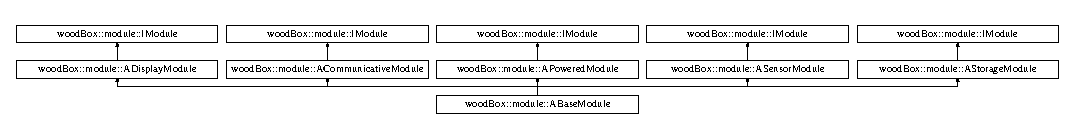
\includegraphics[height=3.000000cm]{classwood_box_1_1module_1_1_a_base_module}
\end{center}
\end{figure}
\subsection*{Public Member Functions}
\begin{DoxyCompactItemize}
\item 
\mbox{\Hypertarget{classwood_box_1_1module_1_1_a_base_module_a61e8f78a69b3ea735e70a13f6de8d662}\label{classwood_box_1_1module_1_1_a_base_module_a61e8f78a69b3ea735e70a13f6de8d662}} 
\mbox{\hyperlink{classwood_box_1_1module_1_1_a_base_module}{A\+Base\+Module}} \& {\bfseries operator=} (\mbox{\hyperlink{classwood_box_1_1module_1_1_a_base_module}{A\+Base\+Module}} \&)=delete
\item 
Stream $\ast$$\ast$ \mbox{\hyperlink{classwood_box_1_1module_1_1_a_base_module_ada9df5e73cb0aee0bada1de17de19a9c}{get\+Streams}} ()
\item 
void \mbox{\hyperlink{classwood_box_1_1module_1_1_a_base_module_a6e3b73bd36f668f5d621dee3070c131a}{set\+Streams}} (Stream $\ast$$\ast$)
\item 
\mbox{\hyperlink{classwood_box_1_1display_1_1_i_display}{display\+::\+I\+Display}} $\ast$ \mbox{\hyperlink{classwood_box_1_1module_1_1_a_base_module_afecd89a2ed85517a6d72ad2f03ea87c3}{get\+Display}} ()
\item 
void \mbox{\hyperlink{classwood_box_1_1module_1_1_a_base_module_a7e99b7d8d59953a8350e9859a475bc6a}{set\+Display}} (\mbox{\hyperlink{classwood_box_1_1display_1_1_i_display}{display\+::\+I\+Display}} $\ast$)
\item 
\mbox{\hyperlink{classwood_box_1_1power_1_1_i_power}{power\+::\+I\+Power}} $\ast$ \mbox{\hyperlink{classwood_box_1_1module_1_1_a_base_module_a1d67c7b9560b30774878e5b882c4bf0a}{get\+Power\+Source}} ()
\item 
void \mbox{\hyperlink{classwood_box_1_1module_1_1_a_base_module_a117ce9fbbcef048ccde38f0b6a11aa91}{set\+Power\+Source}} (\mbox{\hyperlink{classwood_box_1_1power_1_1_i_power}{power\+::\+I\+Power}} $\ast$)
\item 
\mbox{\hyperlink{classwood_box_1_1sensor_1_1_i_sensor}{sensor\+::\+I\+Sensor}} $\ast$ \mbox{\hyperlink{classwood_box_1_1module_1_1_a_base_module_acd7e95a20964a1f9ce2dbbbf629fe3dc}{get\+Sensor}} ()
\item 
void \mbox{\hyperlink{classwood_box_1_1module_1_1_a_base_module_ac3fd88feae532ca88b14642f76ef8def}{set\+Sensor}} (\mbox{\hyperlink{classwood_box_1_1sensor_1_1_i_sensor}{sensor\+::\+I\+Sensor}} $\ast$)
\item 
\mbox{\hyperlink{classwood_box_1_1storage_1_1_i_storage}{storage\+::\+I\+Storage}} $\ast$ \mbox{\hyperlink{classwood_box_1_1module_1_1_a_base_module_ad55a3509dc2bcb2fc5c8abc4a4db1cf1}{get\+Storage}} ()
\item 
void \mbox{\hyperlink{classwood_box_1_1module_1_1_a_base_module_af9e009af37d04062c2da7d977baded80}{set\+Storage}} (\mbox{\hyperlink{classwood_box_1_1storage_1_1_i_storage}{storage\+::\+I\+Storage}} $\ast$)
\end{DoxyCompactItemize}
\subsection*{Protected Member Functions}
\begin{DoxyCompactItemize}
\item 
\mbox{\Hypertarget{classwood_box_1_1module_1_1_a_base_module_a40edd799ba7342abfaf5cb06e60a4b04}\label{classwood_box_1_1module_1_1_a_base_module_a40edd799ba7342abfaf5cb06e60a4b04}} 
{\bfseries A\+Base\+Module} (\mbox{\hyperlink{classwood_box_1_1display_1_1_i_display}{display\+::\+I\+Display}} $\ast$=nullptr, Stream $\ast$$\ast$=nullptr, \mbox{\hyperlink{classwood_box_1_1power_1_1_i_power}{power\+::\+I\+Power}} $\ast$=nullptr, \mbox{\hyperlink{classwood_box_1_1sensor_1_1_i_sensor}{sensor\+::\+I\+Sensor}} $\ast$=nullptr, \mbox{\hyperlink{classwood_box_1_1storage_1_1_i_storage}{storage\+::\+I\+Storage}} $\ast$=nullptr)
\item 
\mbox{\Hypertarget{classwood_box_1_1module_1_1_a_base_module_a2ba8fdaace63960a0696b77bee60b64b}\label{classwood_box_1_1module_1_1_a_base_module_a2ba8fdaace63960a0696b77bee60b64b}} 
{\bfseries A\+Base\+Module} (\mbox{\hyperlink{classwood_box_1_1module_1_1_a_base_module}{A\+Base\+Module}} \&)=delete
\end{DoxyCompactItemize}
\subsection*{Protected Attributes}
\begin{DoxyCompactItemize}
\item 
\mbox{\Hypertarget{classwood_box_1_1module_1_1_a_base_module_a2550178f6fe0a97025e87da03a47d13f}\label{classwood_box_1_1module_1_1_a_base_module_a2550178f6fe0a97025e87da03a47d13f}} 
\mbox{\hyperlink{classwood_box_1_1display_1_1_i_display}{display\+::\+I\+Display}} $\ast$ {\bfseries \+\_\+display}
\item 
\mbox{\Hypertarget{classwood_box_1_1module_1_1_a_base_module_a851b365cdd36435e017297fcfdb8d5e8}\label{classwood_box_1_1module_1_1_a_base_module_a851b365cdd36435e017297fcfdb8d5e8}} 
Stream $\ast$$\ast$ {\bfseries \+\_\+streams}
\item 
\mbox{\Hypertarget{classwood_box_1_1module_1_1_a_base_module_a24c92fcd213167f9f917d6637a8df370}\label{classwood_box_1_1module_1_1_a_base_module_a24c92fcd213167f9f917d6637a8df370}} 
\mbox{\hyperlink{classwood_box_1_1power_1_1_i_power}{power\+::\+I\+Power}} $\ast$ {\bfseries \+\_\+power}
\item 
\mbox{\Hypertarget{classwood_box_1_1module_1_1_a_base_module_a9735d9e5169f0d26c2a9cf2fad3f12a5}\label{classwood_box_1_1module_1_1_a_base_module_a9735d9e5169f0d26c2a9cf2fad3f12a5}} 
\mbox{\hyperlink{classwood_box_1_1sensor_1_1_i_sensor}{sensor\+::\+I\+Sensor}} $\ast$ {\bfseries \+\_\+sensor}
\item 
\mbox{\Hypertarget{classwood_box_1_1module_1_1_a_base_module_aa187748e43497da9786e37c777948901}\label{classwood_box_1_1module_1_1_a_base_module_aa187748e43497da9786e37c777948901}} 
\mbox{\hyperlink{classwood_box_1_1storage_1_1_i_storage}{storage\+::\+I\+Storage}} $\ast$ {\bfseries \+\_\+storage}
\end{DoxyCompactItemize}


\subsection{Detailed Description}
Abstract base class for all Module classes, mainly handling low level logic and accessers to Module components 

\subsection{Member Function Documentation}
\mbox{\Hypertarget{classwood_box_1_1module_1_1_a_base_module_afecd89a2ed85517a6d72ad2f03ea87c3}\label{classwood_box_1_1module_1_1_a_base_module_afecd89a2ed85517a6d72ad2f03ea87c3}} 
\index{wood\+Box\+::module\+::\+A\+Base\+Module@{wood\+Box\+::module\+::\+A\+Base\+Module}!get\+Display@{get\+Display}}
\index{get\+Display@{get\+Display}!wood\+Box\+::module\+::\+A\+Base\+Module@{wood\+Box\+::module\+::\+A\+Base\+Module}}
\subsubsection{\texorpdfstring{get\+Display()}{getDisplay()}}
{\footnotesize\ttfamily \mbox{\hyperlink{classwood_box_1_1display_1_1_i_display}{display\+::\+I\+Display}} $\ast$ wood\+Box\+::module\+::\+A\+Base\+Module\+::get\+Display (\begin{DoxyParamCaption}{ }\end{DoxyParamCaption})}

Return a \mbox{\hyperlink{classwood_box_1_1display_1_1_i_display}{wood\+Box\+::display\+::\+I\+Display}} interface pointer on the display currently used by the module.

Warning\+: On some embedded targets there\textquotesingle{}s no C++ runtime (so no {\ttfamily dynamic\+\_\+cast} or {\ttfamily typeof}), the user will have to know and cast by himself this pointer to the correct type.

If there\textquotesingle{}s no display interface currently used by the module, this method returns {\ttfamily nullptr}. \mbox{\Hypertarget{classwood_box_1_1module_1_1_a_base_module_a1d67c7b9560b30774878e5b882c4bf0a}\label{classwood_box_1_1module_1_1_a_base_module_a1d67c7b9560b30774878e5b882c4bf0a}} 
\index{wood\+Box\+::module\+::\+A\+Base\+Module@{wood\+Box\+::module\+::\+A\+Base\+Module}!get\+Power\+Source@{get\+Power\+Source}}
\index{get\+Power\+Source@{get\+Power\+Source}!wood\+Box\+::module\+::\+A\+Base\+Module@{wood\+Box\+::module\+::\+A\+Base\+Module}}
\subsubsection{\texorpdfstring{get\+Power\+Source()}{getPowerSource()}}
{\footnotesize\ttfamily \mbox{\hyperlink{classwood_box_1_1power_1_1_i_power}{power\+::\+I\+Power}} $\ast$ wood\+Box\+::module\+::\+A\+Base\+Module\+::get\+Power\+Source (\begin{DoxyParamCaption}{ }\end{DoxyParamCaption})}

Return a \mbox{\hyperlink{classwood_box_1_1power_1_1_i_power}{wood\+Box\+::power\+::\+I\+Power}} interface pointer on the power supply currently used by the module.

Warning\+: On some embedded targets there\textquotesingle{}s no C++ runtime (so no {\ttfamily dynamic\+\_\+cast} or {\ttfamily typeof}), the user will have to know and cast by himself this pointer to the correct type.

If there\textquotesingle{}s no power interface currently used by the module, this method returns {\ttfamily nullptr}. \mbox{\Hypertarget{classwood_box_1_1module_1_1_a_base_module_acd7e95a20964a1f9ce2dbbbf629fe3dc}\label{classwood_box_1_1module_1_1_a_base_module_acd7e95a20964a1f9ce2dbbbf629fe3dc}} 
\index{wood\+Box\+::module\+::\+A\+Base\+Module@{wood\+Box\+::module\+::\+A\+Base\+Module}!get\+Sensor@{get\+Sensor}}
\index{get\+Sensor@{get\+Sensor}!wood\+Box\+::module\+::\+A\+Base\+Module@{wood\+Box\+::module\+::\+A\+Base\+Module}}
\subsubsection{\texorpdfstring{get\+Sensor()}{getSensor()}}
{\footnotesize\ttfamily \mbox{\hyperlink{classwood_box_1_1sensor_1_1_i_sensor}{sensor\+::\+I\+Sensor}} $\ast$ wood\+Box\+::module\+::\+A\+Base\+Module\+::get\+Sensor (\begin{DoxyParamCaption}{ }\end{DoxyParamCaption})}

Return a \mbox{\hyperlink{classwood_box_1_1sensor_1_1_i_sensor}{wood\+Box\+::sensor\+::\+I\+Sensor}} interface pointer on the sensor currently used by the module.

Warning\+: On some embedded targets there\textquotesingle{}s no C++ runtime (so no {\ttfamily dynamic\+\_\+cast} or {\ttfamily typeof}), the user will have to know and cast by himself this pointer to the correct type.

If there\textquotesingle{}s no sensor interface currently used by the module, this method returns {\ttfamily nullptr}. \mbox{\Hypertarget{classwood_box_1_1module_1_1_a_base_module_ad55a3509dc2bcb2fc5c8abc4a4db1cf1}\label{classwood_box_1_1module_1_1_a_base_module_ad55a3509dc2bcb2fc5c8abc4a4db1cf1}} 
\index{wood\+Box\+::module\+::\+A\+Base\+Module@{wood\+Box\+::module\+::\+A\+Base\+Module}!get\+Storage@{get\+Storage}}
\index{get\+Storage@{get\+Storage}!wood\+Box\+::module\+::\+A\+Base\+Module@{wood\+Box\+::module\+::\+A\+Base\+Module}}
\subsubsection{\texorpdfstring{get\+Storage()}{getStorage()}}
{\footnotesize\ttfamily \mbox{\hyperlink{classwood_box_1_1storage_1_1_i_storage}{storage\+::\+I\+Storage}} $\ast$ wood\+Box\+::module\+::\+A\+Base\+Module\+::get\+Storage (\begin{DoxyParamCaption}{ }\end{DoxyParamCaption})}

Return a \mbox{\hyperlink{classwood_box_1_1storage_1_1_i_storage}{wood\+Box\+::storage\+::\+I\+Storage}} interface pointer on the storage currently used by the module.

Warning\+: On some embedded targets there\textquotesingle{}s no C++ runtime (so no {\ttfamily dynamic\+\_\+cast} or {\ttfamily typeof}), the user will have to know and cast by himself this pointer to the correct type.

If there\textquotesingle{}s no storage interface currently used by the module, this method returns {\ttfamily nullptr}. \mbox{\Hypertarget{classwood_box_1_1module_1_1_a_base_module_ada9df5e73cb0aee0bada1de17de19a9c}\label{classwood_box_1_1module_1_1_a_base_module_ada9df5e73cb0aee0bada1de17de19a9c}} 
\index{wood\+Box\+::module\+::\+A\+Base\+Module@{wood\+Box\+::module\+::\+A\+Base\+Module}!get\+Streams@{get\+Streams}}
\index{get\+Streams@{get\+Streams}!wood\+Box\+::module\+::\+A\+Base\+Module@{wood\+Box\+::module\+::\+A\+Base\+Module}}
\subsubsection{\texorpdfstring{get\+Streams()}{getStreams()}}
{\footnotesize\ttfamily Stream $\ast$$\ast$ wood\+Box\+::module\+::\+A\+Base\+Module\+::get\+Streams (\begin{DoxyParamCaption}{ }\end{DoxyParamCaption})}

Return an array of pointers on {\ttfamily Stream} derived objects terminated by a {\ttfamily nullptr}.

For example, the array can be like this\+: {\ttfamily \{\&Serial, \&Serial1, \&\mbox{\hyperlink{classwood_box_1_1communication_1_1wifi_1_1_e_s_p8266_wi_fi_communicator}{wood\+Box\+::communication\+::wifi\+::\+E\+S\+P8266\+Wi\+Fi\+Communicator}}, nullptr\}}

If there\textquotesingle{}s no {\ttfamily Stream}s used by the module, this method returns {\ttfamily nullptr} \mbox{\Hypertarget{classwood_box_1_1module_1_1_a_base_module_a7e99b7d8d59953a8350e9859a475bc6a}\label{classwood_box_1_1module_1_1_a_base_module_a7e99b7d8d59953a8350e9859a475bc6a}} 
\index{wood\+Box\+::module\+::\+A\+Base\+Module@{wood\+Box\+::module\+::\+A\+Base\+Module}!set\+Display@{set\+Display}}
\index{set\+Display@{set\+Display}!wood\+Box\+::module\+::\+A\+Base\+Module@{wood\+Box\+::module\+::\+A\+Base\+Module}}
\subsubsection{\texorpdfstring{set\+Display()}{setDisplay()}}
{\footnotesize\ttfamily void wood\+Box\+::module\+::\+A\+Base\+Module\+::set\+Display (\begin{DoxyParamCaption}\item[{\mbox{\hyperlink{classwood_box_1_1display_1_1_i_display}{display\+::\+I\+Display}} $\ast$}]{display }\end{DoxyParamCaption})}

Set the pointer on the \mbox{\hyperlink{classwood_box_1_1display_1_1_i_display}{wood\+Box\+::display\+::\+I\+Display}} interface used by the module. \mbox{\Hypertarget{classwood_box_1_1module_1_1_a_base_module_a117ce9fbbcef048ccde38f0b6a11aa91}\label{classwood_box_1_1module_1_1_a_base_module_a117ce9fbbcef048ccde38f0b6a11aa91}} 
\index{wood\+Box\+::module\+::\+A\+Base\+Module@{wood\+Box\+::module\+::\+A\+Base\+Module}!set\+Power\+Source@{set\+Power\+Source}}
\index{set\+Power\+Source@{set\+Power\+Source}!wood\+Box\+::module\+::\+A\+Base\+Module@{wood\+Box\+::module\+::\+A\+Base\+Module}}
\subsubsection{\texorpdfstring{set\+Power\+Source()}{setPowerSource()}}
{\footnotesize\ttfamily void wood\+Box\+::module\+::\+A\+Base\+Module\+::set\+Power\+Source (\begin{DoxyParamCaption}\item[{\mbox{\hyperlink{classwood_box_1_1power_1_1_i_power}{power\+::\+I\+Power}} $\ast$}]{power }\end{DoxyParamCaption})}

Set the pointer on the \mbox{\hyperlink{classwood_box_1_1power_1_1_i_power}{wood\+Box\+::power\+::\+I\+Power}} interface used by the module. \mbox{\Hypertarget{classwood_box_1_1module_1_1_a_base_module_ac3fd88feae532ca88b14642f76ef8def}\label{classwood_box_1_1module_1_1_a_base_module_ac3fd88feae532ca88b14642f76ef8def}} 
\index{wood\+Box\+::module\+::\+A\+Base\+Module@{wood\+Box\+::module\+::\+A\+Base\+Module}!set\+Sensor@{set\+Sensor}}
\index{set\+Sensor@{set\+Sensor}!wood\+Box\+::module\+::\+A\+Base\+Module@{wood\+Box\+::module\+::\+A\+Base\+Module}}
\subsubsection{\texorpdfstring{set\+Sensor()}{setSensor()}}
{\footnotesize\ttfamily void wood\+Box\+::module\+::\+A\+Base\+Module\+::set\+Sensor (\begin{DoxyParamCaption}\item[{\mbox{\hyperlink{classwood_box_1_1sensor_1_1_i_sensor}{sensor\+::\+I\+Sensor}} $\ast$}]{sensor }\end{DoxyParamCaption})}

Set the pointer on the \mbox{\hyperlink{classwood_box_1_1sensor_1_1_i_sensor}{wood\+Box\+::sensor\+::\+I\+Sensor}} interface used by the module. \mbox{\Hypertarget{classwood_box_1_1module_1_1_a_base_module_af9e009af37d04062c2da7d977baded80}\label{classwood_box_1_1module_1_1_a_base_module_af9e009af37d04062c2da7d977baded80}} 
\index{wood\+Box\+::module\+::\+A\+Base\+Module@{wood\+Box\+::module\+::\+A\+Base\+Module}!set\+Storage@{set\+Storage}}
\index{set\+Storage@{set\+Storage}!wood\+Box\+::module\+::\+A\+Base\+Module@{wood\+Box\+::module\+::\+A\+Base\+Module}}
\subsubsection{\texorpdfstring{set\+Storage()}{setStorage()}}
{\footnotesize\ttfamily void wood\+Box\+::module\+::\+A\+Base\+Module\+::set\+Storage (\begin{DoxyParamCaption}\item[{\mbox{\hyperlink{classwood_box_1_1storage_1_1_i_storage}{storage\+::\+I\+Storage}} $\ast$}]{storage }\end{DoxyParamCaption})}

Set the pointer on the \mbox{\hyperlink{classwood_box_1_1storage_1_1_i_storage}{wood\+Box\+::storage\+::\+I\+Storage}} interface used by the module. \mbox{\Hypertarget{classwood_box_1_1module_1_1_a_base_module_a6e3b73bd36f668f5d621dee3070c131a}\label{classwood_box_1_1module_1_1_a_base_module_a6e3b73bd36f668f5d621dee3070c131a}} 
\index{wood\+Box\+::module\+::\+A\+Base\+Module@{wood\+Box\+::module\+::\+A\+Base\+Module}!set\+Streams@{set\+Streams}}
\index{set\+Streams@{set\+Streams}!wood\+Box\+::module\+::\+A\+Base\+Module@{wood\+Box\+::module\+::\+A\+Base\+Module}}
\subsubsection{\texorpdfstring{set\+Streams()}{setStreams()}}
{\footnotesize\ttfamily void wood\+Box\+::module\+::\+A\+Base\+Module\+::set\+Streams (\begin{DoxyParamCaption}\item[{Stream $\ast$$\ast$}]{streams }\end{DoxyParamCaption})}

Set the array of pointers on Stream derived objects used by module for communications.

For example\+: {\ttfamily Stream $\ast$my\+\_\+array\mbox{[}\mbox{]} = \{\&Serial, \&Serial1, \&\mbox{\hyperlink{classwood_box_1_1communication_1_1wifi_1_1_e_s_p8266_wi_fi_communicator}{wood\+Box\+::communication\+::wifi\+::\+E\+S\+P8266\+Wi\+Fi\+Communicator}}, nullptr\};} 

The documentation for this class was generated from the following files\+:\begin{DoxyCompactItemize}
\item 
A\+Base\+Module.\+hpp\item 
A\+Base\+Module.\+cpp\end{DoxyCompactItemize}

\hypertarget{classwood_box_1_1module_1_1_a_communicative_module}{}\section{wood\+Box\+:\+:module\+:\+:A\+Communicative\+Module Class Reference}
\label{classwood_box_1_1module_1_1_a_communicative_module}\index{wood\+Box\+::module\+::\+A\+Communicative\+Module@{wood\+Box\+::module\+::\+A\+Communicative\+Module}}
Inheritance diagram for wood\+Box\+:\+:module\+:\+:A\+Communicative\+Module\+:\begin{figure}[H]
\begin{center}
\leavevmode
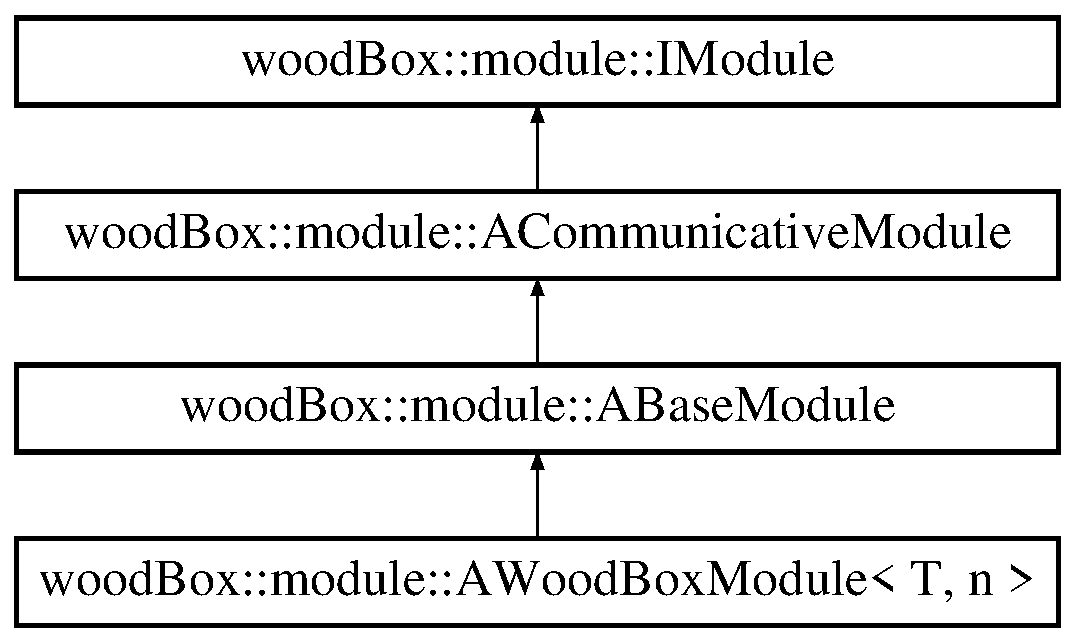
\includegraphics[height=3.000000cm]{classwood_box_1_1module_1_1_a_communicative_module}
\end{center}
\end{figure}
\subsection*{Public Member Functions}
\begin{DoxyCompactItemize}
\item 
\mbox{\Hypertarget{classwood_box_1_1module_1_1_a_communicative_module_afa4213c8224e42a60ac8412799064d50}\label{classwood_box_1_1module_1_1_a_communicative_module_afa4213c8224e42a60ac8412799064d50}} 
{\bfseries A\+Communicative\+Module} (\mbox{\hyperlink{classwood_box_1_1communication_1_1_i_communicator}{communication\+::\+I\+Communicator}} $\ast$)
\item 
\mbox{\Hypertarget{classwood_box_1_1module_1_1_a_communicative_module_af7d03d4e9ea7322b966af682f6106fd6}\label{classwood_box_1_1module_1_1_a_communicative_module_af7d03d4e9ea7322b966af682f6106fd6}} 
{\bfseries A\+Communicative\+Module} (\mbox{\hyperlink{classwood_box_1_1module_1_1_a_communicative_module}{A\+Communicative\+Module}} \&)
\item 
\mbox{\Hypertarget{classwood_box_1_1module_1_1_a_communicative_module_a2096b6a0f266d939000eb94b1b7275e3}\label{classwood_box_1_1module_1_1_a_communicative_module_a2096b6a0f266d939000eb94b1b7275e3}} 
virtual \mbox{\hyperlink{classwood_box_1_1module_1_1_a_communicative_module}{A\+Communicative\+Module}} \& {\bfseries operator=} (\mbox{\hyperlink{classwood_box_1_1module_1_1_a_communicative_module}{A\+Communicative\+Module}} \&)
\item 
\mbox{\Hypertarget{classwood_box_1_1module_1_1_a_communicative_module_afe8f1f438d36069c84818c7c2803266d}\label{classwood_box_1_1module_1_1_a_communicative_module_afe8f1f438d36069c84818c7c2803266d}} 
virtual void {\bfseries run} ()=0
\item 
\mbox{\Hypertarget{classwood_box_1_1module_1_1_a_communicative_module_aaedcc9c9798b58a7aed8cf615404ef31}\label{classwood_box_1_1module_1_1_a_communicative_module_aaedcc9c9798b58a7aed8cf615404ef31}} 
virtual void {\bfseries stop} ()=0
\item 
\mbox{\Hypertarget{classwood_box_1_1module_1_1_a_communicative_module_a30f015913ded87819d9e39266ad4f8ee}\label{classwood_box_1_1module_1_1_a_communicative_module_a30f015913ded87819d9e39266ad4f8ee}} 
virtual const \mbox{\hyperlink{classwood_box_1_1communication_1_1_i_communicator}{communication\+::\+I\+Communicator}} $\ast$ {\bfseries get\+Communicator} ()
\item 
\mbox{\Hypertarget{classwood_box_1_1module_1_1_a_communicative_module_af882e77775d892452247f0e6e7a008b7}\label{classwood_box_1_1module_1_1_a_communicative_module_af882e77775d892452247f0e6e7a008b7}} 
virtual void {\bfseries set\+Communicator} (\mbox{\hyperlink{classwood_box_1_1communication_1_1_i_communicator}{communication\+::\+I\+Communicator}} $\ast$)
\end{DoxyCompactItemize}
\subsection*{Protected Attributes}
\begin{DoxyCompactItemize}
\item 
\mbox{\Hypertarget{classwood_box_1_1module_1_1_a_communicative_module_a2eb402d7af8591b0935e79c63be06bf8}\label{classwood_box_1_1module_1_1_a_communicative_module_a2eb402d7af8591b0935e79c63be06bf8}} 
\mbox{\hyperlink{classwood_box_1_1communication_1_1_i_communicator}{communication\+::\+I\+Communicator}} $\ast$ {\bfseries \+\_\+stream}
\end{DoxyCompactItemize}


The documentation for this class was generated from the following files\+:\begin{DoxyCompactItemize}
\item 
A\+Communicative\+Module.\+hpp\item 
A\+Communicative\+Module.\+cpp\end{DoxyCompactItemize}

\hypertarget{classwood_box_1_1module_1_1_a_display_module}{}\section{wood\+Box\+:\+:module\+:\+:A\+Display\+Module Class Reference}
\label{classwood_box_1_1module_1_1_a_display_module}\index{wood\+Box\+::module\+::\+A\+Display\+Module@{wood\+Box\+::module\+::\+A\+Display\+Module}}
Inheritance diagram for wood\+Box\+:\+:module\+:\+:A\+Display\+Module\+:\begin{figure}[H]
\begin{center}
\leavevmode
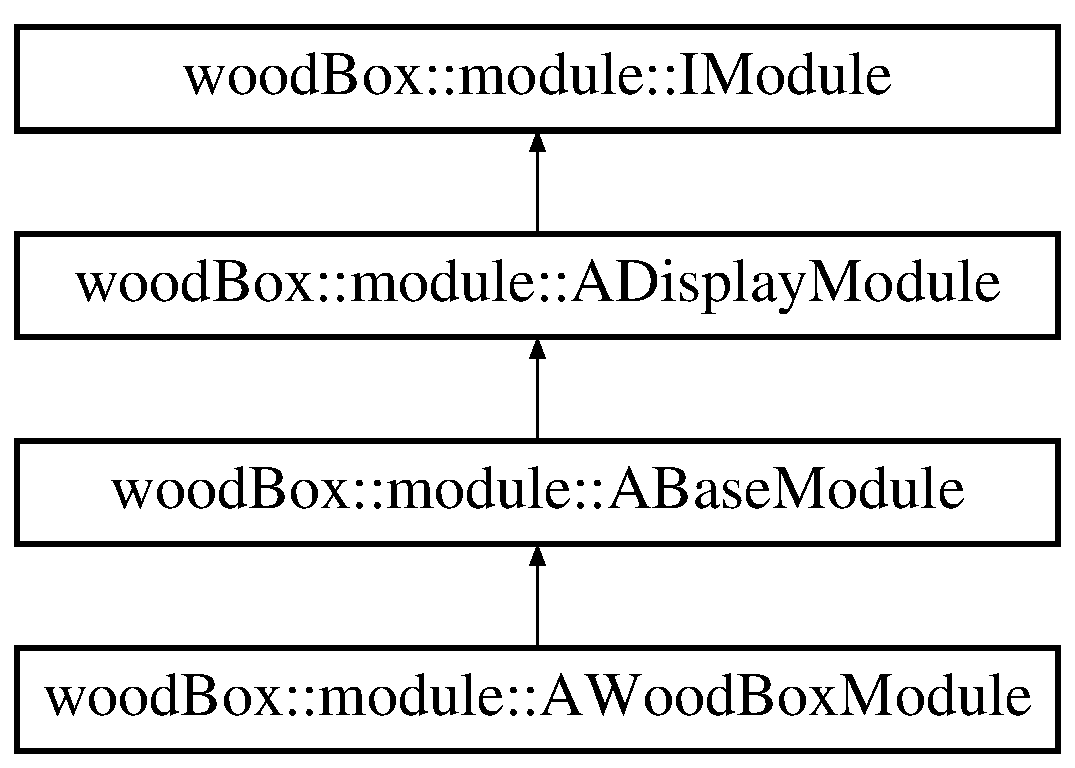
\includegraphics[height=3.000000cm]{classwood_box_1_1module_1_1_a_display_module}
\end{center}
\end{figure}
\subsection*{Public Member Functions}
\begin{DoxyCompactItemize}
\item 
\mbox{\Hypertarget{classwood_box_1_1module_1_1_a_display_module_ac53bf5dc049361072a8e2174aa27c8b3}\label{classwood_box_1_1module_1_1_a_display_module_ac53bf5dc049361072a8e2174aa27c8b3}} 
{\bfseries A\+Display\+Module} (\mbox{\hyperlink{classwood_box_1_1display_1_1_i_display}{display\+::\+I\+Display}} $\ast$)
\item 
\mbox{\Hypertarget{classwood_box_1_1module_1_1_a_display_module_af5124fa096f6ef17cae749a2dd8f5e0e}\label{classwood_box_1_1module_1_1_a_display_module_af5124fa096f6ef17cae749a2dd8f5e0e}} 
{\bfseries A\+Display\+Module} (\mbox{\hyperlink{classwood_box_1_1module_1_1_a_display_module}{A\+Display\+Module}} \&)
\item 
\mbox{\Hypertarget{classwood_box_1_1module_1_1_a_display_module_a41f26eb06fae670f21916724ac859302}\label{classwood_box_1_1module_1_1_a_display_module_a41f26eb06fae670f21916724ac859302}} 
virtual \mbox{\hyperlink{classwood_box_1_1module_1_1_a_display_module}{A\+Display\+Module}} \& {\bfseries operator=} (\mbox{\hyperlink{classwood_box_1_1module_1_1_a_display_module}{A\+Display\+Module}} \&)
\item 
\mbox{\Hypertarget{classwood_box_1_1module_1_1_a_display_module_a3b89ae22333f6fd4b9397ae24632b6d5}\label{classwood_box_1_1module_1_1_a_display_module_a3b89ae22333f6fd4b9397ae24632b6d5}} 
virtual void {\bfseries run} ()=0
\item 
\mbox{\Hypertarget{classwood_box_1_1module_1_1_a_display_module_a7cd0be127664613ee9c77a7d5b66c16e}\label{classwood_box_1_1module_1_1_a_display_module_a7cd0be127664613ee9c77a7d5b66c16e}} 
virtual void {\bfseries stop} ()=0
\item 
\mbox{\Hypertarget{classwood_box_1_1module_1_1_a_display_module_a048c746e97a75a4170a06bbc43d5ec15}\label{classwood_box_1_1module_1_1_a_display_module_a048c746e97a75a4170a06bbc43d5ec15}} 
virtual const \mbox{\hyperlink{classwood_box_1_1display_1_1_i_display}{display\+::\+I\+Display}} $\ast$ {\bfseries get\+Display} ()
\item 
\mbox{\Hypertarget{classwood_box_1_1module_1_1_a_display_module_a1fd524a64d867a9e4d23b35ea8c6e43f}\label{classwood_box_1_1module_1_1_a_display_module_a1fd524a64d867a9e4d23b35ea8c6e43f}} 
virtual void {\bfseries set\+Display} (\mbox{\hyperlink{classwood_box_1_1display_1_1_i_display}{display\+::\+I\+Display}} $\ast$)
\end{DoxyCompactItemize}
\subsection*{Protected Member Functions}
\begin{DoxyCompactItemize}
\item 
\mbox{\Hypertarget{classwood_box_1_1module_1_1_a_display_module_a4748a20ab717b105f60cd7cf6bef3983}\label{classwood_box_1_1module_1_1_a_display_module_a4748a20ab717b105f60cd7cf6bef3983}} 
virtual void {\bfseries on\+Update\+Display} ()=0
\end{DoxyCompactItemize}
\subsection*{Protected Attributes}
\begin{DoxyCompactItemize}
\item 
\mbox{\Hypertarget{classwood_box_1_1module_1_1_a_display_module_abd40ae3a519cd2b569631b6910ea342f}\label{classwood_box_1_1module_1_1_a_display_module_abd40ae3a519cd2b569631b6910ea342f}} 
\mbox{\hyperlink{classwood_box_1_1display_1_1_i_display}{display\+::\+I\+Display}} $\ast$ {\bfseries \+\_\+display}
\end{DoxyCompactItemize}


The documentation for this class was generated from the following files\+:\begin{DoxyCompactItemize}
\item 
A\+Display\+Module.\+hpp\item 
A\+Display\+Module.\+cpp\end{DoxyCompactItemize}

\hypertarget{classwood_box_1_1utility_1_1_a_iterable}{}\section{wood\+Box\+:\+:utility\+:\+:A\+Iterable$<$ T $>$ Class Template Reference}
\label{classwood_box_1_1utility_1_1_a_iterable}\index{wood\+Box\+::utility\+::\+A\+Iterable$<$ T $>$@{wood\+Box\+::utility\+::\+A\+Iterable$<$ T $>$}}
Inheritance diagram for wood\+Box\+:\+:utility\+:\+:A\+Iterable$<$ T $>$\+:\begin{figure}[H]
\begin{center}
\leavevmode
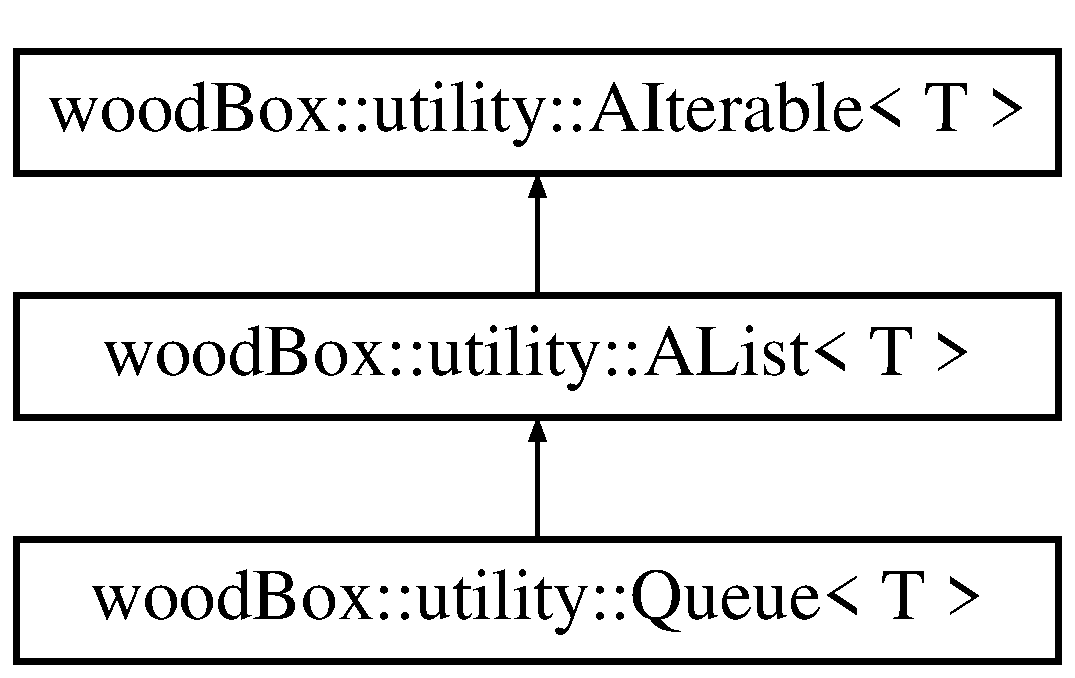
\includegraphics[height=3.000000cm]{classwood_box_1_1utility_1_1_a_iterable}
\end{center}
\end{figure}
\subsection*{Public Member Functions}
\begin{DoxyCompactItemize}
\item 
\mbox{\Hypertarget{classwood_box_1_1utility_1_1_a_iterable_aa8f6eb12adefa838343af8d8854ac7f6}\label{classwood_box_1_1utility_1_1_a_iterable_aa8f6eb12adefa838343af8d8854ac7f6}} 
{\bfseries A\+Iterable} (const \mbox{\hyperlink{classwood_box_1_1utility_1_1_a_iterable}{A\+Iterable}} \&other)=delete
\item 
\mbox{\Hypertarget{classwood_box_1_1utility_1_1_a_iterable_a9dfe1e1906628ef0892b50d12ba8696a}\label{classwood_box_1_1utility_1_1_a_iterable_a9dfe1e1906628ef0892b50d12ba8696a}} 
\mbox{\hyperlink{classwood_box_1_1utility_1_1_a_iterable}{A\+Iterable}} \& {\bfseries operator=} (const \mbox{\hyperlink{classwood_box_1_1utility_1_1_a_iterable}{A\+Iterable}} \&other)=delete
\item 
\mbox{\Hypertarget{classwood_box_1_1utility_1_1_a_iterable_a1ae4da148f184a6e95649c2e967389aa}\label{classwood_box_1_1utility_1_1_a_iterable_a1ae4da148f184a6e95649c2e967389aa}} 
T $\ast$ {\bfseries get} ()
\item 
\mbox{\Hypertarget{classwood_box_1_1utility_1_1_a_iterable_a675dfb37558f14704afeb50ab544f99f}\label{classwood_box_1_1utility_1_1_a_iterable_a675dfb37558f14704afeb50ab544f99f}} 
const T $\ast$ {\bfseries get} () const
\item 
\mbox{\Hypertarget{classwood_box_1_1utility_1_1_a_iterable_ae8978938416061fcfa2180ba2cd7f48c}\label{classwood_box_1_1utility_1_1_a_iterable_ae8978938416061fcfa2180ba2cd7f48c}} 
void {\bfseries set} (T $\ast$data)
\item 
\mbox{\Hypertarget{classwood_box_1_1utility_1_1_a_iterable_a3ddc252101ff34784456f0a3d712f4df}\label{classwood_box_1_1utility_1_1_a_iterable_a3ddc252101ff34784456f0a3d712f4df}} 
virtual \mbox{\hyperlink{classwood_box_1_1utility_1_1_a_iterable}{A\+Iterable}} $\ast$ {\bfseries next} ()=0
\item 
\mbox{\Hypertarget{classwood_box_1_1utility_1_1_a_iterable_a7d3afa98e4226f54e5b9671adec5d0ae}\label{classwood_box_1_1utility_1_1_a_iterable_a7d3afa98e4226f54e5b9671adec5d0ae}} 
virtual const \mbox{\hyperlink{classwood_box_1_1utility_1_1_a_iterable}{A\+Iterable}} $\ast$ {\bfseries next} () const =0
\end{DoxyCompactItemize}
\subsection*{Protected Member Functions}
\begin{DoxyCompactItemize}
\item 
\mbox{\Hypertarget{classwood_box_1_1utility_1_1_a_iterable_a9db8d4d69d94a3e0f230a6f9e8118c20}\label{classwood_box_1_1utility_1_1_a_iterable_a9db8d4d69d94a3e0f230a6f9e8118c20}} 
{\bfseries A\+Iterable} (T $\ast$data=nullptr)
\end{DoxyCompactItemize}


The documentation for this class was generated from the following file\+:\begin{DoxyCompactItemize}
\item 
A\+Iterable.\+hpp\end{DoxyCompactItemize}

\hypertarget{classwood_box_1_1utility_1_1_a_list}{}\section{wood\+Box\+:\+:utility\+:\+:A\+List$<$ T $>$ Class Template Reference}
\label{classwood_box_1_1utility_1_1_a_list}\index{wood\+Box\+::utility\+::\+A\+List$<$ T $>$@{wood\+Box\+::utility\+::\+A\+List$<$ T $>$}}


{\ttfamily \#include $<$A\+List.\+hpp$>$}

Inheritance diagram for wood\+Box\+:\+:utility\+:\+:A\+List$<$ T $>$\+:\begin{figure}[H]
\begin{center}
\leavevmode
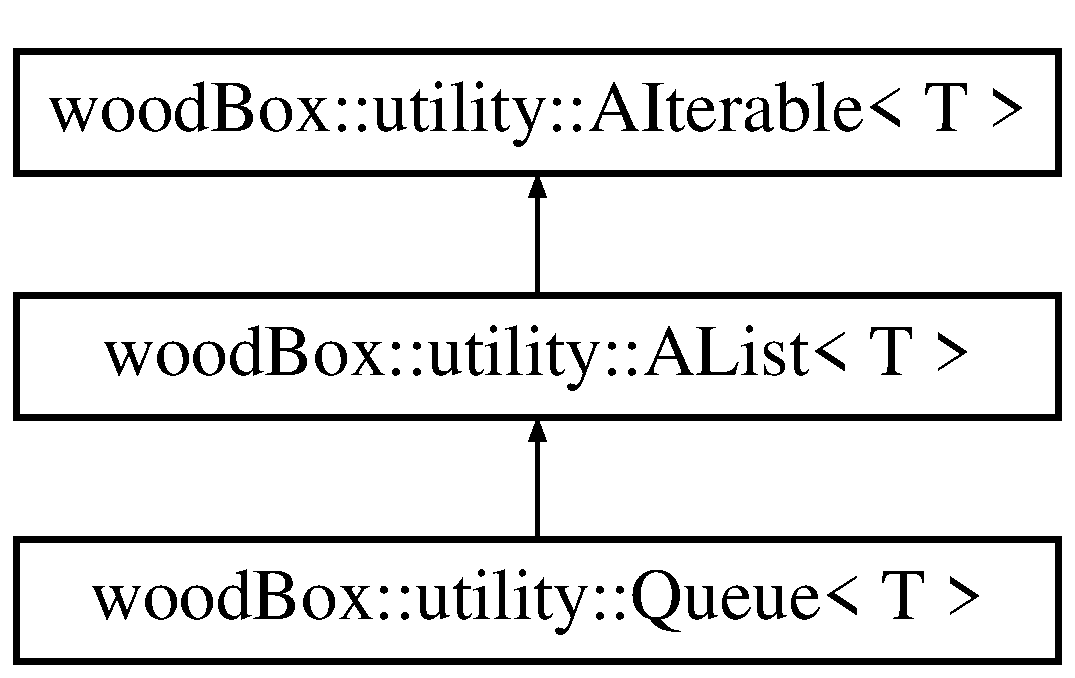
\includegraphics[height=3.000000cm]{classwood_box_1_1utility_1_1_a_list}
\end{center}
\end{figure}
\subsection*{Public Member Functions}
\begin{DoxyCompactItemize}
\item 
\mbox{\Hypertarget{classwood_box_1_1utility_1_1_a_list_a30c716d7e6462759801d1d3009ed5d13}\label{classwood_box_1_1utility_1_1_a_list_a30c716d7e6462759801d1d3009ed5d13}} 
\mbox{\hyperlink{classwood_box_1_1utility_1_1_a_list}{A\+List}} \& {\bfseries operator=} (const \mbox{\hyperlink{classwood_box_1_1utility_1_1_a_list}{A\+List}} \&other)=delete
\item 
\mbox{\Hypertarget{classwood_box_1_1utility_1_1_a_list_ae899fa889dc8909ee9cdffb2cdb0d2b4}\label{classwood_box_1_1utility_1_1_a_list_ae899fa889dc8909ee9cdffb2cdb0d2b4}} 
{\bfseries A\+List} (const \mbox{\hyperlink{classwood_box_1_1utility_1_1_a_list}{A\+List}} \&other)=delete
\item 
\mbox{\Hypertarget{classwood_box_1_1utility_1_1_a_list_ae3769cd3b298718c827026e8f17a2ece}\label{classwood_box_1_1utility_1_1_a_list_ae3769cd3b298718c827026e8f17a2ece}} 
virtual \mbox{\hyperlink{classwood_box_1_1utility_1_1_a_list}{A\+List}} $\ast$ {\bfseries next} ()
\item 
\mbox{\Hypertarget{classwood_box_1_1utility_1_1_a_list_a39e93ebf127847d1f8e7d99c8aa90c2e}\label{classwood_box_1_1utility_1_1_a_list_a39e93ebf127847d1f8e7d99c8aa90c2e}} 
virtual const \mbox{\hyperlink{classwood_box_1_1utility_1_1_a_list}{A\+List}} $\ast$ {\bfseries next} () const
\end{DoxyCompactItemize}
\subsection*{Protected Member Functions}
\begin{DoxyCompactItemize}
\item 
\mbox{\Hypertarget{classwood_box_1_1utility_1_1_a_list_a333eb2d9fa6833bba6675e2b5964ee4f}\label{classwood_box_1_1utility_1_1_a_list_a333eb2d9fa6833bba6675e2b5964ee4f}} 
{\bfseries A\+List} (\mbox{\hyperlink{classwood_box_1_1utility_1_1_a_list}{A\+List}} $\ast$next=nullptr, T $\ast$data=nullptr)
\item 
\mbox{\Hypertarget{classwood_box_1_1utility_1_1_a_list_adc24a832d3c7446cf1958eb9acfeb49b}\label{classwood_box_1_1utility_1_1_a_list_adc24a832d3c7446cf1958eb9acfeb49b}} 
void {\bfseries append} (\mbox{\hyperlink{classwood_box_1_1utility_1_1_a_list}{A\+List}} \&next)
\end{DoxyCompactItemize}
\subsection*{Protected Attributes}
\begin{DoxyCompactItemize}
\item 
\mbox{\Hypertarget{classwood_box_1_1utility_1_1_a_list_a843caa997ee9f3339b7e2b804acd11b7}\label{classwood_box_1_1utility_1_1_a_list_a843caa997ee9f3339b7e2b804acd11b7}} 
\mbox{\hyperlink{classwood_box_1_1utility_1_1_a_list}{A\+List}}$<$ T $>$ $\ast$ {\bfseries \+\_\+next}
\end{DoxyCompactItemize}


\subsection{Detailed Description}
\subsubsection*{template$<$typename T$>$\newline
class wood\+Box\+::utility\+::\+A\+List$<$ T $>$}

Class created for internal use of this library, but not used right now. Could be removed if considered useless. 

The documentation for this class was generated from the following file\+:\begin{DoxyCompactItemize}
\item 
A\+List.\+hpp\end{DoxyCompactItemize}

\hypertarget{classwood_box_1_1sensor_1_1_analog_sensor}{}\section{wood\+Box\+:\+:sensor\+:\+:Analog\+Sensor Class Reference}
\label{classwood_box_1_1sensor_1_1_analog_sensor}\index{wood\+Box\+::sensor\+::\+Analog\+Sensor@{wood\+Box\+::sensor\+::\+Analog\+Sensor}}
Inheritance diagram for wood\+Box\+:\+:sensor\+:\+:Analog\+Sensor\+:\begin{figure}[H]
\begin{center}
\leavevmode
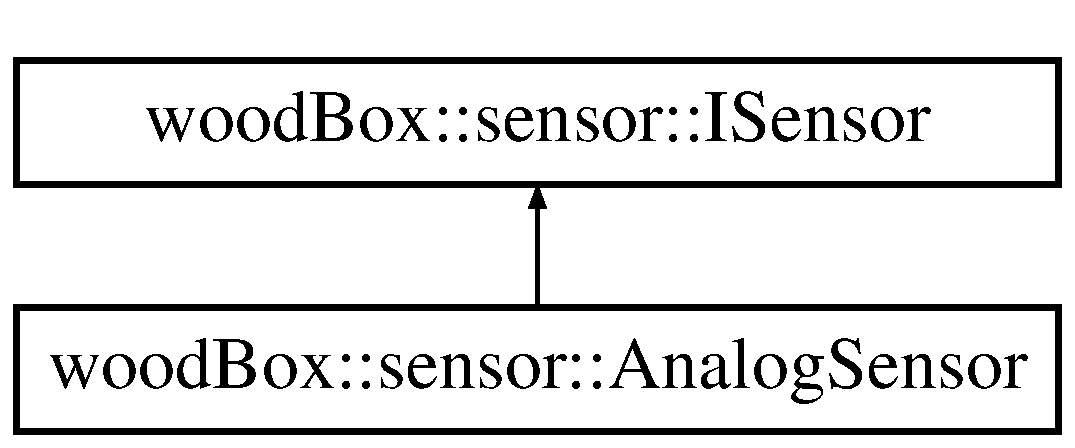
\includegraphics[height=2.000000cm]{classwood_box_1_1sensor_1_1_analog_sensor}
\end{center}
\end{figure}
\subsection*{Public Member Functions}
\begin{DoxyCompactItemize}
\item 
\mbox{\Hypertarget{classwood_box_1_1sensor_1_1_analog_sensor_a41d8ff91cf91d2bdbccffe8f1316421b}\label{classwood_box_1_1sensor_1_1_analog_sensor_a41d8ff91cf91d2bdbccffe8f1316421b}} 
{\bfseries Analog\+Sensor} (uint8\+\_\+t pin)
\item 
\mbox{\Hypertarget{classwood_box_1_1sensor_1_1_analog_sensor_a8ee0238d3fab4515b5286e67f1f92083}\label{classwood_box_1_1sensor_1_1_analog_sensor_a8ee0238d3fab4515b5286e67f1f92083}} 
{\bfseries Analog\+Sensor} (const \mbox{\hyperlink{classwood_box_1_1sensor_1_1_analog_sensor}{Analog\+Sensor}} \&)=delete
\item 
\mbox{\Hypertarget{classwood_box_1_1sensor_1_1_analog_sensor_a66111957aca931c1b1ea219749b03b3c}\label{classwood_box_1_1sensor_1_1_analog_sensor_a66111957aca931c1b1ea219749b03b3c}} 
\mbox{\hyperlink{classwood_box_1_1sensor_1_1_analog_sensor}{Analog\+Sensor}} \& {\bfseries operator=} (const \mbox{\hyperlink{classwood_box_1_1sensor_1_1_analog_sensor}{Analog\+Sensor}} \&)=delete
\item 
virtual uint8\+\_\+t $\ast$ \mbox{\hyperlink{classwood_box_1_1sensor_1_1_analog_sensor_ae78c25d8c01ba9acd03f90f278966189}{get\+Sample}} ()
\item 
virtual \mbox{\hyperlink{classwood_box_1_1sensor_1_1_i_sensor_aa377bda61ed0d4a1d7e1a7bffe459452}{I\+Sensor\+Scale}} \mbox{\hyperlink{classwood_box_1_1sensor_1_1_analog_sensor_a74ddcfe84f3f5b9d7010442f365c4eee}{get\+Estimate}} ()
\item 
\mbox{\Hypertarget{classwood_box_1_1sensor_1_1_analog_sensor_a5a7c67726db40be3edd48294910b117b}\label{classwood_box_1_1sensor_1_1_analog_sensor_a5a7c67726db40be3edd48294910b117b}} 
uint8\+\_\+t {\bfseries get\+Analogue\+Pin} ()
\end{DoxyCompactItemize}
\subsection*{Protected Attributes}
\begin{DoxyCompactItemize}
\item 
\mbox{\Hypertarget{classwood_box_1_1sensor_1_1_analog_sensor_a0377173a16668660f492c52694f96fab}\label{classwood_box_1_1sensor_1_1_analog_sensor_a0377173a16668660f492c52694f96fab}} 
uint8\+\_\+t {\bfseries \+\_\+analog\+\_\+pin}
\end{DoxyCompactItemize}
\subsection*{Additional Inherited Members}


\subsection{Member Function Documentation}
\mbox{\Hypertarget{classwood_box_1_1sensor_1_1_analog_sensor_a74ddcfe84f3f5b9d7010442f365c4eee}\label{classwood_box_1_1sensor_1_1_analog_sensor_a74ddcfe84f3f5b9d7010442f365c4eee}} 
\index{wood\+Box\+::sensor\+::\+Analog\+Sensor@{wood\+Box\+::sensor\+::\+Analog\+Sensor}!get\+Estimate@{get\+Estimate}}
\index{get\+Estimate@{get\+Estimate}!wood\+Box\+::sensor\+::\+Analog\+Sensor@{wood\+Box\+::sensor\+::\+Analog\+Sensor}}
\subsubsection{\texorpdfstring{get\+Estimate()}{getEstimate()}}
{\footnotesize\ttfamily \mbox{\hyperlink{classwood_box_1_1sensor_1_1_i_sensor_aa377bda61ed0d4a1d7e1a7bffe459452}{I\+Sensor\+::\+I\+Sensor\+Scale}} wood\+Box\+::sensor\+::\+Analog\+Sensor\+::get\+Estimate (\begin{DoxyParamCaption}{ }\end{DoxyParamCaption})\hspace{0.3cm}{\ttfamily [virtual]}}

Returns the estimation of safety from the current sensor value 

Implements \mbox{\hyperlink{classwood_box_1_1sensor_1_1_i_sensor_afb01c2473efc4a823bf5dada0048d2bc}{wood\+Box\+::sensor\+::\+I\+Sensor}}.

\mbox{\Hypertarget{classwood_box_1_1sensor_1_1_analog_sensor_ae78c25d8c01ba9acd03f90f278966189}\label{classwood_box_1_1sensor_1_1_analog_sensor_ae78c25d8c01ba9acd03f90f278966189}} 
\index{wood\+Box\+::sensor\+::\+Analog\+Sensor@{wood\+Box\+::sensor\+::\+Analog\+Sensor}!get\+Sample@{get\+Sample}}
\index{get\+Sample@{get\+Sample}!wood\+Box\+::sensor\+::\+Analog\+Sensor@{wood\+Box\+::sensor\+::\+Analog\+Sensor}}
\subsubsection{\texorpdfstring{get\+Sample()}{getSample()}}
{\footnotesize\ttfamily uint8\+\_\+t $\ast$ wood\+Box\+::sensor\+::\+Analog\+Sensor\+::get\+Sample (\begin{DoxyParamCaption}{ }\end{DoxyParamCaption})\hspace{0.3cm}{\ttfamily [virtual]}}

Returns a pointer on sensor sample raw memory, as an array of bytes 

Implements \mbox{\hyperlink{classwood_box_1_1sensor_1_1_i_sensor_a9de8041b991b76cc2f6fcc3b6a1bf363}{wood\+Box\+::sensor\+::\+I\+Sensor}}.



The documentation for this class was generated from the following files\+:\begin{DoxyCompactItemize}
\item 
Analog\+Sensor.\+hpp\item 
Analog\+Sensor.\+cpp\end{DoxyCompactItemize}

\hypertarget{classwood_box_1_1module_1_1_a_powered_module}{}\section{wood\+Box\+:\+:module\+:\+:A\+Powered\+Module Class Reference}
\label{classwood_box_1_1module_1_1_a_powered_module}\index{wood\+Box\+::module\+::\+A\+Powered\+Module@{wood\+Box\+::module\+::\+A\+Powered\+Module}}
Inheritance diagram for wood\+Box\+:\+:module\+:\+:A\+Powered\+Module\+:\begin{figure}[H]
\begin{center}
\leavevmode
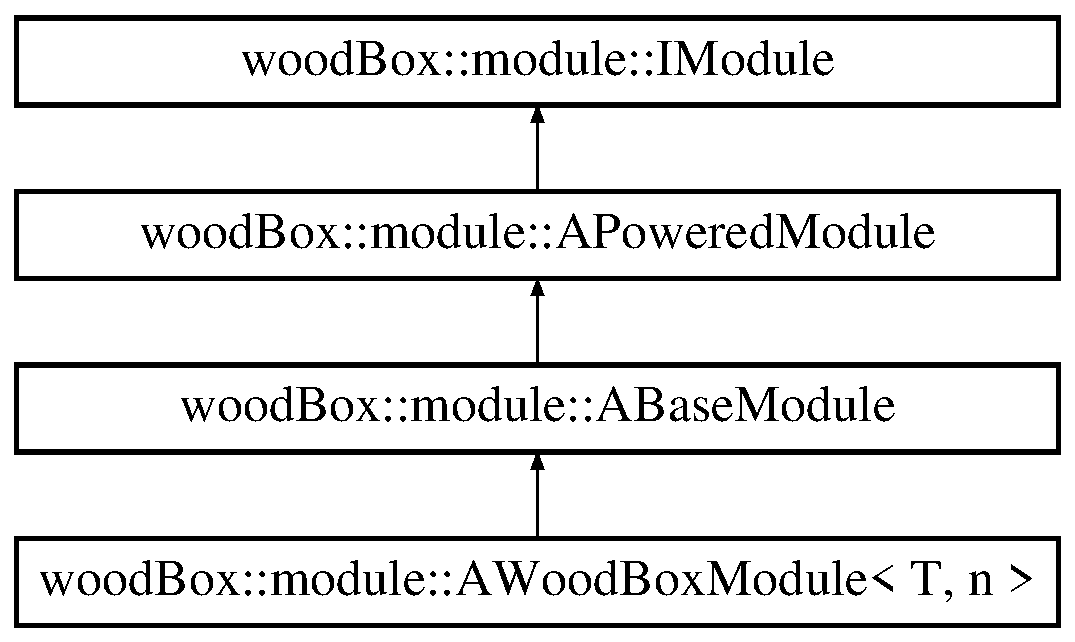
\includegraphics[height=4.000000cm]{classwood_box_1_1module_1_1_a_powered_module}
\end{center}
\end{figure}
\subsection*{Public Member Functions}
\begin{DoxyCompactItemize}
\item 
\mbox{\Hypertarget{classwood_box_1_1module_1_1_a_powered_module_ae46ff2edbf13a00b122c8d627833aca9}\label{classwood_box_1_1module_1_1_a_powered_module_ae46ff2edbf13a00b122c8d627833aca9}} 
{\bfseries A\+Powered\+Module} (\mbox{\hyperlink{classwood_box_1_1power_1_1_i_power}{power\+::\+I\+Power}} $\ast$)
\item 
\mbox{\Hypertarget{classwood_box_1_1module_1_1_a_powered_module_aa7b72c91f8fbc65e3bf199dea5d08147}\label{classwood_box_1_1module_1_1_a_powered_module_aa7b72c91f8fbc65e3bf199dea5d08147}} 
{\bfseries A\+Powered\+Module} (\mbox{\hyperlink{classwood_box_1_1module_1_1_a_powered_module}{A\+Powered\+Module}} \&)
\item 
\mbox{\Hypertarget{classwood_box_1_1module_1_1_a_powered_module_a656ef336760bd59f34821329cd4426f4}\label{classwood_box_1_1module_1_1_a_powered_module_a656ef336760bd59f34821329cd4426f4}} 
\mbox{\hyperlink{classwood_box_1_1module_1_1_a_powered_module}{A\+Powered\+Module}} \& {\bfseries operator=} (\mbox{\hyperlink{classwood_box_1_1module_1_1_a_powered_module}{A\+Powered\+Module}} \&)
\item 
\mbox{\Hypertarget{classwood_box_1_1module_1_1_a_powered_module_a1c381561d3bbf64e48dac5f1c56a75f9}\label{classwood_box_1_1module_1_1_a_powered_module_a1c381561d3bbf64e48dac5f1c56a75f9}} 
virtual void {\bfseries run} ()=0
\item 
\mbox{\Hypertarget{classwood_box_1_1module_1_1_a_powered_module_a452b60528326f5490ae6f0fd1ce2323d}\label{classwood_box_1_1module_1_1_a_powered_module_a452b60528326f5490ae6f0fd1ce2323d}} 
virtual void {\bfseries stop} ()=0
\item 
\mbox{\Hypertarget{classwood_box_1_1module_1_1_a_powered_module_a308ad31b0239b88e5a6338eb1442a0f2}\label{classwood_box_1_1module_1_1_a_powered_module_a308ad31b0239b88e5a6338eb1442a0f2}} 
virtual const \mbox{\hyperlink{classwood_box_1_1power_1_1_i_power}{power\+::\+I\+Power}} $\ast$ {\bfseries get\+Power\+Source} ()
\item 
\mbox{\Hypertarget{classwood_box_1_1module_1_1_a_powered_module_a750168a00d76a788095c739a64364ac4}\label{classwood_box_1_1module_1_1_a_powered_module_a750168a00d76a788095c739a64364ac4}} 
virtual void {\bfseries set\+Power\+Source} (\mbox{\hyperlink{classwood_box_1_1power_1_1_i_power}{power\+::\+I\+Power}} $\ast$)
\end{DoxyCompactItemize}
\subsection*{Protected Attributes}
\begin{DoxyCompactItemize}
\item 
\mbox{\Hypertarget{classwood_box_1_1module_1_1_a_powered_module_a897293dce32761f74ae234ae18634dba}\label{classwood_box_1_1module_1_1_a_powered_module_a897293dce32761f74ae234ae18634dba}} 
\mbox{\hyperlink{classwood_box_1_1power_1_1_i_power}{power\+::\+I\+Power}} $\ast$ {\bfseries \+\_\+power}
\end{DoxyCompactItemize}


The documentation for this class was generated from the following files\+:\begin{DoxyCompactItemize}
\item 
A\+Powered\+Module.\+hpp\item 
A\+Powered\+Module.\+cpp\end{DoxyCompactItemize}

\hypertarget{classwood_box_1_1module_1_1_a_sensor_module}{}\section{wood\+Box\+:\+:module\+:\+:A\+Sensor\+Module Class Reference}
\label{classwood_box_1_1module_1_1_a_sensor_module}\index{wood\+Box\+::module\+::\+A\+Sensor\+Module@{wood\+Box\+::module\+::\+A\+Sensor\+Module}}
Inheritance diagram for wood\+Box\+:\+:module\+:\+:A\+Sensor\+Module\+:\begin{figure}[H]
\begin{center}
\leavevmode
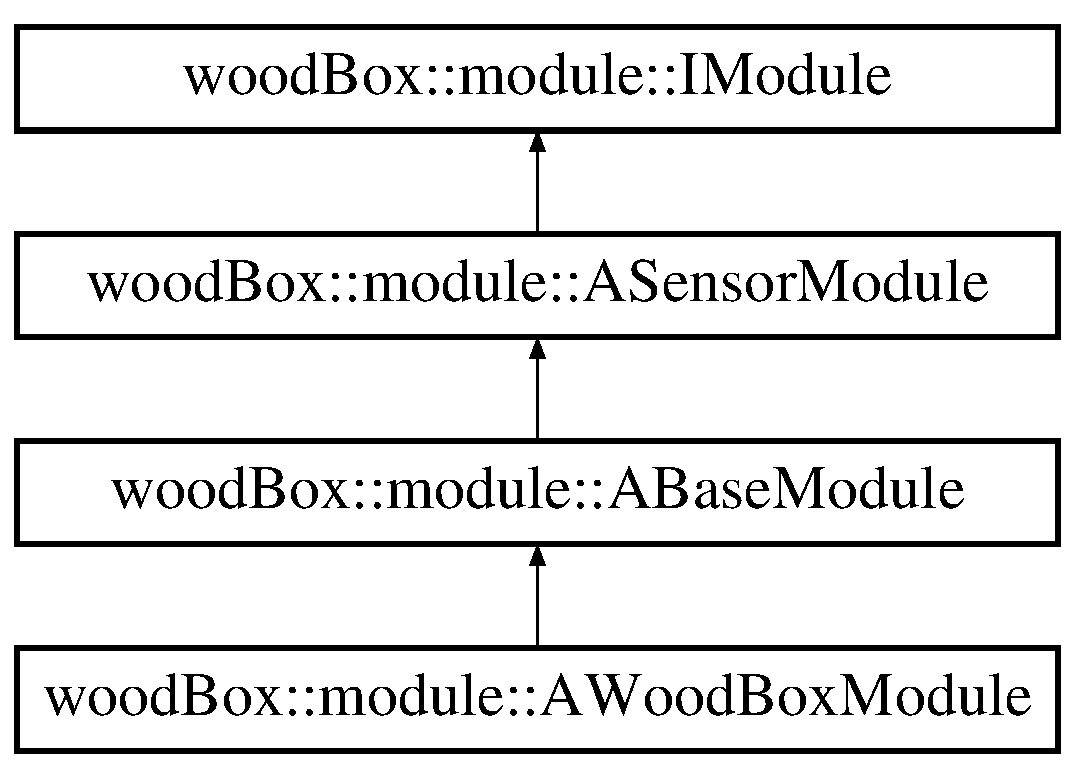
\includegraphics[height=4.000000cm]{classwood_box_1_1module_1_1_a_sensor_module}
\end{center}
\end{figure}
\subsection*{Public Member Functions}
\begin{DoxyCompactItemize}
\item 
\mbox{\Hypertarget{classwood_box_1_1module_1_1_a_sensor_module_a33708c35a41841cd3a39241b5ed739ef}\label{classwood_box_1_1module_1_1_a_sensor_module_a33708c35a41841cd3a39241b5ed739ef}} 
{\bfseries A\+Sensor\+Module} (\mbox{\hyperlink{classwood_box_1_1sensor_1_1_i_sensor}{sensor\+::\+I\+Sensor}} $\ast$sensor)
\item 
\mbox{\Hypertarget{classwood_box_1_1module_1_1_a_sensor_module_ab871ceaa91e971bb8c61dac5ffd9f019}\label{classwood_box_1_1module_1_1_a_sensor_module_ab871ceaa91e971bb8c61dac5ffd9f019}} 
{\bfseries A\+Sensor\+Module} (\mbox{\hyperlink{classwood_box_1_1module_1_1_a_sensor_module}{A\+Sensor\+Module}} \&)
\item 
\mbox{\Hypertarget{classwood_box_1_1module_1_1_a_sensor_module_a55c4c41e0e56ff8ec242d96b6588f1b6}\label{classwood_box_1_1module_1_1_a_sensor_module_a55c4c41e0e56ff8ec242d96b6588f1b6}} 
\mbox{\hyperlink{classwood_box_1_1module_1_1_a_sensor_module}{A\+Sensor\+Module}} \& {\bfseries operator=} (\mbox{\hyperlink{classwood_box_1_1module_1_1_a_sensor_module}{A\+Sensor\+Module}} \&)
\item 
\mbox{\Hypertarget{classwood_box_1_1module_1_1_a_sensor_module_a4fe5e01ec26cae47770229132f28bca9}\label{classwood_box_1_1module_1_1_a_sensor_module_a4fe5e01ec26cae47770229132f28bca9}} 
virtual void {\bfseries run} ()=0
\item 
\mbox{\Hypertarget{classwood_box_1_1module_1_1_a_sensor_module_ad40484d102c4a7b61d9f061613e78b20}\label{classwood_box_1_1module_1_1_a_sensor_module_ad40484d102c4a7b61d9f061613e78b20}} 
virtual void {\bfseries stop} ()=0
\item 
\mbox{\Hypertarget{classwood_box_1_1module_1_1_a_sensor_module_ab82cbdd06f385a40c323735b0ba5d28c}\label{classwood_box_1_1module_1_1_a_sensor_module_ab82cbdd06f385a40c323735b0ba5d28c}} 
virtual const \mbox{\hyperlink{classwood_box_1_1sensor_1_1_i_sensor}{sensor\+::\+I\+Sensor}} $\ast$ {\bfseries get\+Sensor} ()
\item 
\mbox{\Hypertarget{classwood_box_1_1module_1_1_a_sensor_module_ae5907b10855445076544ed1d3194dae8}\label{classwood_box_1_1module_1_1_a_sensor_module_ae5907b10855445076544ed1d3194dae8}} 
virtual void {\bfseries set\+Sensor} (\mbox{\hyperlink{classwood_box_1_1sensor_1_1_i_sensor}{sensor\+::\+I\+Sensor}} $\ast$)
\end{DoxyCompactItemize}
\subsection*{Protected Member Functions}
\begin{DoxyCompactItemize}
\item 
\mbox{\Hypertarget{classwood_box_1_1module_1_1_a_sensor_module_a8d32e6ff10ea54a75676786ca21bbefe}\label{classwood_box_1_1module_1_1_a_sensor_module_a8d32e6ff10ea54a75676786ca21bbefe}} 
virtual void {\bfseries on\+Sample\+Sensor} ()=0
\end{DoxyCompactItemize}
\subsection*{Protected Attributes}
\begin{DoxyCompactItemize}
\item 
\mbox{\Hypertarget{classwood_box_1_1module_1_1_a_sensor_module_adb99e18121febd3fe7edb084c3cad3f2}\label{classwood_box_1_1module_1_1_a_sensor_module_adb99e18121febd3fe7edb084c3cad3f2}} 
\mbox{\hyperlink{classwood_box_1_1sensor_1_1_i_sensor}{sensor\+::\+I\+Sensor}} $\ast$ {\bfseries \+\_\+sensor}
\end{DoxyCompactItemize}


The documentation for this class was generated from the following files\+:\begin{DoxyCompactItemize}
\item 
A\+Sensor\+Module.\+hpp\item 
A\+Sensor\+Module.\+cpp\end{DoxyCompactItemize}

\hypertarget{classwood_box_1_1module_1_1_a_storage_module}{}\section{wood\+Box\+:\+:module\+:\+:A\+Storage\+Module Class Reference}
\label{classwood_box_1_1module_1_1_a_storage_module}\index{wood\+Box\+::module\+::\+A\+Storage\+Module@{wood\+Box\+::module\+::\+A\+Storage\+Module}}
Inheritance diagram for wood\+Box\+:\+:module\+:\+:A\+Storage\+Module\+:\begin{figure}[H]
\begin{center}
\leavevmode
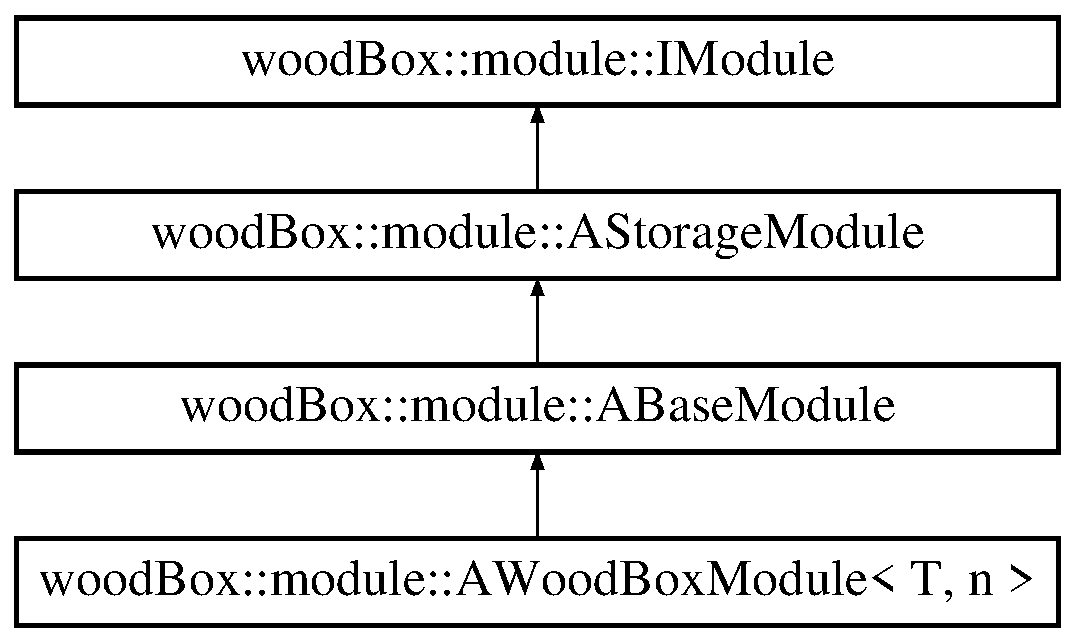
\includegraphics[height=3.000000cm]{classwood_box_1_1module_1_1_a_storage_module}
\end{center}
\end{figure}
\subsection*{Public Member Functions}
\begin{DoxyCompactItemize}
\item 
\mbox{\Hypertarget{classwood_box_1_1module_1_1_a_storage_module_a45a1e19acfb46e75c84fa2c8ce73a9fa}\label{classwood_box_1_1module_1_1_a_storage_module_a45a1e19acfb46e75c84fa2c8ce73a9fa}} 
{\bfseries A\+Storage\+Module} (\mbox{\hyperlink{classwood_box_1_1storage_1_1_i_storage}{storage\+::\+I\+Storage}} $\ast$)
\item 
\mbox{\Hypertarget{classwood_box_1_1module_1_1_a_storage_module_a741521f4ea295b17aaf39ad3dbb81b9a}\label{classwood_box_1_1module_1_1_a_storage_module_a741521f4ea295b17aaf39ad3dbb81b9a}} 
{\bfseries A\+Storage\+Module} (\mbox{\hyperlink{classwood_box_1_1module_1_1_a_storage_module}{A\+Storage\+Module}} \&)
\item 
\mbox{\Hypertarget{classwood_box_1_1module_1_1_a_storage_module_a88d6351c74fc81c3943c99d23abc2384}\label{classwood_box_1_1module_1_1_a_storage_module_a88d6351c74fc81c3943c99d23abc2384}} 
\mbox{\hyperlink{classwood_box_1_1module_1_1_a_storage_module}{A\+Storage\+Module}} \& {\bfseries operator=} (\mbox{\hyperlink{classwood_box_1_1module_1_1_a_storage_module}{A\+Storage\+Module}} \&)
\item 
\mbox{\Hypertarget{classwood_box_1_1module_1_1_a_storage_module_aac9b8d2704a4006dba34c20f3a7eb39f}\label{classwood_box_1_1module_1_1_a_storage_module_aac9b8d2704a4006dba34c20f3a7eb39f}} 
virtual void {\bfseries run} ()=0
\item 
\mbox{\Hypertarget{classwood_box_1_1module_1_1_a_storage_module_afc94649312f61e048495ec59ea0fa36c}\label{classwood_box_1_1module_1_1_a_storage_module_afc94649312f61e048495ec59ea0fa36c}} 
virtual void {\bfseries stop} ()=0
\item 
\mbox{\Hypertarget{classwood_box_1_1module_1_1_a_storage_module_a9d1453ac1813e3f2652360ed8367afd1}\label{classwood_box_1_1module_1_1_a_storage_module_a9d1453ac1813e3f2652360ed8367afd1}} 
virtual const \mbox{\hyperlink{classwood_box_1_1storage_1_1_i_storage}{storage\+::\+I\+Storage}} $\ast$ {\bfseries get\+Storage} ()
\item 
\mbox{\Hypertarget{classwood_box_1_1module_1_1_a_storage_module_a6f2eb352e676e12a228e8ec2d96bafc8}\label{classwood_box_1_1module_1_1_a_storage_module_a6f2eb352e676e12a228e8ec2d96bafc8}} 
virtual void {\bfseries set\+Storage} (\mbox{\hyperlink{classwood_box_1_1storage_1_1_i_storage}{storage\+::\+I\+Storage}} $\ast$)
\end{DoxyCompactItemize}
\subsection*{Protected Member Functions}
\begin{DoxyCompactItemize}
\item 
\mbox{\Hypertarget{classwood_box_1_1module_1_1_a_storage_module_ab105f7ff761ca9e4039fa1ee646cb8f6}\label{classwood_box_1_1module_1_1_a_storage_module_ab105f7ff761ca9e4039fa1ee646cb8f6}} 
virtual void {\bfseries on\+Backup\+On\+Storage} ()=0
\item 
\mbox{\Hypertarget{classwood_box_1_1module_1_1_a_storage_module_a6a2d3241b4424546eae140d217146ad8}\label{classwood_box_1_1module_1_1_a_storage_module_a6a2d3241b4424546eae140d217146ad8}} 
virtual void {\bfseries on\+Restore\+From\+Storage} ()=0
\end{DoxyCompactItemize}
\subsection*{Protected Attributes}
\begin{DoxyCompactItemize}
\item 
\mbox{\Hypertarget{classwood_box_1_1module_1_1_a_storage_module_ae9cc061f39337adb2b134e9ea378daa1}\label{classwood_box_1_1module_1_1_a_storage_module_ae9cc061f39337adb2b134e9ea378daa1}} 
\mbox{\hyperlink{classwood_box_1_1storage_1_1_i_storage}{storage\+::\+I\+Storage}} $\ast$ {\bfseries \+\_\+storage}
\end{DoxyCompactItemize}


The documentation for this class was generated from the following files\+:\begin{DoxyCompactItemize}
\item 
A\+Storage\+Module.\+hpp\item 
A\+Storage\+Module.\+cpp\end{DoxyCompactItemize}

\hypertarget{classwood_box_1_1communication_1_1wifi_1_1_a_wi_fi_communicator}{}\section{wood\+Box\+:\+:communication\+:\+:wifi\+:\+:A\+Wi\+Fi\+Communicator Class Reference}
\label{classwood_box_1_1communication_1_1wifi_1_1_a_wi_fi_communicator}\index{wood\+Box\+::communication\+::wifi\+::\+A\+Wi\+Fi\+Communicator@{wood\+Box\+::communication\+::wifi\+::\+A\+Wi\+Fi\+Communicator}}


{\ttfamily \#include $<$A\+Wi\+Fi\+Communicator.\+hpp$>$}

Inheritance diagram for wood\+Box\+:\+:communication\+:\+:wifi\+:\+:A\+Wi\+Fi\+Communicator\+:\begin{figure}[H]
\begin{center}
\leavevmode
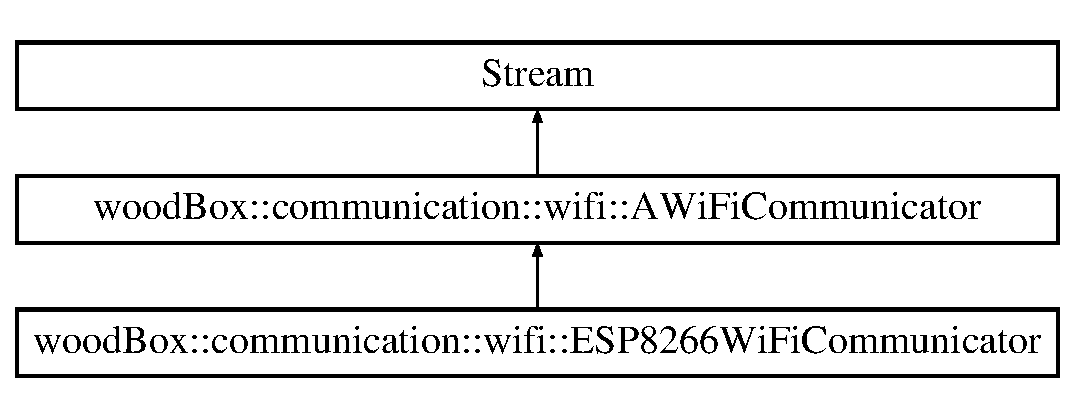
\includegraphics[height=3.000000cm]{classwood_box_1_1communication_1_1wifi_1_1_a_wi_fi_communicator}
\end{center}
\end{figure}
\subsection*{Public Member Functions}
\begin{DoxyCompactItemize}
\item 
\mbox{\hyperlink{classwood_box_1_1communication_1_1wifi_1_1_a_wi_fi_communicator_a9d1dc13ca9243170b04211bef2b86ed2}{A\+Wi\+Fi\+Communicator}} (const \mbox{\hyperlink{structwood_box_1_1communication_1_1wifi_1_1s__wifi__access__point}{Wi\+Fi\+\_\+ap}} $\ast$=nullptr, const \mbox{\hyperlink{structwood_box_1_1communication_1_1wifi_1_1s__wifi__client}{Wi\+Fi\+\_\+client}} $\ast$=nullptr, const wifi\+\_\+mode=S\+T\+A\+T\+I\+ON, Stream $\ast$=nullptr)
\item 
\mbox{\Hypertarget{classwood_box_1_1communication_1_1wifi_1_1_a_wi_fi_communicator_aef6faae3bf738776f0fb437a45c27883}\label{classwood_box_1_1communication_1_1wifi_1_1_a_wi_fi_communicator_aef6faae3bf738776f0fb437a45c27883}} 
{\bfseries A\+Wi\+Fi\+Communicator} (const \mbox{\hyperlink{classwood_box_1_1communication_1_1wifi_1_1_a_wi_fi_communicator}{A\+Wi\+Fi\+Communicator}} \&)=delete
\item 
\mbox{\Hypertarget{classwood_box_1_1communication_1_1wifi_1_1_a_wi_fi_communicator_a9f3c118a4268d09632f483aeb736a7c8}\label{classwood_box_1_1communication_1_1wifi_1_1_a_wi_fi_communicator_a9f3c118a4268d09632f483aeb736a7c8}} 
\mbox{\hyperlink{classwood_box_1_1communication_1_1wifi_1_1_a_wi_fi_communicator}{A\+Wi\+Fi\+Communicator}} \& {\bfseries operator=} (const \mbox{\hyperlink{classwood_box_1_1communication_1_1wifi_1_1_a_wi_fi_communicator}{A\+Wi\+Fi\+Communicator}} \&)=delete
\item 
virtual int \mbox{\hyperlink{classwood_box_1_1communication_1_1wifi_1_1_a_wi_fi_communicator_a541a26bf14cf77c13cc960963944ba1d}{available}} ()=0
\item 
virtual int \mbox{\hyperlink{classwood_box_1_1communication_1_1wifi_1_1_a_wi_fi_communicator_af4bc1adc96c124e769eb8c54d76476cf}{read}} ()=0
\item 
virtual int \mbox{\hyperlink{classwood_box_1_1communication_1_1wifi_1_1_a_wi_fi_communicator_ae0a1f2f1906f76a12dd5f9b7c10b1282}{peek}} ()=0
\item 
virtual size\+\_\+t \mbox{\hyperlink{classwood_box_1_1communication_1_1wifi_1_1_a_wi_fi_communicator_a7c40345fe59737b83bfee33ecb7be013}{write}} (uint8\+\_\+t)=0
\item 
virtual void \mbox{\hyperlink{classwood_box_1_1communication_1_1wifi_1_1_a_wi_fi_communicator_a1c74b8bc27a89604b4b7daa94c0168a6}{flush}} ()=0
\item 
virtual int \mbox{\hyperlink{classwood_box_1_1communication_1_1wifi_1_1_a_wi_fi_communicator_a7c4763c1594a4b934e5a39e90b271799}{connect}} ()=0
\item 
virtual int \mbox{\hyperlink{classwood_box_1_1communication_1_1wifi_1_1_a_wi_fi_communicator_ae0be1e1dd1e0508bdd2f348f0052f6e6}{disconnect}} ()=0
\item 
virtual int \mbox{\hyperlink{classwood_box_1_1communication_1_1wifi_1_1_a_wi_fi_communicator_ad8c31be391a58bfabe21c5ef99a94719}{connect\+To\+Host}} ()=0
\item 
virtual int \mbox{\hyperlink{classwood_box_1_1communication_1_1wifi_1_1_a_wi_fi_communicator_aeb87d8a22ad08c929c28191a4c725a5b}{disconnect\+From\+Host}} ()=0
\item 
virtual bool \mbox{\hyperlink{classwood_box_1_1communication_1_1wifi_1_1_a_wi_fi_communicator_afe42af0100dd483564995b8fc54b2e71}{is\+Connected}} ()=0
\item 
const \mbox{\hyperlink{structwood_box_1_1communication_1_1wifi_1_1s__wifi__access__point}{Wi\+Fi\+\_\+ap}} \& \mbox{\hyperlink{classwood_box_1_1communication_1_1wifi_1_1_a_wi_fi_communicator_abda6749593511b1acc44a999734b9bd6}{get\+Access\+Point}} () const
\item 
\mbox{\Hypertarget{classwood_box_1_1communication_1_1wifi_1_1_a_wi_fi_communicator_a9b0669461151786a0c70fbb1c1a07bc7}\label{classwood_box_1_1communication_1_1wifi_1_1_a_wi_fi_communicator_a9b0669461151786a0c70fbb1c1a07bc7}} 
const \mbox{\hyperlink{structwood_box_1_1communication_1_1wifi_1_1s__wifi__client}{Wi\+Fi\+\_\+client}} \& {\bfseries get\+Connection\+Addresses} () const
\item 
\mbox{\Hypertarget{classwood_box_1_1communication_1_1wifi_1_1_a_wi_fi_communicator_a6bd3193f145df44c577da0f0e7a8686a}\label{classwood_box_1_1communication_1_1wifi_1_1_a_wi_fi_communicator_a6bd3193f145df44c577da0f0e7a8686a}} 
const \mbox{\hyperlink{structwood_box_1_1communication_1_1ip_1_1s__host}{ip\+::tcp\+\_\+host}} \& {\bfseries get\+Host} () const
\item 
\mbox{\Hypertarget{classwood_box_1_1communication_1_1wifi_1_1_a_wi_fi_communicator_aa5b3e64e11585cb4ac16e7bd39fe565b}\label{classwood_box_1_1communication_1_1wifi_1_1_a_wi_fi_communicator_aa5b3e64e11585cb4ac16e7bd39fe565b}} 
wifi\+\_\+mode {\bfseries get\+Wi\+Fi\+Mode} () const
\item 
\mbox{\Hypertarget{classwood_box_1_1communication_1_1wifi_1_1_a_wi_fi_communicator_a6987322a622fab72d4a01de99da19491}\label{classwood_box_1_1communication_1_1wifi_1_1_a_wi_fi_communicator_a6987322a622fab72d4a01de99da19491}} 
void {\bfseries set\+Access\+Point} (const \mbox{\hyperlink{structwood_box_1_1communication_1_1wifi_1_1s__wifi__access__point}{Wi\+Fi\+\_\+ap}} \&)
\item 
\mbox{\Hypertarget{classwood_box_1_1communication_1_1wifi_1_1_a_wi_fi_communicator_ae0e96daf4cbeef3e646cc5af87eaa82d}\label{classwood_box_1_1communication_1_1wifi_1_1_a_wi_fi_communicator_ae0e96daf4cbeef3e646cc5af87eaa82d}} 
void {\bfseries set\+Connection\+Addresses} (const \mbox{\hyperlink{structwood_box_1_1communication_1_1wifi_1_1s__wifi__client}{Wi\+Fi\+\_\+client}} \&)
\item 
\mbox{\Hypertarget{classwood_box_1_1communication_1_1wifi_1_1_a_wi_fi_communicator_a1bbe3367296c647d6846b3c7d0313261}\label{classwood_box_1_1communication_1_1wifi_1_1_a_wi_fi_communicator_a1bbe3367296c647d6846b3c7d0313261}} 
void {\bfseries set\+Host} (const \mbox{\hyperlink{structwood_box_1_1communication_1_1ip_1_1s__host}{ip\+::tcp\+\_\+host}} \&)
\item 
\mbox{\Hypertarget{classwood_box_1_1communication_1_1wifi_1_1_a_wi_fi_communicator_a813fcffda64d86abfe0316a873f23f54}\label{classwood_box_1_1communication_1_1wifi_1_1_a_wi_fi_communicator_a813fcffda64d86abfe0316a873f23f54}} 
void {\bfseries set\+Wi\+Fi\+Mode} (wifi\+\_\+mode)
\item 
\mbox{\Hypertarget{classwood_box_1_1communication_1_1wifi_1_1_a_wi_fi_communicator_a526d2c9ece9000889fd40d9ab98acbdf}\label{classwood_box_1_1communication_1_1wifi_1_1_a_wi_fi_communicator_a526d2c9ece9000889fd40d9ab98acbdf}} 
void {\bfseries set\+Stream\+To\+Chipset} (Stream $\ast$)
\end{DoxyCompactItemize}
\subsection*{Protected Attributes}
\begin{DoxyCompactItemize}
\item 
\mbox{\Hypertarget{classwood_box_1_1communication_1_1wifi_1_1_a_wi_fi_communicator_ac07f090eb75730353a78f2d26f2095f1}\label{classwood_box_1_1communication_1_1wifi_1_1_a_wi_fi_communicator_ac07f090eb75730353a78f2d26f2095f1}} 
wifi\+\_\+mode {\bfseries \+\_\+mode}
\item 
\mbox{\Hypertarget{classwood_box_1_1communication_1_1wifi_1_1_a_wi_fi_communicator_a297970584d8120015f898afa1278eb46}\label{classwood_box_1_1communication_1_1wifi_1_1_a_wi_fi_communicator_a297970584d8120015f898afa1278eb46}} 
Stream $\ast$ {\bfseries \+\_\+stream}
\item 
\mbox{\Hypertarget{classwood_box_1_1communication_1_1wifi_1_1_a_wi_fi_communicator_a9d2cdaede0b5e5040867c3d428dd98f0}\label{classwood_box_1_1communication_1_1wifi_1_1_a_wi_fi_communicator_a9d2cdaede0b5e5040867c3d428dd98f0}} 
\mbox{\hyperlink{structwood_box_1_1communication_1_1wifi_1_1s__wifi__access__point}{Wi\+Fi\+\_\+ap}} {\bfseries \+\_\+ap}
\item 
\mbox{\Hypertarget{classwood_box_1_1communication_1_1wifi_1_1_a_wi_fi_communicator_afde4ef66d5296fbeeff2e1b333105bec}\label{classwood_box_1_1communication_1_1wifi_1_1_a_wi_fi_communicator_afde4ef66d5296fbeeff2e1b333105bec}} 
\mbox{\hyperlink{structwood_box_1_1communication_1_1wifi_1_1s__wifi__client}{Wi\+Fi\+\_\+client}} {\bfseries \+\_\+me}
\item 
\mbox{\Hypertarget{classwood_box_1_1communication_1_1wifi_1_1_a_wi_fi_communicator_ace744bc5d2c8f66dcd735029b129dea6}\label{classwood_box_1_1communication_1_1wifi_1_1_a_wi_fi_communicator_ace744bc5d2c8f66dcd735029b129dea6}} 
\mbox{\hyperlink{structwood_box_1_1communication_1_1ip_1_1s__host}{ip\+::tcp\+\_\+host}} {\bfseries \+\_\+host}
\end{DoxyCompactItemize}


\subsection{Detailed Description}
Abstract class derived from Stream, declaring some new Wi\+Fi common interface methods, and implementing some utility methods for these {\ttfamily Stream}s

Here\textquotesingle{}s a simple example of implementing a U\+A\+RT to Wi\+Fi chipset pre-\/configured to connect a Wi\+Fi network and transparently bridge the serial connection always connected to Serial Stream\+:


\begin{DoxyCode}
\textcolor{preprocessor}{#include <AWiFiCommunicator.hpp>}

\textcolor{keyword}{using} \mbox{\hyperlink{classwood_box_1_1communication_1_1wifi_1_1_a_wi_fi_communicator}{woodBox::communication::wifi::AWiFiCommunicator}};

\textcolor{keyword}{class }MyUARTBridge : \textcolor{keyword}{public} \mbox{\hyperlink{classwood_box_1_1communication_1_1wifi_1_1_a_wi_fi_communicator_a9d1dc13ca9243170b04211bef2b86ed2}{AWiFiCommunicator}} \{
  \textcolor{keyword}{public}:
    MyUARTBridge():\mbox{\hyperlink{classwood_box_1_1communication_1_1wifi_1_1_a_wi_fi_communicator_a9d1dc13ca9243170b04211bef2b86ed2}{AWiFiCommunicator}}() \{
      \_stream = &Serial;
    \}
    ~MyUARTBridge() \{\}

    \textcolor{keywordtype}{int} \mbox{\hyperlink{classwood_box_1_1communication_1_1wifi_1_1_a_wi_fi_communicator_a541a26bf14cf77c13cc960963944ba1d}{available}}() \{ \textcolor{keywordflow}{return} \_stream->available(); \}
    \textcolor{keywordtype}{int} \mbox{\hyperlink{classwood_box_1_1communication_1_1wifi_1_1_a_wi_fi_communicator_af4bc1adc96c124e769eb8c54d76476cf}{read}}() \{ \textcolor{keywordflow}{return} \_stream->return(); \}
    \textcolor{keywordtype}{int} \mbox{\hyperlink{classwood_box_1_1communication_1_1wifi_1_1_a_wi_fi_communicator_ae0a1f2f1906f76a12dd5f9b7c10b1282}{peek}}() \{ \textcolor{keywordflow}{return} \_stream->peek(); \}
    \textcolor{keywordtype}{size\_t} \mbox{\hyperlink{classwood_box_1_1communication_1_1wifi_1_1_a_wi_fi_communicator_a7c40345fe59737b83bfee33ecb7be013}{write}}(uint8\_t data) \{ \textcolor{keywordflow}{return} \_stream->write(data); \}
    \textcolor{keywordtype}{int} \mbox{\hyperlink{classwood_box_1_1communication_1_1wifi_1_1_a_wi_fi_communicator_a7c4763c1594a4b934e5a39e90b271799}{connect}}() \{ \textcolor{keywordflow}{return} 0; \}
    \textcolor{keywordtype}{int} \mbox{\hyperlink{classwood_box_1_1communication_1_1wifi_1_1_a_wi_fi_communicator_ae0be1e1dd1e0508bdd2f348f0052f6e6}{disconnect}}() \{ \textcolor{keywordflow}{return} 0; \}
    \textcolor{keywordtype}{int} \mbox{\hyperlink{classwood_box_1_1communication_1_1wifi_1_1_a_wi_fi_communicator_ad8c31be391a58bfabe21c5ef99a94719}{connectToHost}}() \{ \textcolor{keywordflow}{return} 0; \}
    \textcolor{keywordtype}{int} \mbox{\hyperlink{classwood_box_1_1communication_1_1wifi_1_1_a_wi_fi_communicator_aeb87d8a22ad08c929c28191a4c725a5b}{disconnectFromHost}}() \{ \textcolor{keywordflow}{return} 0; \}
    \textcolor{keywordtype}{bool} \mbox{\hyperlink{classwood_box_1_1communication_1_1wifi_1_1_a_wi_fi_communicator_afe42af0100dd483564995b8fc54b2e71}{isConnected}}() \{ \textcolor{keywordflow}{return} \textcolor{keyword}{true}; \}
\}
\end{DoxyCode}
 

\subsection{Constructor \& Destructor Documentation}
\mbox{\Hypertarget{classwood_box_1_1communication_1_1wifi_1_1_a_wi_fi_communicator_a9d1dc13ca9243170b04211bef2b86ed2}\label{classwood_box_1_1communication_1_1wifi_1_1_a_wi_fi_communicator_a9d1dc13ca9243170b04211bef2b86ed2}} 
\index{wood\+Box\+::communication\+::wifi\+::\+A\+Wi\+Fi\+Communicator@{wood\+Box\+::communication\+::wifi\+::\+A\+Wi\+Fi\+Communicator}!A\+Wi\+Fi\+Communicator@{A\+Wi\+Fi\+Communicator}}
\index{A\+Wi\+Fi\+Communicator@{A\+Wi\+Fi\+Communicator}!wood\+Box\+::communication\+::wifi\+::\+A\+Wi\+Fi\+Communicator@{wood\+Box\+::communication\+::wifi\+::\+A\+Wi\+Fi\+Communicator}}
\subsubsection{\texorpdfstring{A\+Wi\+Fi\+Communicator()}{AWiFiCommunicator()}}
{\footnotesize\ttfamily wood\+Box\+::communication\+::wifi\+::\+A\+Wi\+Fi\+Communicator\+::\+A\+Wi\+Fi\+Communicator (\begin{DoxyParamCaption}\item[{const \mbox{\hyperlink{structwood_box_1_1communication_1_1wifi_1_1s__wifi__access__point}{Wi\+Fi\+\_\+ap}} $\ast$}]{ap = {\ttfamily nullptr},  }\item[{const \mbox{\hyperlink{structwood_box_1_1communication_1_1wifi_1_1s__wifi__client}{Wi\+Fi\+\_\+client}} $\ast$}]{client = {\ttfamily nullptr},  }\item[{const wifi\+\_\+mode}]{mode = {\ttfamily STATION},  }\item[{Stream $\ast$}]{stream = {\ttfamily nullptr} }\end{DoxyParamCaption})}

Base constructor taking optional parameters to initialize instance attributes. 

\subsection{Member Function Documentation}
\mbox{\Hypertarget{classwood_box_1_1communication_1_1wifi_1_1_a_wi_fi_communicator_a541a26bf14cf77c13cc960963944ba1d}\label{classwood_box_1_1communication_1_1wifi_1_1_a_wi_fi_communicator_a541a26bf14cf77c13cc960963944ba1d}} 
\index{wood\+Box\+::communication\+::wifi\+::\+A\+Wi\+Fi\+Communicator@{wood\+Box\+::communication\+::wifi\+::\+A\+Wi\+Fi\+Communicator}!available@{available}}
\index{available@{available}!wood\+Box\+::communication\+::wifi\+::\+A\+Wi\+Fi\+Communicator@{wood\+Box\+::communication\+::wifi\+::\+A\+Wi\+Fi\+Communicator}}
\subsubsection{\texorpdfstring{available()}{available()}}
{\footnotesize\ttfamily virtual int wood\+Box\+::communication\+::wifi\+::\+A\+Wi\+Fi\+Communicator\+::available (\begin{DoxyParamCaption}{ }\end{DoxyParamCaption})\hspace{0.3cm}{\ttfamily [pure virtual]}}

Virtual method inherited from Stream interface. \href{https://www.arduino.cc/reference/en/language/functions/communication/stream/streamavailable/}{\tt See documentation on Arduino reference.} 

Implemented in \mbox{\hyperlink{classwood_box_1_1communication_1_1wifi_1_1_e_s_p8266_wi_fi_communicator_aa73f46aaaf5441b79dd4a15be293aeb4}{wood\+Box\+::communication\+::wifi\+::\+E\+S\+P8266\+Wi\+Fi\+Communicator}}.

\mbox{\Hypertarget{classwood_box_1_1communication_1_1wifi_1_1_a_wi_fi_communicator_a7c4763c1594a4b934e5a39e90b271799}\label{classwood_box_1_1communication_1_1wifi_1_1_a_wi_fi_communicator_a7c4763c1594a4b934e5a39e90b271799}} 
\index{wood\+Box\+::communication\+::wifi\+::\+A\+Wi\+Fi\+Communicator@{wood\+Box\+::communication\+::wifi\+::\+A\+Wi\+Fi\+Communicator}!connect@{connect}}
\index{connect@{connect}!wood\+Box\+::communication\+::wifi\+::\+A\+Wi\+Fi\+Communicator@{wood\+Box\+::communication\+::wifi\+::\+A\+Wi\+Fi\+Communicator}}
\subsubsection{\texorpdfstring{connect()}{connect()}}
{\footnotesize\ttfamily virtual int wood\+Box\+::communication\+::wifi\+::\+A\+Wi\+Fi\+Communicator\+::connect (\begin{DoxyParamCaption}{ }\end{DoxyParamCaption})\hspace{0.3cm}{\ttfamily [pure virtual]}}

Virtual method used to implement connection to Wi\+Fi network through the adapter.

A return value of 0 is expected to indicate the connection was successful, otherwise all other values are available for error codes.

Example\+:


\begin{DoxyCode}
\textcolor{preprocessor}{#include <string.h>}
\textcolor{preprocessor}{#include <woodBox.h>}

\textcolor{keyword}{using} \mbox{\hyperlink{structwood_box_1_1communication_1_1wifi_1_1s__wifi__access__point}{woodBox::communication::wifi::WiFi\_ap}}; \textcolor{comment}{// Use this to not have
       to write the full namespace names further}
\textcolor{keyword}{using} \mbox{\hyperlink{classwood_box_1_1communication_1_1wifi_1_1_a_wi_fi_communicator}{woodBox::communication::wifi::AWiFiCommunicator}};

\textcolor{keywordtype}{void} my\_function\_connecting\_wifi\_to\_network\_called\_foobar(\mbox{\hyperlink{classwood_box_1_1communication_1_1wifi_1_1_a_wi_fi_communicator_a9d1dc13ca9243170b04211bef2b86ed2}{AWiFiCommunicator}} &wifi) \{
  WiFi\_ap network; \textcolor{comment}{// Declare a WiFi\_ap structure}
  strcpy(network.ssid, \textcolor{stringliteral}{"foobar"}); \textcolor{comment}{// Copy "foobar" in the ssid field of the structure, as the SSID of a
       WiFi network is the name shown to humans}
  strcpy(network.password, \textcolor{stringliteral}{"12345678"}); \textcolor{comment}{// Copy "12345678" in the password field, to set the password used
       by the WiFi network}
  wifi.setAccessPoint(network); \textcolor{comment}{// Set the WiFi network parameters we created}
  \textcolor{keywordflow}{if} (!wifi.connect()) \{ \textcolor{comment}{// Connect to this network}
    Serial.println(\textcolor{stringliteral}{"Successfully connected to WiFi network"});
  \} \textcolor{keywordflow}{else} \{
    Serial.println(\textcolor{stringliteral}{"Connection to WiFi network failed"});
  \}
\}
\end{DoxyCode}
 

Implemented in \mbox{\hyperlink{classwood_box_1_1communication_1_1wifi_1_1_e_s_p8266_wi_fi_communicator_ab3e1f12a851dc3ed6eb487c39178cb6f}{wood\+Box\+::communication\+::wifi\+::\+E\+S\+P8266\+Wi\+Fi\+Communicator}}.

\mbox{\Hypertarget{classwood_box_1_1communication_1_1wifi_1_1_a_wi_fi_communicator_ad8c31be391a58bfabe21c5ef99a94719}\label{classwood_box_1_1communication_1_1wifi_1_1_a_wi_fi_communicator_ad8c31be391a58bfabe21c5ef99a94719}} 
\index{wood\+Box\+::communication\+::wifi\+::\+A\+Wi\+Fi\+Communicator@{wood\+Box\+::communication\+::wifi\+::\+A\+Wi\+Fi\+Communicator}!connect\+To\+Host@{connect\+To\+Host}}
\index{connect\+To\+Host@{connect\+To\+Host}!wood\+Box\+::communication\+::wifi\+::\+A\+Wi\+Fi\+Communicator@{wood\+Box\+::communication\+::wifi\+::\+A\+Wi\+Fi\+Communicator}}
\subsubsection{\texorpdfstring{connect\+To\+Host()}{connectToHost()}}
{\footnotesize\ttfamily virtual int wood\+Box\+::communication\+::wifi\+::\+A\+Wi\+Fi\+Communicator\+::connect\+To\+Host (\begin{DoxyParamCaption}{ }\end{DoxyParamCaption})\hspace{0.3cm}{\ttfamily [pure virtual]}}

Virtual method used to connect adapter to a socket on a host.

A return value of 0 is expected to indicate success, otherwise all other values are available for error codes.

Example\+:


\begin{DoxyCode}
\textcolor{preprocessor}{#include <woodBox.h>}

\textcolor{keyword}{using} \mbox{\hyperlink{structwood_box_1_1communication_1_1ip_1_1s__host}{woodBox::communication::ip::tcp\_host}}; \textcolor{comment}{// Use this to not have to
       write the full namespace names further}
\textcolor{keyword}{using} \mbox{\hyperlink{structwood_box_1_1communication_1_1wifi_1_1s__wifi__client}{woodBox::communication::wifi::WiFi\_client}};
\textcolor{keyword}{using} \mbox{\hyperlink{classwood_box_1_1communication_1_1wifi_1_1_a_wi_fi_communicator}{woodBox::communication::wifi::AWiFiCommunicator}};

\textcolor{keywordtype}{void} my\_function\_connecting\_to\_http\_port\_on\_router(\mbox{\hyperlink{classwood_box_1_1communication_1_1wifi_1_1_a_wi_fi_communicator_a9d1dc13ca9243170b04211bef2b86ed2}{AWiFiCommunicator}} &wifi) \{
  \textcolor{keyword}{const} WiFi\_client &my\_ip = wifi.getConnectionAddresses(); \textcolor{comment}{// Get our actual MAC and IP (IPv4 or IPv6)
       addresses}
  tcp\_host router = \{\{my\_ip.ipv4[0], my\_ip.ipv4[1], my\_ip.ipv4[2], 1\}, 80\}; \textcolor{comment}{// Use our current IPv4 address
       to deduce the one of the router, which often is the same as ours but ending with the value 1}
  wifi.setHost(router); \textcolor{comment}{// Set the new host to connect on, our structure tcp\_host is a couple IP + port}
  \textcolor{keywordflow}{if} (!wifi.connectToHost()) \{ \textcolor{comment}{// Connect to the socket on the host}
    Serial.println(\textcolor{stringliteral}{"Successfully connected to host"});
  \} \textcolor{keywordflow}{else} \{
    Serial.println(\textcolor{stringliteral}{"Failed to connect to host"});
  \}
\}
\end{DoxyCode}
 

Implemented in \mbox{\hyperlink{classwood_box_1_1communication_1_1wifi_1_1_e_s_p8266_wi_fi_communicator_a0875cf7209c48069d22270eaeb2cac0f}{wood\+Box\+::communication\+::wifi\+::\+E\+S\+P8266\+Wi\+Fi\+Communicator}}.

\mbox{\Hypertarget{classwood_box_1_1communication_1_1wifi_1_1_a_wi_fi_communicator_ae0be1e1dd1e0508bdd2f348f0052f6e6}\label{classwood_box_1_1communication_1_1wifi_1_1_a_wi_fi_communicator_ae0be1e1dd1e0508bdd2f348f0052f6e6}} 
\index{wood\+Box\+::communication\+::wifi\+::\+A\+Wi\+Fi\+Communicator@{wood\+Box\+::communication\+::wifi\+::\+A\+Wi\+Fi\+Communicator}!disconnect@{disconnect}}
\index{disconnect@{disconnect}!wood\+Box\+::communication\+::wifi\+::\+A\+Wi\+Fi\+Communicator@{wood\+Box\+::communication\+::wifi\+::\+A\+Wi\+Fi\+Communicator}}
\subsubsection{\texorpdfstring{disconnect()}{disconnect()}}
{\footnotesize\ttfamily virtual int wood\+Box\+::communication\+::wifi\+::\+A\+Wi\+Fi\+Communicator\+::disconnect (\begin{DoxyParamCaption}{ }\end{DoxyParamCaption})\hspace{0.3cm}{\ttfamily [pure virtual]}}

Virtual method used to implement disconnection of the current Wi\+Fi network through the adapter.

A return value of 0 is expected to indicate success, otherwise all other values are available for error codes.

Usage is as simple as this\+:


\begin{DoxyCode}
\textcolor{preprocessor}{#include <AWiFiCommunicator.hpp>}

\textcolor{keyword}{using} \mbox{\hyperlink{classwood_box_1_1communication_1_1wifi_1_1_a_wi_fi_communicator}{woodBox::communication::wifi::AWiFiCommunicator}};

\textcolor{keywordtype}{void} my\_function\_disconnecting\_wifi\_adapters(AWiFiCommuncator &wifi) \{
  \textcolor{keywordflow}{if} (!wifi.disconnect()) \{
    Serial.println(\textcolor{stringliteral}{"Successfully disconnected from WiFi network"});
  \} \textcolor{keywordflow}{else} \{
    Serial.println(\textcolor{stringliteral}{"Failed to disconnect from WiFi network"}); \textcolor{comment}{// Is that really possible? In case we're
       stuck, it's a problem where the "have you tried turning it off and on again?" rocks ;)}
\}
\end{DoxyCode}
 

Implemented in \mbox{\hyperlink{classwood_box_1_1communication_1_1wifi_1_1_e_s_p8266_wi_fi_communicator_af30a81a7f279c11241b3df0878289af0}{wood\+Box\+::communication\+::wifi\+::\+E\+S\+P8266\+Wi\+Fi\+Communicator}}.

\mbox{\Hypertarget{classwood_box_1_1communication_1_1wifi_1_1_a_wi_fi_communicator_aeb87d8a22ad08c929c28191a4c725a5b}\label{classwood_box_1_1communication_1_1wifi_1_1_a_wi_fi_communicator_aeb87d8a22ad08c929c28191a4c725a5b}} 
\index{wood\+Box\+::communication\+::wifi\+::\+A\+Wi\+Fi\+Communicator@{wood\+Box\+::communication\+::wifi\+::\+A\+Wi\+Fi\+Communicator}!disconnect\+From\+Host@{disconnect\+From\+Host}}
\index{disconnect\+From\+Host@{disconnect\+From\+Host}!wood\+Box\+::communication\+::wifi\+::\+A\+Wi\+Fi\+Communicator@{wood\+Box\+::communication\+::wifi\+::\+A\+Wi\+Fi\+Communicator}}
\subsubsection{\texorpdfstring{disconnect\+From\+Host()}{disconnectFromHost()}}
{\footnotesize\ttfamily virtual int wood\+Box\+::communication\+::wifi\+::\+A\+Wi\+Fi\+Communicator\+::disconnect\+From\+Host (\begin{DoxyParamCaption}{ }\end{DoxyParamCaption})\hspace{0.3cm}{\ttfamily [pure virtual]}}

Virtual method to disconnect from the current host, closing the socket.

A return value of 0 is expected to indicate success, otherwise all other values are available for error codes.

Example\+:


\begin{DoxyCode}
\textcolor{preprocessor}{#include <AWiFiCommunicator.hpp>}

\textcolor{keyword}{using} \mbox{\hyperlink{classwood_box_1_1communication_1_1wifi_1_1_a_wi_fi_communicator}{woodBox::communication::wifi::AWiFiCommunicator}};

\textcolor{keywordtype}{void} my\_function\_disconnecting\_an\_adapter\_from\_host(\mbox{\hyperlink{classwood_box_1_1communication_1_1wifi_1_1_a_wi_fi_communicator_a9d1dc13ca9243170b04211bef2b86ed2}{AWiFiCommunicator}} &wifi) \{
  \textcolor{keywordflow}{if} (!wifi.disconnectFromHost()) \{
    Serial.println(\textcolor{stringliteral}{"Successfully disconnected from host"});
  \} \textcolor{keywordflow}{else} \{
    Serial.println(\textcolor{stringliteral}{"Failed to disconnect from host"}); \textcolor{comment}{// If that happens, see the same scenario on
       disconnect method to have the solution ;)}
  \}
\}
\end{DoxyCode}
 

Implemented in \mbox{\hyperlink{classwood_box_1_1communication_1_1wifi_1_1_e_s_p8266_wi_fi_communicator_a5a407734df1ae47ac32575fa6346cfd4}{wood\+Box\+::communication\+::wifi\+::\+E\+S\+P8266\+Wi\+Fi\+Communicator}}.

\mbox{\Hypertarget{classwood_box_1_1communication_1_1wifi_1_1_a_wi_fi_communicator_a1c74b8bc27a89604b4b7daa94c0168a6}\label{classwood_box_1_1communication_1_1wifi_1_1_a_wi_fi_communicator_a1c74b8bc27a89604b4b7daa94c0168a6}} 
\index{wood\+Box\+::communication\+::wifi\+::\+A\+Wi\+Fi\+Communicator@{wood\+Box\+::communication\+::wifi\+::\+A\+Wi\+Fi\+Communicator}!flush@{flush}}
\index{flush@{flush}!wood\+Box\+::communication\+::wifi\+::\+A\+Wi\+Fi\+Communicator@{wood\+Box\+::communication\+::wifi\+::\+A\+Wi\+Fi\+Communicator}}
\subsubsection{\texorpdfstring{flush()}{flush()}}
{\footnotesize\ttfamily virtual void wood\+Box\+::communication\+::wifi\+::\+A\+Wi\+Fi\+Communicator\+::flush (\begin{DoxyParamCaption}{ }\end{DoxyParamCaption})\hspace{0.3cm}{\ttfamily [pure virtual]}}

Virtual method inherited from Stream interface. \href{https://www.arduino.cc/reference/en/language/functions/communication/stream/streamflush/}{\tt See documentation on Arduino reference.} 

Implemented in \mbox{\hyperlink{classwood_box_1_1communication_1_1wifi_1_1_e_s_p8266_wi_fi_communicator_a523aec958ef48fa917621a560d964f40}{wood\+Box\+::communication\+::wifi\+::\+E\+S\+P8266\+Wi\+Fi\+Communicator}}.

\mbox{\Hypertarget{classwood_box_1_1communication_1_1wifi_1_1_a_wi_fi_communicator_abda6749593511b1acc44a999734b9bd6}\label{classwood_box_1_1communication_1_1wifi_1_1_a_wi_fi_communicator_abda6749593511b1acc44a999734b9bd6}} 
\index{wood\+Box\+::communication\+::wifi\+::\+A\+Wi\+Fi\+Communicator@{wood\+Box\+::communication\+::wifi\+::\+A\+Wi\+Fi\+Communicator}!get\+Access\+Point@{get\+Access\+Point}}
\index{get\+Access\+Point@{get\+Access\+Point}!wood\+Box\+::communication\+::wifi\+::\+A\+Wi\+Fi\+Communicator@{wood\+Box\+::communication\+::wifi\+::\+A\+Wi\+Fi\+Communicator}}
\subsubsection{\texorpdfstring{get\+Access\+Point()}{getAccessPoint()}}
{\footnotesize\ttfamily const \mbox{\hyperlink{structwood_box_1_1communication_1_1wifi_1_1s__wifi__access__point}{Wi\+Fi\+\_\+ap}} \& wood\+Box\+::communication\+::wifi\+::\+A\+Wi\+Fi\+Communicator\+::get\+Access\+Point (\begin{DoxyParamCaption}{ }\end{DoxyParamCaption}) const}

Method returning a reference on the current configured access point into the instance of \mbox{\hyperlink{classwood_box_1_1communication_1_1wifi_1_1_a_wi_fi_communicator}{A\+Wi\+Fi\+Communicator}}.

See wood\+Box\+::communication\+::wifi\+::\+Wi\+Fi\+\_\+ap for more information on the content of this structure.

Example\+:


\begin{DoxyCode}
\textcolor{preprocessor}{#include <woodBox.h>}

\textcolor{keyword}{using} \mbox{\hyperlink{structwood_box_1_1communication_1_1wifi_1_1s__wifi__access__point}{woodBox::communication::wifi::WiFi\_ap}};
\textcolor{keyword}{using} \mbox{\hyperlink{classwood_box_1_1communication_1_1wifi_1_1_a_wi_fi_communicator}{woodBox::communication::wifi::AWiFiCommunicator}};

\textcolor{keywordtype}{void} my\_function\_printing\_current\_access\_point\_info(\mbox{\hyperlink{classwood_box_1_1communication_1_1wifi_1_1_a_wi_fi_communicator_a9d1dc13ca9243170b04211bef2b86ed2}{AWiFiCommunicator}} &wifi) \{
  \textcolor{keyword}{const} WiFi\_ap &access\_point = wifi.getAccessPoint;
  Serial.print(\textcolor{stringliteral}{"Network name: "});
  Serial.println(access\_point.ssid);
  Serial.print(\textcolor{stringliteral}{"Password: "});
  Serial.println(access\_point.password);
\}
\end{DoxyCode}
 \mbox{\Hypertarget{classwood_box_1_1communication_1_1wifi_1_1_a_wi_fi_communicator_afe42af0100dd483564995b8fc54b2e71}\label{classwood_box_1_1communication_1_1wifi_1_1_a_wi_fi_communicator_afe42af0100dd483564995b8fc54b2e71}} 
\index{wood\+Box\+::communication\+::wifi\+::\+A\+Wi\+Fi\+Communicator@{wood\+Box\+::communication\+::wifi\+::\+A\+Wi\+Fi\+Communicator}!is\+Connected@{is\+Connected}}
\index{is\+Connected@{is\+Connected}!wood\+Box\+::communication\+::wifi\+::\+A\+Wi\+Fi\+Communicator@{wood\+Box\+::communication\+::wifi\+::\+A\+Wi\+Fi\+Communicator}}
\subsubsection{\texorpdfstring{is\+Connected()}{isConnected()}}
{\footnotesize\ttfamily virtual bool wood\+Box\+::communication\+::wifi\+::\+A\+Wi\+Fi\+Communicator\+::is\+Connected (\begin{DoxyParamCaption}{ }\end{DoxyParamCaption})\hspace{0.3cm}{\ttfamily [pure virtual]}}

Virtual method to know if the adapter is connected to a Wi\+Fi network.

Return true if the adapter is connected, otherwise return false;

Example\+:


\begin{DoxyCode}
\textcolor{preprocessor}{#include <AWiFiCommunicator.hpp>}

\textcolor{keyword}{using} \mbox{\hyperlink{classwood_box_1_1communication_1_1wifi_1_1_a_wi_fi_communicator}{woodBox::communication::wifi::AWiFiCommunicator}};

\textcolor{keywordtype}{void} my\_function\_printing\_if\_adapter\_is\_connected\_to\_network\_or\_not(
      \mbox{\hyperlink{classwood_box_1_1communication_1_1wifi_1_1_a_wi_fi_communicator_a9d1dc13ca9243170b04211bef2b86ed2}{AWiFiCommunicator}} &wifi) \{
  Serial.println((wifi.isConnected) ? \textcolor{stringliteral}{"Adapter is connected to WiFi network"} : \textcolor{stringliteral}{"Adapter isn't connected to
       WiFi network"});
\}
\end{DoxyCode}
 

Implemented in \mbox{\hyperlink{classwood_box_1_1communication_1_1wifi_1_1_e_s_p8266_wi_fi_communicator_a66b7f8adaae85dbf94062b1cd472d98a}{wood\+Box\+::communication\+::wifi\+::\+E\+S\+P8266\+Wi\+Fi\+Communicator}}.

\mbox{\Hypertarget{classwood_box_1_1communication_1_1wifi_1_1_a_wi_fi_communicator_ae0a1f2f1906f76a12dd5f9b7c10b1282}\label{classwood_box_1_1communication_1_1wifi_1_1_a_wi_fi_communicator_ae0a1f2f1906f76a12dd5f9b7c10b1282}} 
\index{wood\+Box\+::communication\+::wifi\+::\+A\+Wi\+Fi\+Communicator@{wood\+Box\+::communication\+::wifi\+::\+A\+Wi\+Fi\+Communicator}!peek@{peek}}
\index{peek@{peek}!wood\+Box\+::communication\+::wifi\+::\+A\+Wi\+Fi\+Communicator@{wood\+Box\+::communication\+::wifi\+::\+A\+Wi\+Fi\+Communicator}}
\subsubsection{\texorpdfstring{peek()}{peek()}}
{\footnotesize\ttfamily virtual int wood\+Box\+::communication\+::wifi\+::\+A\+Wi\+Fi\+Communicator\+::peek (\begin{DoxyParamCaption}{ }\end{DoxyParamCaption})\hspace{0.3cm}{\ttfamily [pure virtual]}}

Virtual method inherited from Stream interface. \href{https://www.arduino.cc/reference/en/language/functions/communication/stream/streampeek/}{\tt See documentation on Arduino reference.} 

Implemented in \mbox{\hyperlink{classwood_box_1_1communication_1_1wifi_1_1_e_s_p8266_wi_fi_communicator_accc6832fa7351cb977b9e3a805dc8107}{wood\+Box\+::communication\+::wifi\+::\+E\+S\+P8266\+Wi\+Fi\+Communicator}}.

\mbox{\Hypertarget{classwood_box_1_1communication_1_1wifi_1_1_a_wi_fi_communicator_af4bc1adc96c124e769eb8c54d76476cf}\label{classwood_box_1_1communication_1_1wifi_1_1_a_wi_fi_communicator_af4bc1adc96c124e769eb8c54d76476cf}} 
\index{wood\+Box\+::communication\+::wifi\+::\+A\+Wi\+Fi\+Communicator@{wood\+Box\+::communication\+::wifi\+::\+A\+Wi\+Fi\+Communicator}!read@{read}}
\index{read@{read}!wood\+Box\+::communication\+::wifi\+::\+A\+Wi\+Fi\+Communicator@{wood\+Box\+::communication\+::wifi\+::\+A\+Wi\+Fi\+Communicator}}
\subsubsection{\texorpdfstring{read()}{read()}}
{\footnotesize\ttfamily virtual int wood\+Box\+::communication\+::wifi\+::\+A\+Wi\+Fi\+Communicator\+::read (\begin{DoxyParamCaption}{ }\end{DoxyParamCaption})\hspace{0.3cm}{\ttfamily [pure virtual]}}

Virtual method inherited from Stream interface. \href{https://www.arduino.cc/reference/en/language/functions/communication/stream/streamread/}{\tt See documentation on Arduino reference.} 

Implemented in \mbox{\hyperlink{classwood_box_1_1communication_1_1wifi_1_1_e_s_p8266_wi_fi_communicator_a3bd1c8f72256e92c6dbdab9272fd3543}{wood\+Box\+::communication\+::wifi\+::\+E\+S\+P8266\+Wi\+Fi\+Communicator}}.

\mbox{\Hypertarget{classwood_box_1_1communication_1_1wifi_1_1_a_wi_fi_communicator_a7c40345fe59737b83bfee33ecb7be013}\label{classwood_box_1_1communication_1_1wifi_1_1_a_wi_fi_communicator_a7c40345fe59737b83bfee33ecb7be013}} 
\index{wood\+Box\+::communication\+::wifi\+::\+A\+Wi\+Fi\+Communicator@{wood\+Box\+::communication\+::wifi\+::\+A\+Wi\+Fi\+Communicator}!write@{write}}
\index{write@{write}!wood\+Box\+::communication\+::wifi\+::\+A\+Wi\+Fi\+Communicator@{wood\+Box\+::communication\+::wifi\+::\+A\+Wi\+Fi\+Communicator}}
\subsubsection{\texorpdfstring{write()}{write()}}
{\footnotesize\ttfamily virtual size\+\_\+t wood\+Box\+::communication\+::wifi\+::\+A\+Wi\+Fi\+Communicator\+::write (\begin{DoxyParamCaption}\item[{uint8\+\_\+t}]{ }\end{DoxyParamCaption})\hspace{0.3cm}{\ttfamily [pure virtual]}}

Virtual method inherited from Stream interface. \href{https://www.arduino.cc/en/Serial/Write}{\tt See documentation on Arduino reference.} 

Implemented in \mbox{\hyperlink{classwood_box_1_1communication_1_1wifi_1_1_e_s_p8266_wi_fi_communicator_a6bb904e5302da7ec3fefc6e9a896f5f8}{wood\+Box\+::communication\+::wifi\+::\+E\+S\+P8266\+Wi\+Fi\+Communicator}}.



The documentation for this class was generated from the following files\+:\begin{DoxyCompactItemize}
\item 
A\+Wi\+Fi\+Communicator.\+hpp\item 
A\+Wi\+Fi\+Communicator.\+cpp\end{DoxyCompactItemize}

\hypertarget{classwood_box_1_1module_1_1_a_wood_box_module}{}\section{wood\+Box\+:\+:module\+:\+:A\+Wood\+Box\+Module Class Reference}
\label{classwood_box_1_1module_1_1_a_wood_box_module}\index{wood\+Box\+::module\+::\+A\+Wood\+Box\+Module@{wood\+Box\+::module\+::\+A\+Wood\+Box\+Module}}
Inheritance diagram for wood\+Box\+:\+:module\+:\+:A\+Wood\+Box\+Module\+:\begin{figure}[H]
\begin{center}
\leavevmode
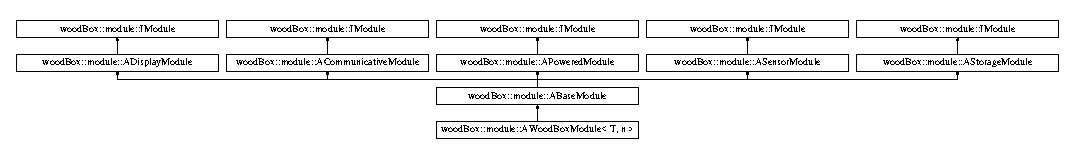
\includegraphics[height=1.729730cm]{classwood_box_1_1module_1_1_a_wood_box_module}
\end{center}
\end{figure}
\subsection*{Public Types}
\begin{DoxyCompactItemize}
\item 
\mbox{\Hypertarget{classwood_box_1_1module_1_1_a_wood_box_module_a9700d669ca2a36d350526c6b77dd2e1b}\label{classwood_box_1_1module_1_1_a_wood_box_module_a9700d669ca2a36d350526c6b77dd2e1b}} 
enum {\bfseries module\+Type} \{ \newline
{\bfseries A\+I\+R\+\_\+\+Q\+U\+A\+L\+I\+TY}, 
{\bfseries T\+E\+M\+P\+E\+R\+A\+T\+U\+RE}, 
{\bfseries H\+U\+M\+I\+D\+I\+TY}, 
{\bfseries L\+U\+M\+I\+N\+O\+S\+I\+TY}, 
\newline
{\bfseries N\+O\+I\+SE}, 
{\bfseries C\+A\+R\+B\+ON}, 
{\bfseries C\+A\+R\+B\+O\+N\+\_\+\+M\+O\+N\+O\+X\+Y\+DE}, 
{\bfseries E\+L\+E\+C\+T\+R\+O\+M\+A\+G\+N\+E\+T\+IC}, 
\newline
{\bfseries R\+A\+D\+I\+O\+A\+C\+T\+I\+V\+I\+TY}
 \}
\end{DoxyCompactItemize}
\subsection*{Public Member Functions}
\begin{DoxyCompactItemize}
\item 
\mbox{\Hypertarget{classwood_box_1_1module_1_1_a_wood_box_module_add6d18367bec65a3917f863b654c4319}\label{classwood_box_1_1module_1_1_a_wood_box_module_add6d18367bec65a3917f863b654c4319}} 
{\bfseries A\+Wood\+Box\+Module} (const \mbox{\hyperlink{classwood_box_1_1module_1_1_a_wood_box_module}{A\+Wood\+Box\+Module}} \&)=delete
\item 
\mbox{\Hypertarget{classwood_box_1_1module_1_1_a_wood_box_module_ae9f462f6e239ee6ea02cb0ece7c8e7b2}\label{classwood_box_1_1module_1_1_a_wood_box_module_ae9f462f6e239ee6ea02cb0ece7c8e7b2}} 
\mbox{\hyperlink{classwood_box_1_1module_1_1_a_wood_box_module}{A\+Wood\+Box\+Module}} \& {\bfseries operator=} (const \mbox{\hyperlink{classwood_box_1_1module_1_1_a_wood_box_module}{A\+Wood\+Box\+Module}} \&)=delete
\end{DoxyCompactItemize}
\subsection*{Public Attributes}
\begin{DoxyCompactItemize}
\item 
\mbox{\Hypertarget{classwood_box_1_1module_1_1_a_wood_box_module_af606a06208d58a95c65643d29e7d46e8}\label{classwood_box_1_1module_1_1_a_wood_box_module_af606a06208d58a95c65643d29e7d46e8}} 
char {\bfseries module\+Vendor} \mbox{[}33\mbox{]}
\item 
\mbox{\Hypertarget{classwood_box_1_1module_1_1_a_wood_box_module_a9786d6aaec0d2d1ce2f27b9f73f30c20}\label{classwood_box_1_1module_1_1_a_wood_box_module_a9786d6aaec0d2d1ce2f27b9f73f30c20}} 
char {\bfseries module\+Serial} \mbox{[}33\mbox{]}
\item 
\mbox{\Hypertarget{classwood_box_1_1module_1_1_a_wood_box_module_a6af0bda7216b8d2c5e0bf77c29c44613}\label{classwood_box_1_1module_1_1_a_wood_box_module_a6af0bda7216b8d2c5e0bf77c29c44613}} 
uint16\+\_\+t {\bfseries measure}
\item 
\mbox{\Hypertarget{classwood_box_1_1module_1_1_a_wood_box_module_a84edcbe776911c90e8dacc02d475c0d0}\label{classwood_box_1_1module_1_1_a_wood_box_module_a84edcbe776911c90e8dacc02d475c0d0}} 
uint32\+\_\+t {\bfseries timestamp}
\end{DoxyCompactItemize}
\subsection*{Additional Inherited Members}


The documentation for this class was generated from the following file\+:\begin{DoxyCompactItemize}
\item 
A\+Wood\+Box\+Module.\+hpp\end{DoxyCompactItemize}

\hypertarget{classwood_box_1_1utility_1_1_buffer}{}\section{wood\+Box\+:\+:utility\+:\+:Buffer$<$ T, size $>$ Class Template Reference}
\label{classwood_box_1_1utility_1_1_buffer}\index{wood\+Box\+::utility\+::\+Buffer$<$ T, size $>$@{wood\+Box\+::utility\+::\+Buffer$<$ T, size $>$}}


{\ttfamily \#include $<$Buffer.\+hpp$>$}

\subsection*{Public Member Functions}
\begin{DoxyCompactItemize}
\item 
\mbox{\Hypertarget{classwood_box_1_1utility_1_1_buffer_aebdfb364cf6e64092a1553231adb7a85}\label{classwood_box_1_1utility_1_1_buffer_aebdfb364cf6e64092a1553231adb7a85}} 
{\bfseries Buffer} (const \mbox{\hyperlink{classwood_box_1_1utility_1_1_buffer}{Buffer}} \&other)
\item 
\mbox{\Hypertarget{classwood_box_1_1utility_1_1_buffer_a051d336a9ee59bc40b7723ec3a54521e}\label{classwood_box_1_1utility_1_1_buffer_a051d336a9ee59bc40b7723ec3a54521e}} 
\mbox{\hyperlink{classwood_box_1_1utility_1_1_buffer}{Buffer}} \& {\bfseries operator=} (const \mbox{\hyperlink{classwood_box_1_1utility_1_1_buffer}{Buffer}} \&other)
\item 
void \mbox{\hyperlink{classwood_box_1_1utility_1_1_buffer_a2d7857dc93d7e229941ca36a018587e9}{write}} (T data)
\item 
T \mbox{\hyperlink{classwood_box_1_1utility_1_1_buffer_a8832f6e544e23f738ee50216d805572d}{read}} ()
\item 
int \mbox{\hyperlink{classwood_box_1_1utility_1_1_buffer_a2bcef18ccdd923a401608a257e4283ca}{available}} ()
\item 
T \mbox{\hyperlink{classwood_box_1_1utility_1_1_buffer_a9aa51ab0987fdbcfb72fccc1c806ba50}{peek}} ()
\item 
void \mbox{\hyperlink{classwood_box_1_1utility_1_1_buffer_a747e6bb3cd527dcf1651aa6758233666}{flush}} ()
\end{DoxyCompactItemize}


\subsection{Detailed Description}
\subsubsection*{template$<$typename T, size\+\_\+t size$>$\newline
class wood\+Box\+::utility\+::\+Buffer$<$ T, size $>$}

Templated buffer, taking as template parameters the type of hold data and their numbers.

Example of use\+:


\begin{DoxyCode}
\textcolor{preprocessor}{#include <Buffer.hpp>}
\textcolor{preprocessor}{#include <String.h>}

\textcolor{keyword}{using} \mbox{\hyperlink{classwood_box_1_1utility_1_1_buffer}{woodBox::utility::Buffer}};

String my\_string1(\textcolor{stringliteral}{"Hello, World!"});
String my\_string2(\textcolor{stringliteral}{"foobar"});
String my\_string3(\textcolor{stringliteral}{"Philipe ! Je sais ou tu te caches !"}); \textcolor{comment}{// Sorry for non-french readers :)}

\textcolor{keywordtype}{void} my\_function\_using\_a\_buffer() \{
  Buffer<const String &, 2> my\_buffer; \textcolor{comment}{// Create a buffer able to store 2 references on constant String
       objects}
  my\_buffer.write(my\_string1); \textcolor{comment}{// Add a reference on constant my\_string1 to the buffer}
  my\_buffer.write(my\_string2); \textcolor{comment}{// Add a reference on constant my\_string2 to the buffer}
  my\_buffer.write(my\_string3); \textcolor{comment}{// Won't work! The buffer is full}
  Serial.println(my\_buffer.available()); \textcolor{comment}{// Will print 2}
  \textcolor{keyword}{const} String &re\_string1 = my\_buffer.read(); \textcolor{comment}{// Return a reference on constant String my\_string1 and free
       a space in the buffer}
  Serial.println(my\_buffer.available()); \textcolor{comment}{// Will print 1}
  \textcolor{keyword}{const} String &re\_string2 = my\_buffer.peek(); \textcolor{comment}{// Return a reference on constant String my\_string2, don't
       modify the buffer}
  Serial.println(my\_buffer.available()); \textcolor{comment}{// Will print 1}
  my\_buffer.write(my\_string3); \textcolor{comment}{// Add a reference on constant my\_string3 to the buffer, storing now
       references on my\_string2 and my\_string3}
  Serial.println(my\_buffer.available()); \textcolor{comment}{// Will print 2}
  my\_buffer.flush(); \textcolor{comment}{// Clear the buffer}
  Serial.println(my\_buffer.available()); \textcolor{comment}{// Will print 0}
\}
\end{DoxyCode}
 

\subsection{Member Function Documentation}
\mbox{\Hypertarget{classwood_box_1_1utility_1_1_buffer_a2bcef18ccdd923a401608a257e4283ca}\label{classwood_box_1_1utility_1_1_buffer_a2bcef18ccdd923a401608a257e4283ca}} 
\index{wood\+Box\+::utility\+::\+Buffer@{wood\+Box\+::utility\+::\+Buffer}!available@{available}}
\index{available@{available}!wood\+Box\+::utility\+::\+Buffer@{wood\+Box\+::utility\+::\+Buffer}}
\subsubsection{\texorpdfstring{available()}{available()}}
{\footnotesize\ttfamily template$<$typename T, size\+\_\+t size$>$ \\
int \mbox{\hyperlink{classwood_box_1_1utility_1_1_buffer}{wood\+Box\+::utility\+::\+Buffer}}$<$ T, size $>$\+::available (\begin{DoxyParamCaption}{ }\end{DoxyParamCaption})\hspace{0.3cm}{\ttfamily [inline]}}

This method return the number of elements stored in the buffer.

See class detailed documentation for example of usage. \mbox{\Hypertarget{classwood_box_1_1utility_1_1_buffer_a747e6bb3cd527dcf1651aa6758233666}\label{classwood_box_1_1utility_1_1_buffer_a747e6bb3cd527dcf1651aa6758233666}} 
\index{wood\+Box\+::utility\+::\+Buffer@{wood\+Box\+::utility\+::\+Buffer}!flush@{flush}}
\index{flush@{flush}!wood\+Box\+::utility\+::\+Buffer@{wood\+Box\+::utility\+::\+Buffer}}
\subsubsection{\texorpdfstring{flush()}{flush()}}
{\footnotesize\ttfamily template$<$typename T, size\+\_\+t size$>$ \\
void \mbox{\hyperlink{classwood_box_1_1utility_1_1_buffer}{wood\+Box\+::utility\+::\+Buffer}}$<$ T, size $>$\+::flush (\begin{DoxyParamCaption}{ }\end{DoxyParamCaption})\hspace{0.3cm}{\ttfamily [inline]}}

This method remove all elements from the buffer.

See class detailed documentation for example of usage. \mbox{\Hypertarget{classwood_box_1_1utility_1_1_buffer_a9aa51ab0987fdbcfb72fccc1c806ba50}\label{classwood_box_1_1utility_1_1_buffer_a9aa51ab0987fdbcfb72fccc1c806ba50}} 
\index{wood\+Box\+::utility\+::\+Buffer@{wood\+Box\+::utility\+::\+Buffer}!peek@{peek}}
\index{peek@{peek}!wood\+Box\+::utility\+::\+Buffer@{wood\+Box\+::utility\+::\+Buffer}}
\subsubsection{\texorpdfstring{peek()}{peek()}}
{\footnotesize\ttfamily template$<$typename T, size\+\_\+t size$>$ \\
T \mbox{\hyperlink{classwood_box_1_1utility_1_1_buffer}{wood\+Box\+::utility\+::\+Buffer}}$<$ T, size $>$\+::peek (\begin{DoxyParamCaption}{ }\end{DoxyParamCaption})\hspace{0.3cm}{\ttfamily [inline]}}

This method return the oldest stored element in the buffer and doesn\textquotesingle{}t remove it from the buffer.

See class detailed documentation for example of usage. \mbox{\Hypertarget{classwood_box_1_1utility_1_1_buffer_a8832f6e544e23f738ee50216d805572d}\label{classwood_box_1_1utility_1_1_buffer_a8832f6e544e23f738ee50216d805572d}} 
\index{wood\+Box\+::utility\+::\+Buffer@{wood\+Box\+::utility\+::\+Buffer}!read@{read}}
\index{read@{read}!wood\+Box\+::utility\+::\+Buffer@{wood\+Box\+::utility\+::\+Buffer}}
\subsubsection{\texorpdfstring{read()}{read()}}
{\footnotesize\ttfamily template$<$typename T, size\+\_\+t size$>$ \\
T \mbox{\hyperlink{classwood_box_1_1utility_1_1_buffer}{wood\+Box\+::utility\+::\+Buffer}}$<$ T, size $>$\+::read (\begin{DoxyParamCaption}{ }\end{DoxyParamCaption})\hspace{0.3cm}{\ttfamily [inline]}}

This method return the oldest stored element in the buffer and remove it from the buffer.

See class detailed documentation for example of usage. \mbox{\Hypertarget{classwood_box_1_1utility_1_1_buffer_a2d7857dc93d7e229941ca36a018587e9}\label{classwood_box_1_1utility_1_1_buffer_a2d7857dc93d7e229941ca36a018587e9}} 
\index{wood\+Box\+::utility\+::\+Buffer@{wood\+Box\+::utility\+::\+Buffer}!write@{write}}
\index{write@{write}!wood\+Box\+::utility\+::\+Buffer@{wood\+Box\+::utility\+::\+Buffer}}
\subsubsection{\texorpdfstring{write()}{write()}}
{\footnotesize\ttfamily template$<$typename T, size\+\_\+t size$>$ \\
void \mbox{\hyperlink{classwood_box_1_1utility_1_1_buffer}{wood\+Box\+::utility\+::\+Buffer}}$<$ T, size $>$\+::write (\begin{DoxyParamCaption}\item[{T}]{data }\end{DoxyParamCaption})\hspace{0.3cm}{\ttfamily [inline]}}

This method store the data passed as parameter into the buffer.

Note\+: if the buffer is already full, this method does nothing.

Check with the method \mbox{\hyperlink{classwood_box_1_1utility_1_1_buffer_a2bcef18ccdd923a401608a257e4283ca}{wood\+Box\+::utility\+::\+Buffer\+::available()}} if you\textquotesingle{}re unsure if the buffer has free space.

If the buffer has free space, the method \mbox{\hyperlink{classwood_box_1_1utility_1_1_buffer_a2bcef18ccdd923a401608a257e4283ca}{wood\+Box\+::utility\+::\+Buffer\+::available()}} should return an integer inferior to the size of the buffer.

See class detailed documentation for example of usage. 

The documentation for this class was generated from the following file\+:\begin{DoxyCompactItemize}
\item 
Buffer.\+hpp\end{DoxyCompactItemize}

\hypertarget{structwood_box_1_1display_1_1_i_r_g_b_led_1_1_color}{}\section{wood\+Box\+:\+:display\+:\+:I\+R\+G\+B\+Led\+:\+:Color Struct Reference}
\label{structwood_box_1_1display_1_1_i_r_g_b_led_1_1_color}\index{wood\+Box\+::display\+::\+I\+R\+G\+B\+Led\+::\+Color@{wood\+Box\+::display\+::\+I\+R\+G\+B\+Led\+::\+Color}}
\subsection*{Public Attributes}
\begin{DoxyCompactItemize}
\item 
\mbox{\Hypertarget{structwood_box_1_1display_1_1_i_r_g_b_led_1_1_color_a7cad735ecd61e533c62646c72867fee3}\label{structwood_box_1_1display_1_1_i_r_g_b_led_1_1_color_a7cad735ecd61e533c62646c72867fee3}} 
uint8\+\_\+t {\bfseries red}
\item 
\mbox{\Hypertarget{structwood_box_1_1display_1_1_i_r_g_b_led_1_1_color_a9e501824bc452e0808fcda6ab26b0174}\label{structwood_box_1_1display_1_1_i_r_g_b_led_1_1_color_a9e501824bc452e0808fcda6ab26b0174}} 
uint8\+\_\+t {\bfseries green}
\item 
\mbox{\Hypertarget{structwood_box_1_1display_1_1_i_r_g_b_led_1_1_color_a57baec8ec405f072b8393699b6d9de1d}\label{structwood_box_1_1display_1_1_i_r_g_b_led_1_1_color_a57baec8ec405f072b8393699b6d9de1d}} 
uint8\+\_\+t {\bfseries blue}
\end{DoxyCompactItemize}


The documentation for this struct was generated from the following file\+:\begin{DoxyCompactItemize}
\item 
I\+R\+G\+B\+Led.\+hpp\end{DoxyCompactItemize}

\hypertarget{classwood_box_1_1communication_1_1commands_1_1_command_set_end_point}{}\section{wood\+Box\+:\+:communication\+:\+:commands\+:\+:Command\+Set\+End\+Point Class Reference}
\label{classwood_box_1_1communication_1_1commands_1_1_command_set_end_point}\index{wood\+Box\+::communication\+::commands\+::\+Command\+Set\+End\+Point@{wood\+Box\+::communication\+::commands\+::\+Command\+Set\+End\+Point}}
Inheritance diagram for wood\+Box\+:\+:communication\+:\+:commands\+:\+:Command\+Set\+End\+Point\+:\begin{figure}[H]
\begin{center}
\leavevmode
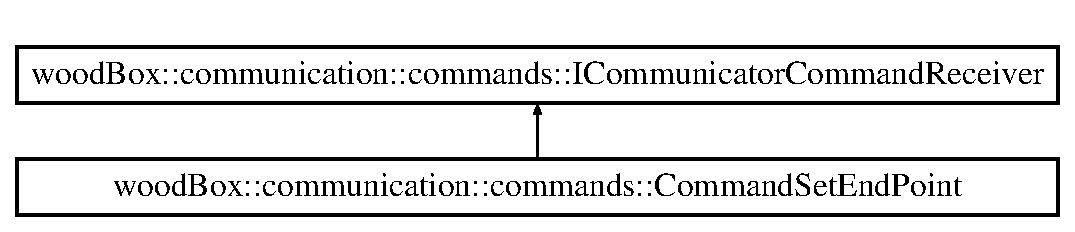
\includegraphics[height=2.000000cm]{classwood_box_1_1communication_1_1commands_1_1_command_set_end_point}
\end{center}
\end{figure}
\subsection*{Public Member Functions}
\begin{DoxyCompactItemize}
\item 
\mbox{\Hypertarget{classwood_box_1_1communication_1_1commands_1_1_command_set_end_point_a52bd7a90eb7e4533d79a09c77940946e}\label{classwood_box_1_1communication_1_1commands_1_1_command_set_end_point_a52bd7a90eb7e4533d79a09c77940946e}} 
{\bfseries Command\+Set\+End\+Point} (\mbox{\hyperlink{classwood_box_1_1communication_1_1wifi_1_1_a_wi_fi_communicator}{wifi\+::\+A\+Wi\+Fi\+Communicator}} \&)
\item 
\mbox{\Hypertarget{classwood_box_1_1communication_1_1commands_1_1_command_set_end_point_abd58a35add8c83a23d80fb8c3a1b6c7d}\label{classwood_box_1_1communication_1_1commands_1_1_command_set_end_point_abd58a35add8c83a23d80fb8c3a1b6c7d}} 
{\bfseries Command\+Set\+End\+Point} (const \mbox{\hyperlink{classwood_box_1_1communication_1_1commands_1_1_command_set_end_point}{Command\+Set\+End\+Point}} \&)=delete
\item 
\mbox{\Hypertarget{classwood_box_1_1communication_1_1commands_1_1_command_set_end_point_a71df3e4cede5be682d49856c8934baf3}\label{classwood_box_1_1communication_1_1commands_1_1_command_set_end_point_a71df3e4cede5be682d49856c8934baf3}} 
\mbox{\hyperlink{classwood_box_1_1communication_1_1commands_1_1_command_set_end_point}{Command\+Set\+End\+Point}} \& {\bfseries operator=} (const \mbox{\hyperlink{classwood_box_1_1communication_1_1commands_1_1_command_set_end_point}{Command\+Set\+End\+Point}} \&)=delete
\item 
\mbox{\Hypertarget{classwood_box_1_1communication_1_1commands_1_1_command_set_end_point_ad11ea4ae0498b70c05b63cef652bc495}\label{classwood_box_1_1communication_1_1commands_1_1_command_set_end_point_ad11ea4ae0498b70c05b63cef652bc495}} 
virtual void {\bfseries parse} (Stream \&)
\item 
\mbox{\Hypertarget{classwood_box_1_1communication_1_1commands_1_1_command_set_end_point_a36b3692b99c49c115b77396462e3cb3e}\label{classwood_box_1_1communication_1_1commands_1_1_command_set_end_point_a36b3692b99c49c115b77396462e3cb3e}} 
virtual void {\bfseries execute} ()
\item 
\mbox{\Hypertarget{classwood_box_1_1communication_1_1commands_1_1_command_set_end_point_a7088dc748dd916406028d1d875d6b708}\label{classwood_box_1_1communication_1_1commands_1_1_command_set_end_point_a7088dc748dd916406028d1d875d6b708}} 
virtual void {\bfseries reply} (Stream \&)
\end{DoxyCompactItemize}


The documentation for this class was generated from the following files\+:\begin{DoxyCompactItemize}
\item 
Command\+Set\+End\+Point.\+hpp\item 
Command\+Set\+End\+Point.\+cpp\end{DoxyCompactItemize}

\hypertarget{classwood_box_1_1communication_1_1commands_1_1_command_set_wi_fi}{}\section{wood\+Box\+:\+:communication\+:\+:commands\+:\+:Command\+Set\+Wi\+Fi Class Reference}
\label{classwood_box_1_1communication_1_1commands_1_1_command_set_wi_fi}\index{wood\+Box\+::communication\+::commands\+::\+Command\+Set\+Wi\+Fi@{wood\+Box\+::communication\+::commands\+::\+Command\+Set\+Wi\+Fi}}
Inheritance diagram for wood\+Box\+:\+:communication\+:\+:commands\+:\+:Command\+Set\+Wi\+Fi\+:\begin{figure}[H]
\begin{center}
\leavevmode
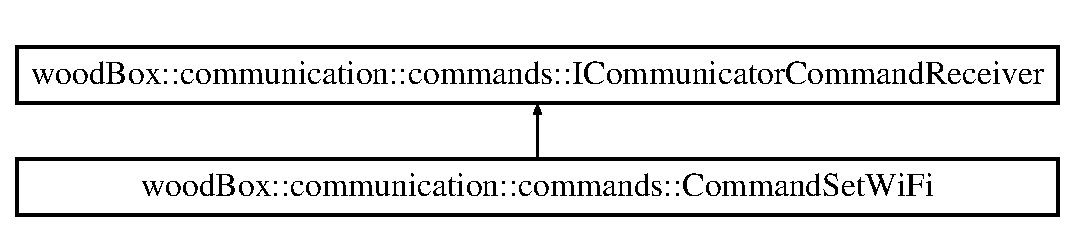
\includegraphics[height=2.000000cm]{classwood_box_1_1communication_1_1commands_1_1_command_set_wi_fi}
\end{center}
\end{figure}
\subsection*{Public Member Functions}
\begin{DoxyCompactItemize}
\item 
\mbox{\Hypertarget{classwood_box_1_1communication_1_1commands_1_1_command_set_wi_fi_ab2a87abf9f2adbfb4274325bc0808d62}\label{classwood_box_1_1communication_1_1commands_1_1_command_set_wi_fi_ab2a87abf9f2adbfb4274325bc0808d62}} 
{\bfseries Command\+Set\+Wi\+Fi} (\mbox{\hyperlink{classwood_box_1_1communication_1_1wifi_1_1_a_wi_fi_communicator}{wifi\+::\+A\+Wi\+Fi\+Communicator}} \&)
\item 
\mbox{\Hypertarget{classwood_box_1_1communication_1_1commands_1_1_command_set_wi_fi_ac2a83301978b8c5caedbfe9550739c6d}\label{classwood_box_1_1communication_1_1commands_1_1_command_set_wi_fi_ac2a83301978b8c5caedbfe9550739c6d}} 
{\bfseries Command\+Set\+Wi\+Fi} (const \mbox{\hyperlink{classwood_box_1_1communication_1_1commands_1_1_command_set_wi_fi}{Command\+Set\+Wi\+Fi}} \&)=delete
\item 
\mbox{\Hypertarget{classwood_box_1_1communication_1_1commands_1_1_command_set_wi_fi_ae75518186c9db39992718bbe09d8e594}\label{classwood_box_1_1communication_1_1commands_1_1_command_set_wi_fi_ae75518186c9db39992718bbe09d8e594}} 
\mbox{\hyperlink{classwood_box_1_1communication_1_1commands_1_1_command_set_wi_fi}{Command\+Set\+Wi\+Fi}} \& {\bfseries operator=} (const \mbox{\hyperlink{classwood_box_1_1communication_1_1commands_1_1_command_set_wi_fi}{Command\+Set\+Wi\+Fi}} \&)=delete
\item 
\mbox{\Hypertarget{classwood_box_1_1communication_1_1commands_1_1_command_set_wi_fi_a1fe9a0798b8502acf76fd787a632b6f1}\label{classwood_box_1_1communication_1_1commands_1_1_command_set_wi_fi_a1fe9a0798b8502acf76fd787a632b6f1}} 
virtual void {\bfseries parse} (Stream \&)
\item 
\mbox{\Hypertarget{classwood_box_1_1communication_1_1commands_1_1_command_set_wi_fi_ad94b980986a752bf0cd5778487313d8f}\label{classwood_box_1_1communication_1_1commands_1_1_command_set_wi_fi_ad94b980986a752bf0cd5778487313d8f}} 
virtual void {\bfseries execute} ()
\item 
\mbox{\Hypertarget{classwood_box_1_1communication_1_1commands_1_1_command_set_wi_fi_a364a4dbaf01a1815e296fc1569665522}\label{classwood_box_1_1communication_1_1commands_1_1_command_set_wi_fi_a364a4dbaf01a1815e296fc1569665522}} 
virtual void {\bfseries reply} (Stream \&)
\end{DoxyCompactItemize}


The documentation for this class was generated from the following files\+:\begin{DoxyCompactItemize}
\item 
Command\+Set\+Wi\+Fi.\+hpp\item 
Command\+Set\+Wi\+Fi.\+cpp\end{DoxyCompactItemize}

\hypertarget{classwood_box_1_1communication_1_1wifi_1_1_e_s_p8266_wi_fi_communicator}{}\section{wood\+Box\+:\+:communication\+:\+:wifi\+:\+:E\+S\+P8266\+Wi\+Fi\+Communicator Class Reference}
\label{classwood_box_1_1communication_1_1wifi_1_1_e_s_p8266_wi_fi_communicator}\index{wood\+Box\+::communication\+::wifi\+::\+E\+S\+P8266\+Wi\+Fi\+Communicator@{wood\+Box\+::communication\+::wifi\+::\+E\+S\+P8266\+Wi\+Fi\+Communicator}}
Inheritance diagram for wood\+Box\+:\+:communication\+:\+:wifi\+:\+:E\+S\+P8266\+Wi\+Fi\+Communicator\+:\begin{figure}[H]
\begin{center}
\leavevmode
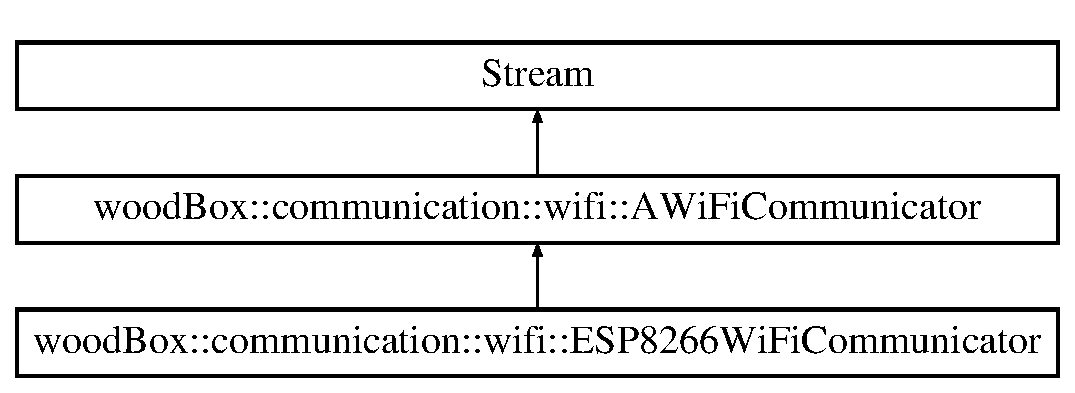
\includegraphics[height=3.000000cm]{classwood_box_1_1communication_1_1wifi_1_1_e_s_p8266_wi_fi_communicator}
\end{center}
\end{figure}
\subsection*{Public Member Functions}
\begin{DoxyCompactItemize}
\item 
\mbox{\Hypertarget{classwood_box_1_1communication_1_1wifi_1_1_e_s_p8266_wi_fi_communicator_a0af11f50c19c8d00112e61e7919294ef}\label{classwood_box_1_1communication_1_1wifi_1_1_e_s_p8266_wi_fi_communicator_a0af11f50c19c8d00112e61e7919294ef}} 
{\bfseries E\+S\+P8266\+Wi\+Fi\+Communicator} (int, int)
\item 
\mbox{\Hypertarget{classwood_box_1_1communication_1_1wifi_1_1_e_s_p8266_wi_fi_communicator_a7e7137815f9b6d8dc18adcef1ccb13cc}\label{classwood_box_1_1communication_1_1wifi_1_1_e_s_p8266_wi_fi_communicator_a7e7137815f9b6d8dc18adcef1ccb13cc}} 
{\bfseries E\+S\+P8266\+Wi\+Fi\+Communicator} (const \mbox{\hyperlink{classwood_box_1_1communication_1_1wifi_1_1_e_s_p8266_wi_fi_communicator}{E\+S\+P8266\+Wi\+Fi\+Communicator}} \&)=delete
\item 
\mbox{\Hypertarget{classwood_box_1_1communication_1_1wifi_1_1_e_s_p8266_wi_fi_communicator_a422e4ef0462beca6e66a5909b41966ef}\label{classwood_box_1_1communication_1_1wifi_1_1_e_s_p8266_wi_fi_communicator_a422e4ef0462beca6e66a5909b41966ef}} 
\mbox{\hyperlink{classwood_box_1_1communication_1_1wifi_1_1_e_s_p8266_wi_fi_communicator}{E\+S\+P8266\+Wi\+Fi\+Communicator}} \& {\bfseries operator=} (const \mbox{\hyperlink{classwood_box_1_1communication_1_1wifi_1_1_e_s_p8266_wi_fi_communicator}{E\+S\+P8266\+Wi\+Fi\+Communicator}} \&)=delete
\item 
\mbox{\Hypertarget{classwood_box_1_1communication_1_1wifi_1_1_e_s_p8266_wi_fi_communicator_aa73f46aaaf5441b79dd4a15be293aeb4}\label{classwood_box_1_1communication_1_1wifi_1_1_e_s_p8266_wi_fi_communicator_aa73f46aaaf5441b79dd4a15be293aeb4}} 
virtual int {\bfseries available} ()
\item 
\mbox{\Hypertarget{classwood_box_1_1communication_1_1wifi_1_1_e_s_p8266_wi_fi_communicator_a3bd1c8f72256e92c6dbdab9272fd3543}\label{classwood_box_1_1communication_1_1wifi_1_1_e_s_p8266_wi_fi_communicator_a3bd1c8f72256e92c6dbdab9272fd3543}} 
virtual int {\bfseries read} ()
\item 
\mbox{\Hypertarget{classwood_box_1_1communication_1_1wifi_1_1_e_s_p8266_wi_fi_communicator_accc6832fa7351cb977b9e3a805dc8107}\label{classwood_box_1_1communication_1_1wifi_1_1_e_s_p8266_wi_fi_communicator_accc6832fa7351cb977b9e3a805dc8107}} 
virtual int {\bfseries peek} ()
\item 
\mbox{\Hypertarget{classwood_box_1_1communication_1_1wifi_1_1_e_s_p8266_wi_fi_communicator_a6bb904e5302da7ec3fefc6e9a896f5f8}\label{classwood_box_1_1communication_1_1wifi_1_1_e_s_p8266_wi_fi_communicator_a6bb904e5302da7ec3fefc6e9a896f5f8}} 
virtual size\+\_\+t {\bfseries write} (uint8\+\_\+t)
\item 
\mbox{\Hypertarget{classwood_box_1_1communication_1_1wifi_1_1_e_s_p8266_wi_fi_communicator_a523aec958ef48fa917621a560d964f40}\label{classwood_box_1_1communication_1_1wifi_1_1_e_s_p8266_wi_fi_communicator_a523aec958ef48fa917621a560d964f40}} 
virtual void {\bfseries flush} ()
\item 
\mbox{\Hypertarget{classwood_box_1_1communication_1_1wifi_1_1_e_s_p8266_wi_fi_communicator_a8bf593dd2b78572988c240b57cc9c5c8}\label{classwood_box_1_1communication_1_1wifi_1_1_e_s_p8266_wi_fi_communicator_a8bf593dd2b78572988c240b57cc9c5c8}} 
void {\bfseries open} ()
\item 
\mbox{\Hypertarget{classwood_box_1_1communication_1_1wifi_1_1_e_s_p8266_wi_fi_communicator_ae8188b06891b3fd0e21312b3e69910d4}\label{classwood_box_1_1communication_1_1wifi_1_1_e_s_p8266_wi_fi_communicator_ae8188b06891b3fd0e21312b3e69910d4}} 
void {\bfseries close} ()
\item 
\mbox{\Hypertarget{classwood_box_1_1communication_1_1wifi_1_1_e_s_p8266_wi_fi_communicator_ab3e1f12a851dc3ed6eb487c39178cb6f}\label{classwood_box_1_1communication_1_1wifi_1_1_e_s_p8266_wi_fi_communicator_ab3e1f12a851dc3ed6eb487c39178cb6f}} 
virtual int {\bfseries connect} ()
\item 
\mbox{\Hypertarget{classwood_box_1_1communication_1_1wifi_1_1_e_s_p8266_wi_fi_communicator_af30a81a7f279c11241b3df0878289af0}\label{classwood_box_1_1communication_1_1wifi_1_1_e_s_p8266_wi_fi_communicator_af30a81a7f279c11241b3df0878289af0}} 
virtual int {\bfseries disconnect} ()
\item 
\mbox{\Hypertarget{classwood_box_1_1communication_1_1wifi_1_1_e_s_p8266_wi_fi_communicator_a0875cf7209c48069d22270eaeb2cac0f}\label{classwood_box_1_1communication_1_1wifi_1_1_e_s_p8266_wi_fi_communicator_a0875cf7209c48069d22270eaeb2cac0f}} 
virtual int {\bfseries connect\+To\+Host} ()
\item 
\mbox{\Hypertarget{classwood_box_1_1communication_1_1wifi_1_1_e_s_p8266_wi_fi_communicator_a5a407734df1ae47ac32575fa6346cfd4}\label{classwood_box_1_1communication_1_1wifi_1_1_e_s_p8266_wi_fi_communicator_a5a407734df1ae47ac32575fa6346cfd4}} 
virtual int {\bfseries disconnect\+From\+Host} ()
\item 
\mbox{\Hypertarget{classwood_box_1_1communication_1_1wifi_1_1_e_s_p8266_wi_fi_communicator_a66b7f8adaae85dbf94062b1cd472d98a}\label{classwood_box_1_1communication_1_1wifi_1_1_e_s_p8266_wi_fi_communicator_a66b7f8adaae85dbf94062b1cd472d98a}} 
virtual bool {\bfseries is\+Connected} ()
\end{DoxyCompactItemize}
\subsection*{Additional Inherited Members}


The documentation for this class was generated from the following files\+:\begin{DoxyCompactItemize}
\item 
E\+S\+P8266\+Wi\+Fi\+Communicator.\+hpp\item 
E\+S\+P8266\+Wi\+Fi\+Communicator.\+cpp\end{DoxyCompactItemize}

\hypertarget{classwood_box_1_1communication_1_1_i_communicator}{}\section{wood\+Box\+:\+:communication\+:\+:I\+Communicator Class Reference}
\label{classwood_box_1_1communication_1_1_i_communicator}\index{wood\+Box\+::communication\+::\+I\+Communicator@{wood\+Box\+::communication\+::\+I\+Communicator}}
Inheritance diagram for wood\+Box\+:\+:communication\+:\+:I\+Communicator\+:\begin{figure}[H]
\begin{center}
\leavevmode
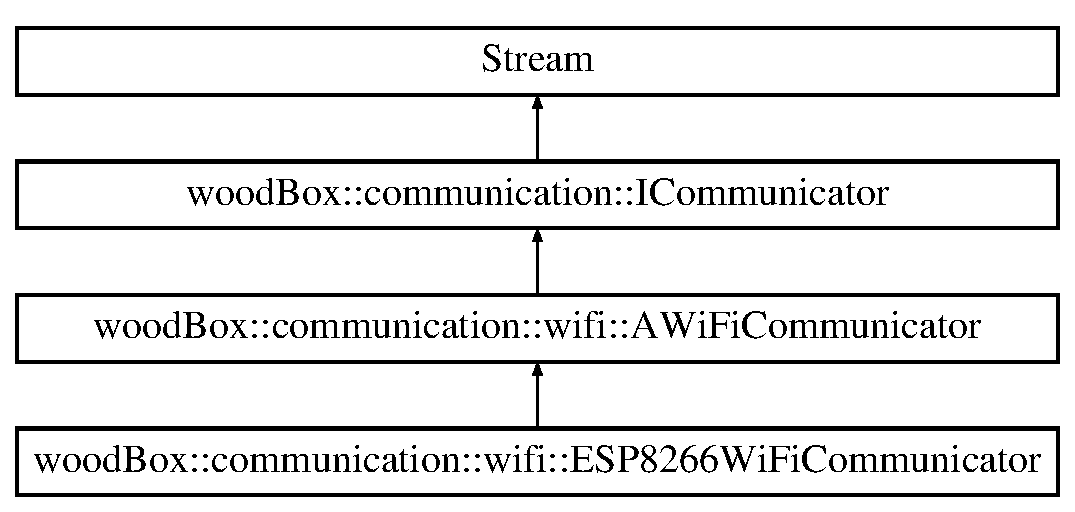
\includegraphics[height=3.000000cm]{classwood_box_1_1communication_1_1_i_communicator}
\end{center}
\end{figure}
\subsection*{Public Member Functions}
\begin{DoxyCompactItemize}
\item 
\mbox{\Hypertarget{classwood_box_1_1communication_1_1_i_communicator_abc731c594645f869db95a557e387958d}\label{classwood_box_1_1communication_1_1_i_communicator_abc731c594645f869db95a557e387958d}} 
virtual void {\bfseries open} ()=0
\item 
\mbox{\Hypertarget{classwood_box_1_1communication_1_1_i_communicator_afca0e27bcc0c65273c7e020dc30145fb}\label{classwood_box_1_1communication_1_1_i_communicator_afca0e27bcc0c65273c7e020dc30145fb}} 
virtual void {\bfseries close} ()=0
\end{DoxyCompactItemize}


The documentation for this class was generated from the following file\+:\begin{DoxyCompactItemize}
\item 
I\+Communicator.\+hpp\end{DoxyCompactItemize}

\hypertarget{classwood_box_1_1communication_1_1commands_1_1_i_communicator_command_receiver}{}\section{wood\+Box\+:\+:communication\+:\+:commands\+:\+:I\+Communicator\+Command\+Receiver Class Reference}
\label{classwood_box_1_1communication_1_1commands_1_1_i_communicator_command_receiver}\index{wood\+Box\+::communication\+::commands\+::\+I\+Communicator\+Command\+Receiver@{wood\+Box\+::communication\+::commands\+::\+I\+Communicator\+Command\+Receiver}}
Inheritance diagram for wood\+Box\+:\+:communication\+:\+:commands\+:\+:I\+Communicator\+Command\+Receiver\+:\begin{figure}[H]
\begin{center}
\leavevmode
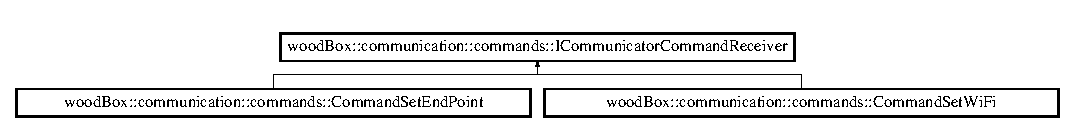
\includegraphics[height=2.000000cm]{classwood_box_1_1communication_1_1commands_1_1_i_communicator_command_receiver}
\end{center}
\end{figure}
\subsection*{Public Member Functions}
\begin{DoxyCompactItemize}
\item 
\mbox{\Hypertarget{classwood_box_1_1communication_1_1commands_1_1_i_communicator_command_receiver_a726577de1e09ad34edc9670ee8f9836f}\label{classwood_box_1_1communication_1_1commands_1_1_i_communicator_command_receiver_a726577de1e09ad34edc9670ee8f9836f}} 
virtual void {\bfseries parse} (\mbox{\hyperlink{classwood_box_1_1communication_1_1_i_communicator}{I\+Communicator}} \&)=0
\item 
\mbox{\Hypertarget{classwood_box_1_1communication_1_1commands_1_1_i_communicator_command_receiver_a071207a1c875f6a34e6954cc8195b634}\label{classwood_box_1_1communication_1_1commands_1_1_i_communicator_command_receiver_a071207a1c875f6a34e6954cc8195b634}} 
virtual void {\bfseries execute} ()=0
\item 
\mbox{\Hypertarget{classwood_box_1_1communication_1_1commands_1_1_i_communicator_command_receiver_a268eff00d15b5c1bd7f597f8ce93b474}\label{classwood_box_1_1communication_1_1commands_1_1_i_communicator_command_receiver_a268eff00d15b5c1bd7f597f8ce93b474}} 
virtual void {\bfseries reply} (\mbox{\hyperlink{classwood_box_1_1communication_1_1_i_communicator}{I\+Communicator}} \&)=0
\end{DoxyCompactItemize}


The documentation for this class was generated from the following file\+:\begin{DoxyCompactItemize}
\item 
I\+Communicator\+Event\+Receiver.\+hpp\end{DoxyCompactItemize}

\hypertarget{classwood_box_1_1display_1_1_i_display}{}\section{wood\+Box\+:\+:display\+:\+:I\+Display Class Reference}
\label{classwood_box_1_1display_1_1_i_display}\index{wood\+Box\+::display\+::\+I\+Display@{wood\+Box\+::display\+::\+I\+Display}}
Inheritance diagram for wood\+Box\+:\+:display\+:\+:I\+Display\+:\begin{figure}[H]
\begin{center}
\leavevmode
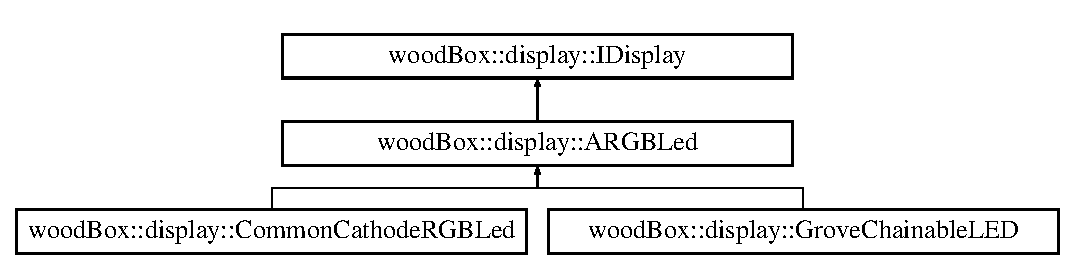
\includegraphics[height=2.000000cm]{classwood_box_1_1display_1_1_i_display}
\end{center}
\end{figure}
\subsection*{Public Member Functions}
\begin{DoxyCompactItemize}
\item 
\mbox{\Hypertarget{classwood_box_1_1display_1_1_i_display_a7030f0768c1ef15ce936a259406168dc}\label{classwood_box_1_1display_1_1_i_display_a7030f0768c1ef15ce936a259406168dc}} 
virtual void {\bfseries clear} ()=0
\item 
\mbox{\Hypertarget{classwood_box_1_1display_1_1_i_display_ad8c0811b8b807ce119a06c7806004de7}\label{classwood_box_1_1display_1_1_i_display_ad8c0811b8b807ce119a06c7806004de7}} 
virtual void {\bfseries update} ()=0
\end{DoxyCompactItemize}


The documentation for this class was generated from the following file\+:\begin{DoxyCompactItemize}
\item 
I\+Display.\+hpp\end{DoxyCompactItemize}

\hypertarget{classwood_box_1_1module_1_1_i_module}{}\section{wood\+Box\+:\+:module\+:\+:I\+Module Class Reference}
\label{classwood_box_1_1module_1_1_i_module}\index{wood\+Box\+::module\+::\+I\+Module@{wood\+Box\+::module\+::\+I\+Module}}
Inheritance diagram for wood\+Box\+:\+:module\+:\+:I\+Module\+:\begin{figure}[H]
\begin{center}
\leavevmode
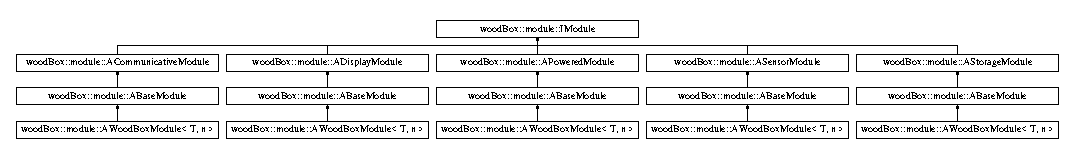
\includegraphics[height=1.635036cm]{classwood_box_1_1module_1_1_i_module}
\end{center}
\end{figure}
\subsection*{Public Member Functions}
\begin{DoxyCompactItemize}
\item 
\mbox{\Hypertarget{classwood_box_1_1module_1_1_i_module_a01228121e79242942fc365060b3a9ab9}\label{classwood_box_1_1module_1_1_i_module_a01228121e79242942fc365060b3a9ab9}} 
virtual void {\bfseries run} ()=0
\item 
\mbox{\Hypertarget{classwood_box_1_1module_1_1_i_module_a32bdfa5bcdd901598c617587869cbec3}\label{classwood_box_1_1module_1_1_i_module_a32bdfa5bcdd901598c617587869cbec3}} 
virtual void {\bfseries stop} ()=0
\end{DoxyCompactItemize}


The documentation for this class was generated from the following file\+:\begin{DoxyCompactItemize}
\item 
I\+Module.\+hpp\end{DoxyCompactItemize}

\hypertarget{classwood_box_1_1power_1_1_i_power}{}\section{wood\+Box\+:\+:power\+:\+:I\+Power Class Reference}
\label{classwood_box_1_1power_1_1_i_power}\index{wood\+Box\+::power\+::\+I\+Power@{wood\+Box\+::power\+::\+I\+Power}}
\subsection*{Public Member Functions}
\begin{DoxyCompactItemize}
\item 
\mbox{\Hypertarget{classwood_box_1_1power_1_1_i_power_a4645f7d9dbbaee583ba2446ef35a8635}\label{classwood_box_1_1power_1_1_i_power_a4645f7d9dbbaee583ba2446ef35a8635}} 
virtual bool {\bfseries is\+Working} ()=0
\item 
\mbox{\Hypertarget{classwood_box_1_1power_1_1_i_power_a67086e56aca8cb46033a441b3f4e11aa}\label{classwood_box_1_1power_1_1_i_power_a67086e56aca8cb46033a441b3f4e11aa}} 
virtual uint32\+\_\+t {\bfseries get\+Voltage} ()=0
\item 
\mbox{\Hypertarget{classwood_box_1_1power_1_1_i_power_a9b3e0363c22d3064bd7ccc8663f1a033}\label{classwood_box_1_1power_1_1_i_power_a9b3e0363c22d3064bd7ccc8663f1a033}} 
virtual uint32\+\_\+t {\bfseries get\+Current} ()=0
\end{DoxyCompactItemize}


The documentation for this class was generated from the following file\+:\begin{DoxyCompactItemize}
\item 
I\+Power.\+hpp\end{DoxyCompactItemize}

\hypertarget{classwood_box_1_1display_1_1_i_r_g_b_led}{}\section{wood\+Box\+:\+:display\+:\+:I\+R\+G\+B\+Led Class Reference}
\label{classwood_box_1_1display_1_1_i_r_g_b_led}\index{wood\+Box\+::display\+::\+I\+R\+G\+B\+Led@{wood\+Box\+::display\+::\+I\+R\+G\+B\+Led}}
Inheritance diagram for wood\+Box\+:\+:display\+:\+:I\+R\+G\+B\+Led\+:\begin{figure}[H]
\begin{center}
\leavevmode
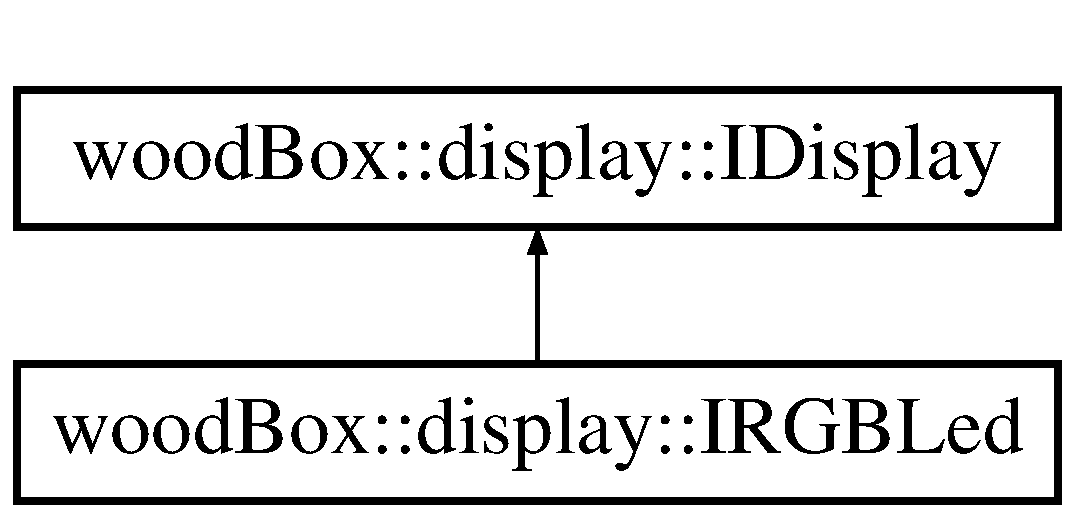
\includegraphics[height=2.000000cm]{classwood_box_1_1display_1_1_i_r_g_b_led}
\end{center}
\end{figure}
\subsection*{Classes}
\begin{DoxyCompactItemize}
\item 
struct \mbox{\hyperlink{structwood_box_1_1display_1_1_i_r_g_b_led_1_1_color}{Color}}
\end{DoxyCompactItemize}
\subsection*{Public Member Functions}
\begin{DoxyCompactItemize}
\item 
\mbox{\Hypertarget{classwood_box_1_1display_1_1_i_r_g_b_led_a023df51cd4d84ac74f3c489428b5bc3c}\label{classwood_box_1_1display_1_1_i_r_g_b_led_a023df51cd4d84ac74f3c489428b5bc3c}} 
virtual void {\bfseries clear} ()=0
\item 
\mbox{\Hypertarget{classwood_box_1_1display_1_1_i_r_g_b_led_a41a5a8a358a7e7ae337741f1f3ca7186}\label{classwood_box_1_1display_1_1_i_r_g_b_led_a41a5a8a358a7e7ae337741f1f3ca7186}} 
virtual void {\bfseries update} ()=0
\item 
\mbox{\Hypertarget{classwood_box_1_1display_1_1_i_r_g_b_led_a770327a3dd8526bef31fe763cfb76462}\label{classwood_box_1_1display_1_1_i_r_g_b_led_a770327a3dd8526bef31fe763cfb76462}} 
virtual const \mbox{\hyperlink{structwood_box_1_1display_1_1_i_r_g_b_led_1_1_color}{Color}} \& {\bfseries get\+Color} () const =0
\item 
\mbox{\Hypertarget{classwood_box_1_1display_1_1_i_r_g_b_led_a3465053e8bf6ed7cfd1990f15d856ed7}\label{classwood_box_1_1display_1_1_i_r_g_b_led_a3465053e8bf6ed7cfd1990f15d856ed7}} 
virtual void {\bfseries set\+Color} (const \mbox{\hyperlink{structwood_box_1_1display_1_1_i_r_g_b_led_1_1_color}{Color}} \&)=0
\end{DoxyCompactItemize}


The documentation for this class was generated from the following file\+:\begin{DoxyCompactItemize}
\item 
I\+R\+G\+B\+Led.\+hpp\end{DoxyCompactItemize}

\hypertarget{classwood_box_1_1sensor_1_1_i_sensor}{}\section{wood\+Box\+:\+:sensor\+:\+:I\+Sensor Class Reference}
\label{classwood_box_1_1sensor_1_1_i_sensor}\index{wood\+Box\+::sensor\+::\+I\+Sensor@{wood\+Box\+::sensor\+::\+I\+Sensor}}
Inheritance diagram for wood\+Box\+:\+:sensor\+:\+:I\+Sensor\+:\begin{figure}[H]
\begin{center}
\leavevmode
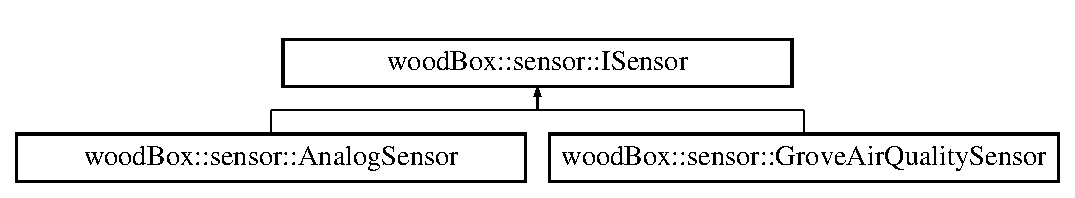
\includegraphics[height=2.000000cm]{classwood_box_1_1sensor_1_1_i_sensor}
\end{center}
\end{figure}
\subsection*{Public Member Functions}
\begin{DoxyCompactItemize}
\item 
\mbox{\Hypertarget{classwood_box_1_1sensor_1_1_i_sensor_ac772909aea9d8556cdda19841d3bbc40}\label{classwood_box_1_1sensor_1_1_i_sensor_ac772909aea9d8556cdda19841d3bbc40}} 
virtual void {\bfseries init} ()=0
\item 
\mbox{\Hypertarget{classwood_box_1_1sensor_1_1_i_sensor_a801f29792a0cd49bef0c54b346c570ad}\label{classwood_box_1_1sensor_1_1_i_sensor_a801f29792a0cd49bef0c54b346c570ad}} 
virtual void {\bfseries stop} ()=0
\item 
\mbox{\Hypertarget{classwood_box_1_1sensor_1_1_i_sensor_a9de8041b991b76cc2f6fcc3b6a1bf363}\label{classwood_box_1_1sensor_1_1_i_sensor_a9de8041b991b76cc2f6fcc3b6a1bf363}} 
virtual uint8\+\_\+t $\ast$ {\bfseries get\+Sample} ()=0
\end{DoxyCompactItemize}


The documentation for this class was generated from the following file\+:\begin{DoxyCompactItemize}
\item 
I\+Sensor.\+hpp\end{DoxyCompactItemize}

\hypertarget{classwood_box_1_1storage_1_1_i_storage}{}\section{wood\+Box\+:\+:storage\+:\+:I\+Storage Class Reference}
\label{classwood_box_1_1storage_1_1_i_storage}\index{wood\+Box\+::storage\+::\+I\+Storage@{wood\+Box\+::storage\+::\+I\+Storage}}


{\ttfamily \#include $<$I\+Storage.\+hpp$>$}

\subsection*{Public Member Functions}
\begin{DoxyCompactItemize}
\item 
virtual void \mbox{\hyperlink{classwood_box_1_1storage_1_1_i_storage_a01bab924be0844e3866b27279caa506d}{read}} (size\+\_\+t, void $\ast$, size\+\_\+t)=0
\item 
virtual void \mbox{\hyperlink{classwood_box_1_1storage_1_1_i_storage_a5eb82c922e8a3147ddab510706be8e24}{write}} (size\+\_\+t, const void $\ast$, size\+\_\+t)=0
\end{DoxyCompactItemize}


\subsection{Detailed Description}
Interface used to be able to store and read raw data from any source, by transferring memory buffers 

\subsection{Member Function Documentation}
\mbox{\Hypertarget{classwood_box_1_1storage_1_1_i_storage_a01bab924be0844e3866b27279caa506d}\label{classwood_box_1_1storage_1_1_i_storage_a01bab924be0844e3866b27279caa506d}} 
\index{wood\+Box\+::storage\+::\+I\+Storage@{wood\+Box\+::storage\+::\+I\+Storage}!read@{read}}
\index{read@{read}!wood\+Box\+::storage\+::\+I\+Storage@{wood\+Box\+::storage\+::\+I\+Storage}}
\subsubsection{\texorpdfstring{read()}{read()}}
{\footnotesize\ttfamily virtual void wood\+Box\+::storage\+::\+I\+Storage\+::read (\begin{DoxyParamCaption}\item[{size\+\_\+t}]{,  }\item[{void $\ast$}]{,  }\item[{size\+\_\+t}]{ }\end{DoxyParamCaption})\hspace{0.3cm}{\ttfamily [pure virtual]}}

Copy n bytes (3rd parameter) in dest (2nd parameter) from offset x (1st parameter) \mbox{\Hypertarget{classwood_box_1_1storage_1_1_i_storage_a5eb82c922e8a3147ddab510706be8e24}\label{classwood_box_1_1storage_1_1_i_storage_a5eb82c922e8a3147ddab510706be8e24}} 
\index{wood\+Box\+::storage\+::\+I\+Storage@{wood\+Box\+::storage\+::\+I\+Storage}!write@{write}}
\index{write@{write}!wood\+Box\+::storage\+::\+I\+Storage@{wood\+Box\+::storage\+::\+I\+Storage}}
\subsubsection{\texorpdfstring{write()}{write()}}
{\footnotesize\ttfamily virtual void wood\+Box\+::storage\+::\+I\+Storage\+::write (\begin{DoxyParamCaption}\item[{size\+\_\+t}]{,  }\item[{const void $\ast$}]{,  }\item[{size\+\_\+t}]{ }\end{DoxyParamCaption})\hspace{0.3cm}{\ttfamily [pure virtual]}}

Write n bytes (3rd parameter) in offset x (1st parameter) from src (2nd parameter) 

The documentation for this class was generated from the following file\+:\begin{DoxyCompactItemize}
\item 
I\+Storage.\+hpp\end{DoxyCompactItemize}

\hypertarget{classwood_box_1_1utility_1_1_queue}{}\section{wood\+Box\+:\+:utility\+:\+:Queue$<$ T $>$ Class Template Reference}
\label{classwood_box_1_1utility_1_1_queue}\index{wood\+Box\+::utility\+::\+Queue$<$ T $>$@{wood\+Box\+::utility\+::\+Queue$<$ T $>$}}
Inheritance diagram for wood\+Box\+:\+:utility\+:\+:Queue$<$ T $>$\+:\begin{figure}[H]
\begin{center}
\leavevmode
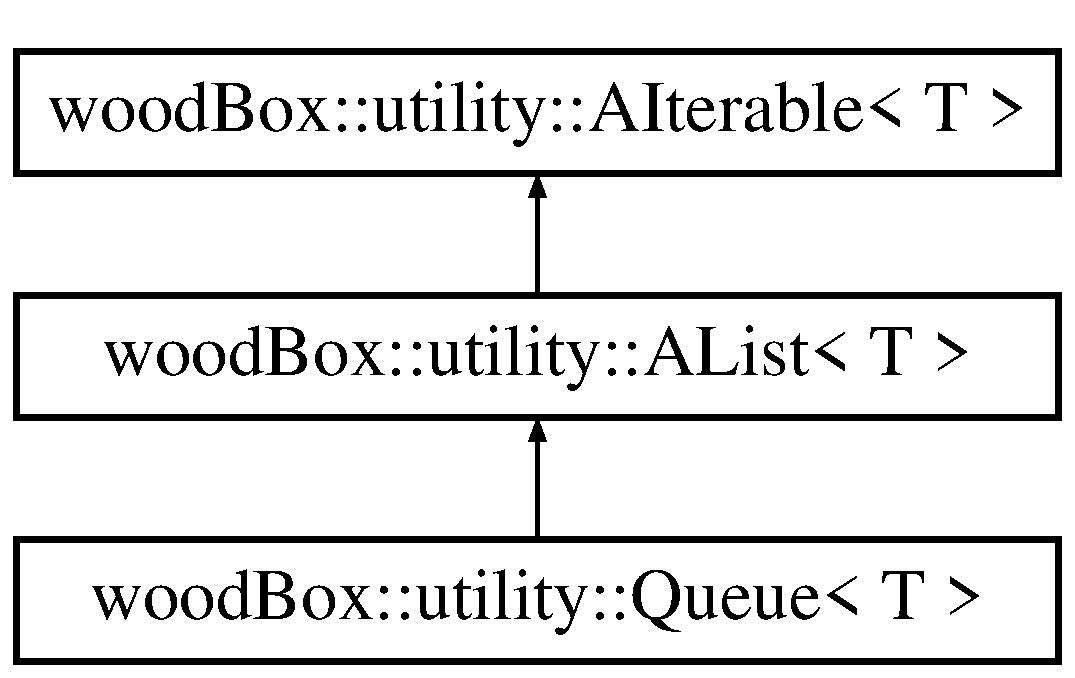
\includegraphics[height=3.000000cm]{classwood_box_1_1utility_1_1_queue}
\end{center}
\end{figure}
\subsection*{Public Member Functions}
\begin{DoxyCompactItemize}
\item 
\mbox{\Hypertarget{classwood_box_1_1utility_1_1_queue_a3fd68bd9b7d12606445926b4e26e763c}\label{classwood_box_1_1utility_1_1_queue_a3fd68bd9b7d12606445926b4e26e763c}} 
{\bfseries Queue} (T \&data)
\item 
\mbox{\Hypertarget{classwood_box_1_1utility_1_1_queue_a811d00da7a7cefd7e3551a1381396a96}\label{classwood_box_1_1utility_1_1_queue_a811d00da7a7cefd7e3551a1381396a96}} 
{\bfseries Queue} (const \mbox{\hyperlink{classwood_box_1_1utility_1_1_queue}{Queue}} \&)=delete
\item 
\mbox{\Hypertarget{classwood_box_1_1utility_1_1_queue_a2c9fea4bcd5ee866d5d81b80a4ff6c6d}\label{classwood_box_1_1utility_1_1_queue_a2c9fea4bcd5ee866d5d81b80a4ff6c6d}} 
\mbox{\hyperlink{classwood_box_1_1utility_1_1_queue}{Queue}} \& {\bfseries operator=} (const \mbox{\hyperlink{classwood_box_1_1utility_1_1_queue}{Queue}} \&)=delete
\item 
\mbox{\Hypertarget{classwood_box_1_1utility_1_1_queue_a027d2b2c9fe678f913ddaf462b37669c}\label{classwood_box_1_1utility_1_1_queue_a027d2b2c9fe678f913ddaf462b37669c}} 
\mbox{\hyperlink{classwood_box_1_1utility_1_1_queue}{Queue}} \& {\bfseries append} (T \&data)
\end{DoxyCompactItemize}
\subsection*{Additional Inherited Members}


The documentation for this class was generated from the following file\+:\begin{DoxyCompactItemize}
\item 
Queue.\+hpp\end{DoxyCompactItemize}

\hypertarget{structs__host}{}\section{s\+\_\+host Struct Reference}
\label{structs__host}\index{s\+\_\+host@{s\+\_\+host}}
\subsection*{Public Attributes}
\begin{DoxyCompactItemize}
\item 
\mbox{\Hypertarget{structs__host_ab70be45f69118b58bfef83d602dea7f0}\label{structs__host_ab70be45f69118b58bfef83d602dea7f0}} 
\begin{tabbing}
xx\=xx\=xx\=xx\=xx\=xx\=xx\=xx\=xx\=\kill
union \{\\
\>ipv6\_address {\bfseries ipv6}\\
\>ipv4\_address {\bfseries ipv4}\\
\}; \\

\end{tabbing}\item 
\mbox{\Hypertarget{structs__host_ae9b1efdcd63ad03473d939bd2ae5ebdf}\label{structs__host_ae9b1efdcd63ad03473d939bd2ae5ebdf}} 
port {\bfseries hport}
\end{DoxyCompactItemize}


The documentation for this struct was generated from the following file\+:\begin{DoxyCompactItemize}
\item 
network\+\_\+ip\+\_\+types.\+hpp\end{DoxyCompactItemize}

\hypertarget{structs__wifi__access__point}{}\section{s\+\_\+wifi\+\_\+access\+\_\+point Struct Reference}
\label{structs__wifi__access__point}\index{s\+\_\+wifi\+\_\+access\+\_\+point@{s\+\_\+wifi\+\_\+access\+\_\+point}}
\subsection*{Public Attributes}
\begin{DoxyCompactItemize}
\item 
\mbox{\Hypertarget{structs__wifi__access__point_a838f0f789f6b491264b7a80368f2bf79}\label{structs__wifi__access__point_a838f0f789f6b491264b7a80368f2bf79}} 
wifi\+\_\+ssid {\bfseries ssid}
\item 
\mbox{\Hypertarget{structs__wifi__access__point_addbd8538051734cf788f9309afa5fb41}\label{structs__wifi__access__point_addbd8538051734cf788f9309afa5fb41}} 
wifi\+\_\+password {\bfseries password}
\item 
\mbox{\Hypertarget{structs__wifi__access__point_ae1b6af887030b3fd096c51852667b1a2}\label{structs__wifi__access__point_ae1b6af887030b3fd096c51852667b1a2}} 
wifi\+\_\+channel {\bfseries channel}
\item 
\mbox{\Hypertarget{structs__wifi__access__point_a4d2b86f50607942d75dfa43c910f0021}\label{structs__wifi__access__point_a4d2b86f50607942d75dfa43c910f0021}} 
wifi\+\_\+norm {\bfseries norm}
\item 
\mbox{\Hypertarget{structs__wifi__access__point_abe261f7eaf54825ff511118a034c8a12}\label{structs__wifi__access__point_abe261f7eaf54825ff511118a034c8a12}} 
wifi\+\_\+frequency\+\_\+band {\bfseries band}
\end{DoxyCompactItemize}


The documentation for this struct was generated from the following file\+:\begin{DoxyCompactItemize}
\item 
wifi\+\_\+types.\+hpp\end{DoxyCompactItemize}

\hypertarget{structs__wifi__client}{}\section{s\+\_\+wifi\+\_\+client Struct Reference}
\label{structs__wifi__client}\index{s\+\_\+wifi\+\_\+client@{s\+\_\+wifi\+\_\+client}}
\subsection*{Public Attributes}
\begin{DoxyCompactItemize}
\item 
\mbox{\Hypertarget{structs__wifi__client_a85dfa454d10da3f08159844ffe0d2327}\label{structs__wifi__client_a85dfa454d10da3f08159844ffe0d2327}} 
mac\+\_\+address {\bfseries mac}
\item 
\mbox{\Hypertarget{structs__wifi__client_abd300c588df84be75b3910e7669b1ea5}\label{structs__wifi__client_abd300c588df84be75b3910e7669b1ea5}} 
ipv4\+\_\+address {\bfseries ipv4}
\item 
\mbox{\Hypertarget{structs__wifi__client_affe4669096f72824606316d9d102eb5c}\label{structs__wifi__client_affe4669096f72824606316d9d102eb5c}} 
ipv6\+\_\+address {\bfseries ipv6}
\end{DoxyCompactItemize}


The documentation for this struct was generated from the following file\+:\begin{DoxyCompactItemize}
\item 
wifi\+\_\+types.\+hpp\end{DoxyCompactItemize}

\hypertarget{classwood_box_1_1utility_1_1_stream_buffer}{}\section{wood\+Box\+:\+:utility\+:\+:Stream\+Buffer$<$ size $>$ Class Template Reference}
\label{classwood_box_1_1utility_1_1_stream_buffer}\index{wood\+Box\+::utility\+::\+Stream\+Buffer$<$ size $>$@{wood\+Box\+::utility\+::\+Stream\+Buffer$<$ size $>$}}
Inheritance diagram for wood\+Box\+:\+:utility\+:\+:Stream\+Buffer$<$ size $>$\+:\begin{figure}[H]
\begin{center}
\leavevmode
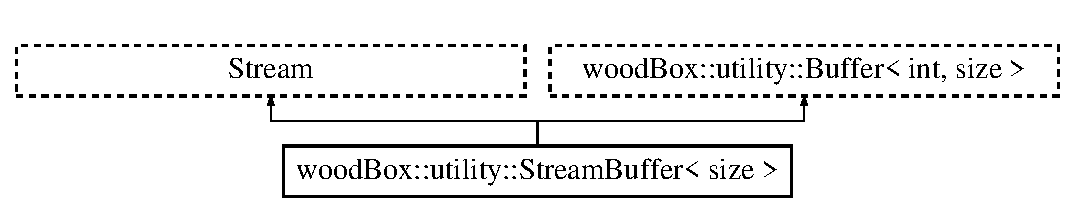
\includegraphics[height=2.000000cm]{classwood_box_1_1utility_1_1_stream_buffer}
\end{center}
\end{figure}
\subsection*{Additional Inherited Members}


The documentation for this class was generated from the following file\+:\begin{DoxyCompactItemize}
\item 
Buffer.\+hpp\end{DoxyCompactItemize}

%--- End generated contents ---

% Index
\backmatter
\newpage
\phantomsection
\clearemptydoublepage
\addcontentsline{toc}{chapter}{Index}
\printindex

\end{document}
